\documentclass[aspectratio=169]{beamer}


\mode<presentation>
{
	\usetheme{default}
	\usecolortheme{beaver}
	\usefonttheme{default}
	\setbeamertemplate{navigation symbols}{}
	\setbeamertemplate{caption}[numbered]
}

%enumerate continuing numbering
\setbeamercovered{highly dynamic}

\newcounter{saveenumi}
\newcommand{\seti}{\setcounter{saveenumi}{\value{enumi}}}
\newcommand{\conti}{\setcounter{enumi}{\value{saveenumi}}}
%

\usepackage[portuguese]{babel}
\usepackage[utf8x]{inputenc}
\usepackage[T1]{fontenc}
\usepackage{natbib}
\usepackage{hyperref}
\usepackage{enumerate}
\usepackage{subfig}
%\usepackage{biblatex}
\usepackage{booktabs} % To thicken table lines

%numbering
\addtobeamertemplate{navigation symbols}{}{%
	\usebeamerfont{footline}%
	\usebeamercolor[fg]{footline}%
	\hspace{1em}%
	\insertframenumber/\inserttotalframenumber
}

\title[Proposta de tese para o exame de qualificação]{Aprimoramentos em modelagem geológica implícita com funções distância assinaladas}
%\subtitle{Proposta de tese para o exame de qualificação}
\author{Me. Roberto Mentzingen Rolo \\ \small{Orientador: Prof. Dr. João Felipe Coimbra Leite Costa, PhD}}
\institute{Universidade Federal do Rio Grande do Sul \\ Escola de Engenharia \\ Programa de Pós-Graduação em Engenharia de Minas, Metalúrgica e de Materiais}
\date{17 de junho de 2019}

\begin{document}
	
%\section{Apresentação}
	
\begin{frame}
	\titlepage
\end{frame}

%sumário
\begin{frame}[allowframebreaks]{sumário}
\tableofcontents
\end{frame}

\section{Introdução}

\begin{frame}{Introdução}

Construir modelos numéricos de longo, médio e curto prazo para avaliação de recursos/reservas e planejamento de mina exige quatro grandes atividades:

\begin{enumerate}
\item Coleta e gerenciamento de dados;
\item Interpretação e modelagem geológica;
\item Atribuição de teores;
\item Avaliação e gerenciamento da incerteza geológica e de teores.
\end{enumerate}

\end{frame}

\subsection{Interpretação e modelagem geológica}

\begin{frame}{Interpretação e modelagem geológica}

\begin{enumerate}
	\item Identificar diferentes domínios;
	\item Definir os limites de cada função aleatória estacionária.
\end{enumerate}

\begin{figure}[H]
	\begin{center}
		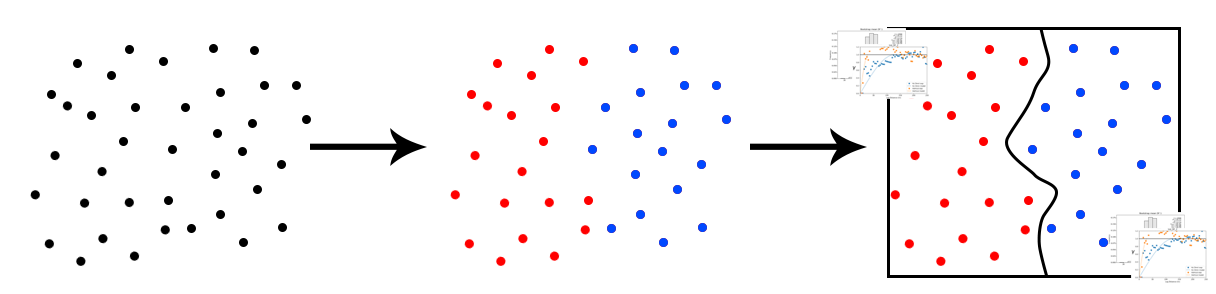
\includegraphics[width=\textwidth]{apresentacao/passo_2}
		\caption{Interpretação e modelagem geológica.}
	\end{center}
\end{figure}

\end{frame}

\subsection{Método tradicional}

\begin{frame}{Metodologia tradicional}

A abordagem tradicional para a criação de modelos geológicos tridimensionais é através da triangulação de polilinhas.

\begin{figure}[H]
	\begin{center}
		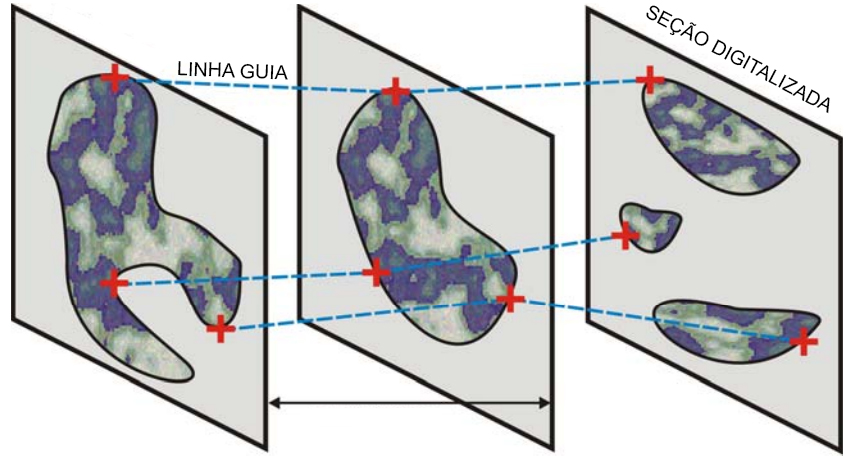
\includegraphics[width=0.6\textwidth]{capitulo_1/explicitmodeling}
		\caption{Esquema do método tradicional.}
	\end{center}
\end{figure}

\end{frame}

\begin{frame}{Desvantagens do método tradicional}
	\begin{itemize}
		\item Tedioso e demorado;
		\item Exige um profissional especializado e experiente;
		\item Geometria dos corpos precisa ser simplificada;
		\item Subjetivo;
		\item Não replicável;
		\item Inflexível;
		\item Não avalia a incerteza.
	\end{itemize}
\end{frame}

\subsection{Incerteza do modelo geológico}

\begin{frame}{Incerteza do modelo geológico}

Em muitos casos, a incerteza do modelo geológico pode ser uma fonte de incerteza crucial e deve ser avaliada.

\begin{figure}[H]
	\begin{center}
		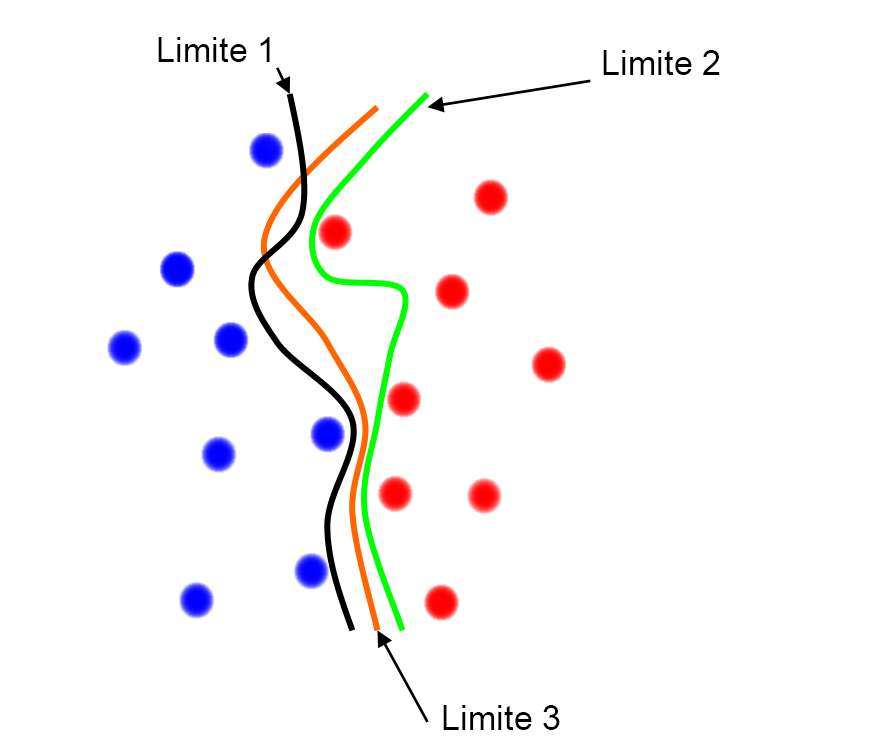
\includegraphics[width=0.4\textwidth]{capitulo_1/incerteza_limites}
		\caption{Incerteza do modelo geológico.}
	\end{center}
\end{figure}
\end{frame}

\subsection{Métodos matemáticos}

\begin{frame}{Métodos matemáticos}

	\begin{columns}[t]
		\begin{column}{0.5\textwidth}
			\begin{center}
				\textit{Métodos determinísticos}
			\end{center}
			\begin{itemize}
				\item Vizinho mais próximo;
				\item Krigagem dos indicadores.
			\end{itemize}
		\end{column}
		\begin{column}{0.5\textwidth}
			\begin{center}
				\textit{Métodos estocásticos}
			\end{center}
			\begin{itemize}
				\item Simulação sequencial dos indicadores;
				\item Simulação gaussiana/plurigaussiana truncada;
				\item Simulação multi ponto;
				\item Simulação baseada em objetos;
			\end{itemize}
		\end{column}
	\end{columns}
	
\end{frame}

\subsection{Métodos implícitos}

\begin{frame}{Métodos implícitos}
	\begin{figure}[H]
		\begin{center}
			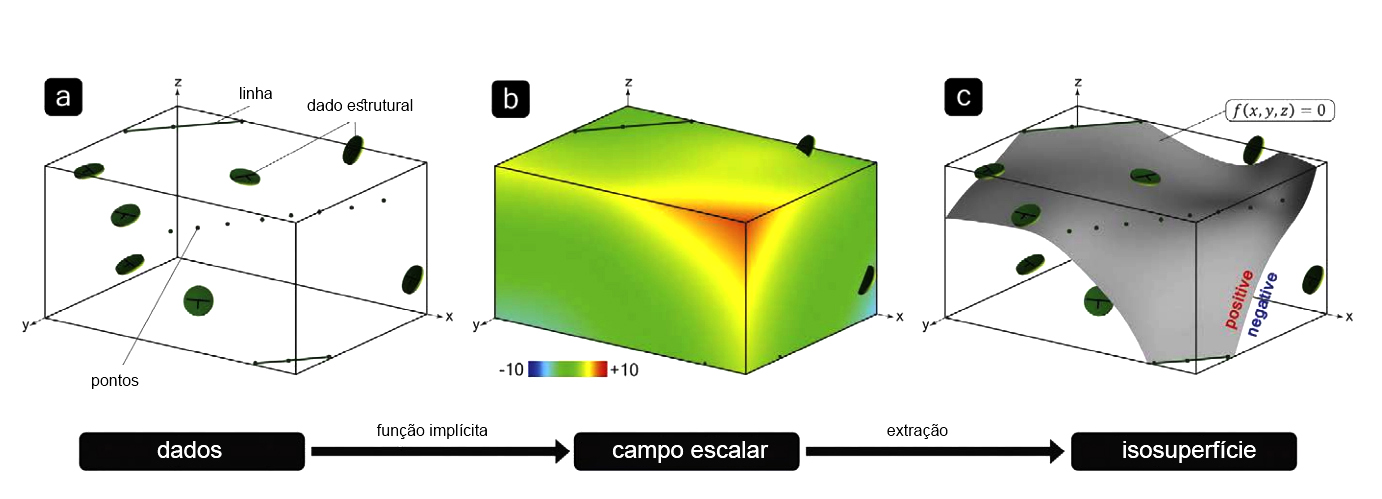
\includegraphics[width=0.8\textwidth]{capitulo_1/implicit_modelig_pt_1}
			\caption{Esquema dos métodos implícitos.}
		\end{center}
	\end{figure}

\begin{itemize}
	\item \cite{mallet2004space} propõe uma função volumétrica cronológica, levando em consideração a posição estratigráfica das diferentes unidades geológicas;
	\item \cite{lajaunie1997foliation} usam co-krigagem de incrementos em um campo potencial, omitindo a função volume.
\end{itemize}

\end{frame}


\section{Modelagem geológica implícita com funções distância assinaladas}

\subsection{O banco de dados}

\begin{frame}{O banco de dados}

72 furos totalizando 3349 amostras distribuídas entre 3 diferentes categorias.

	\begin{figure}
		\centering
		\subfloat[Proporções.]{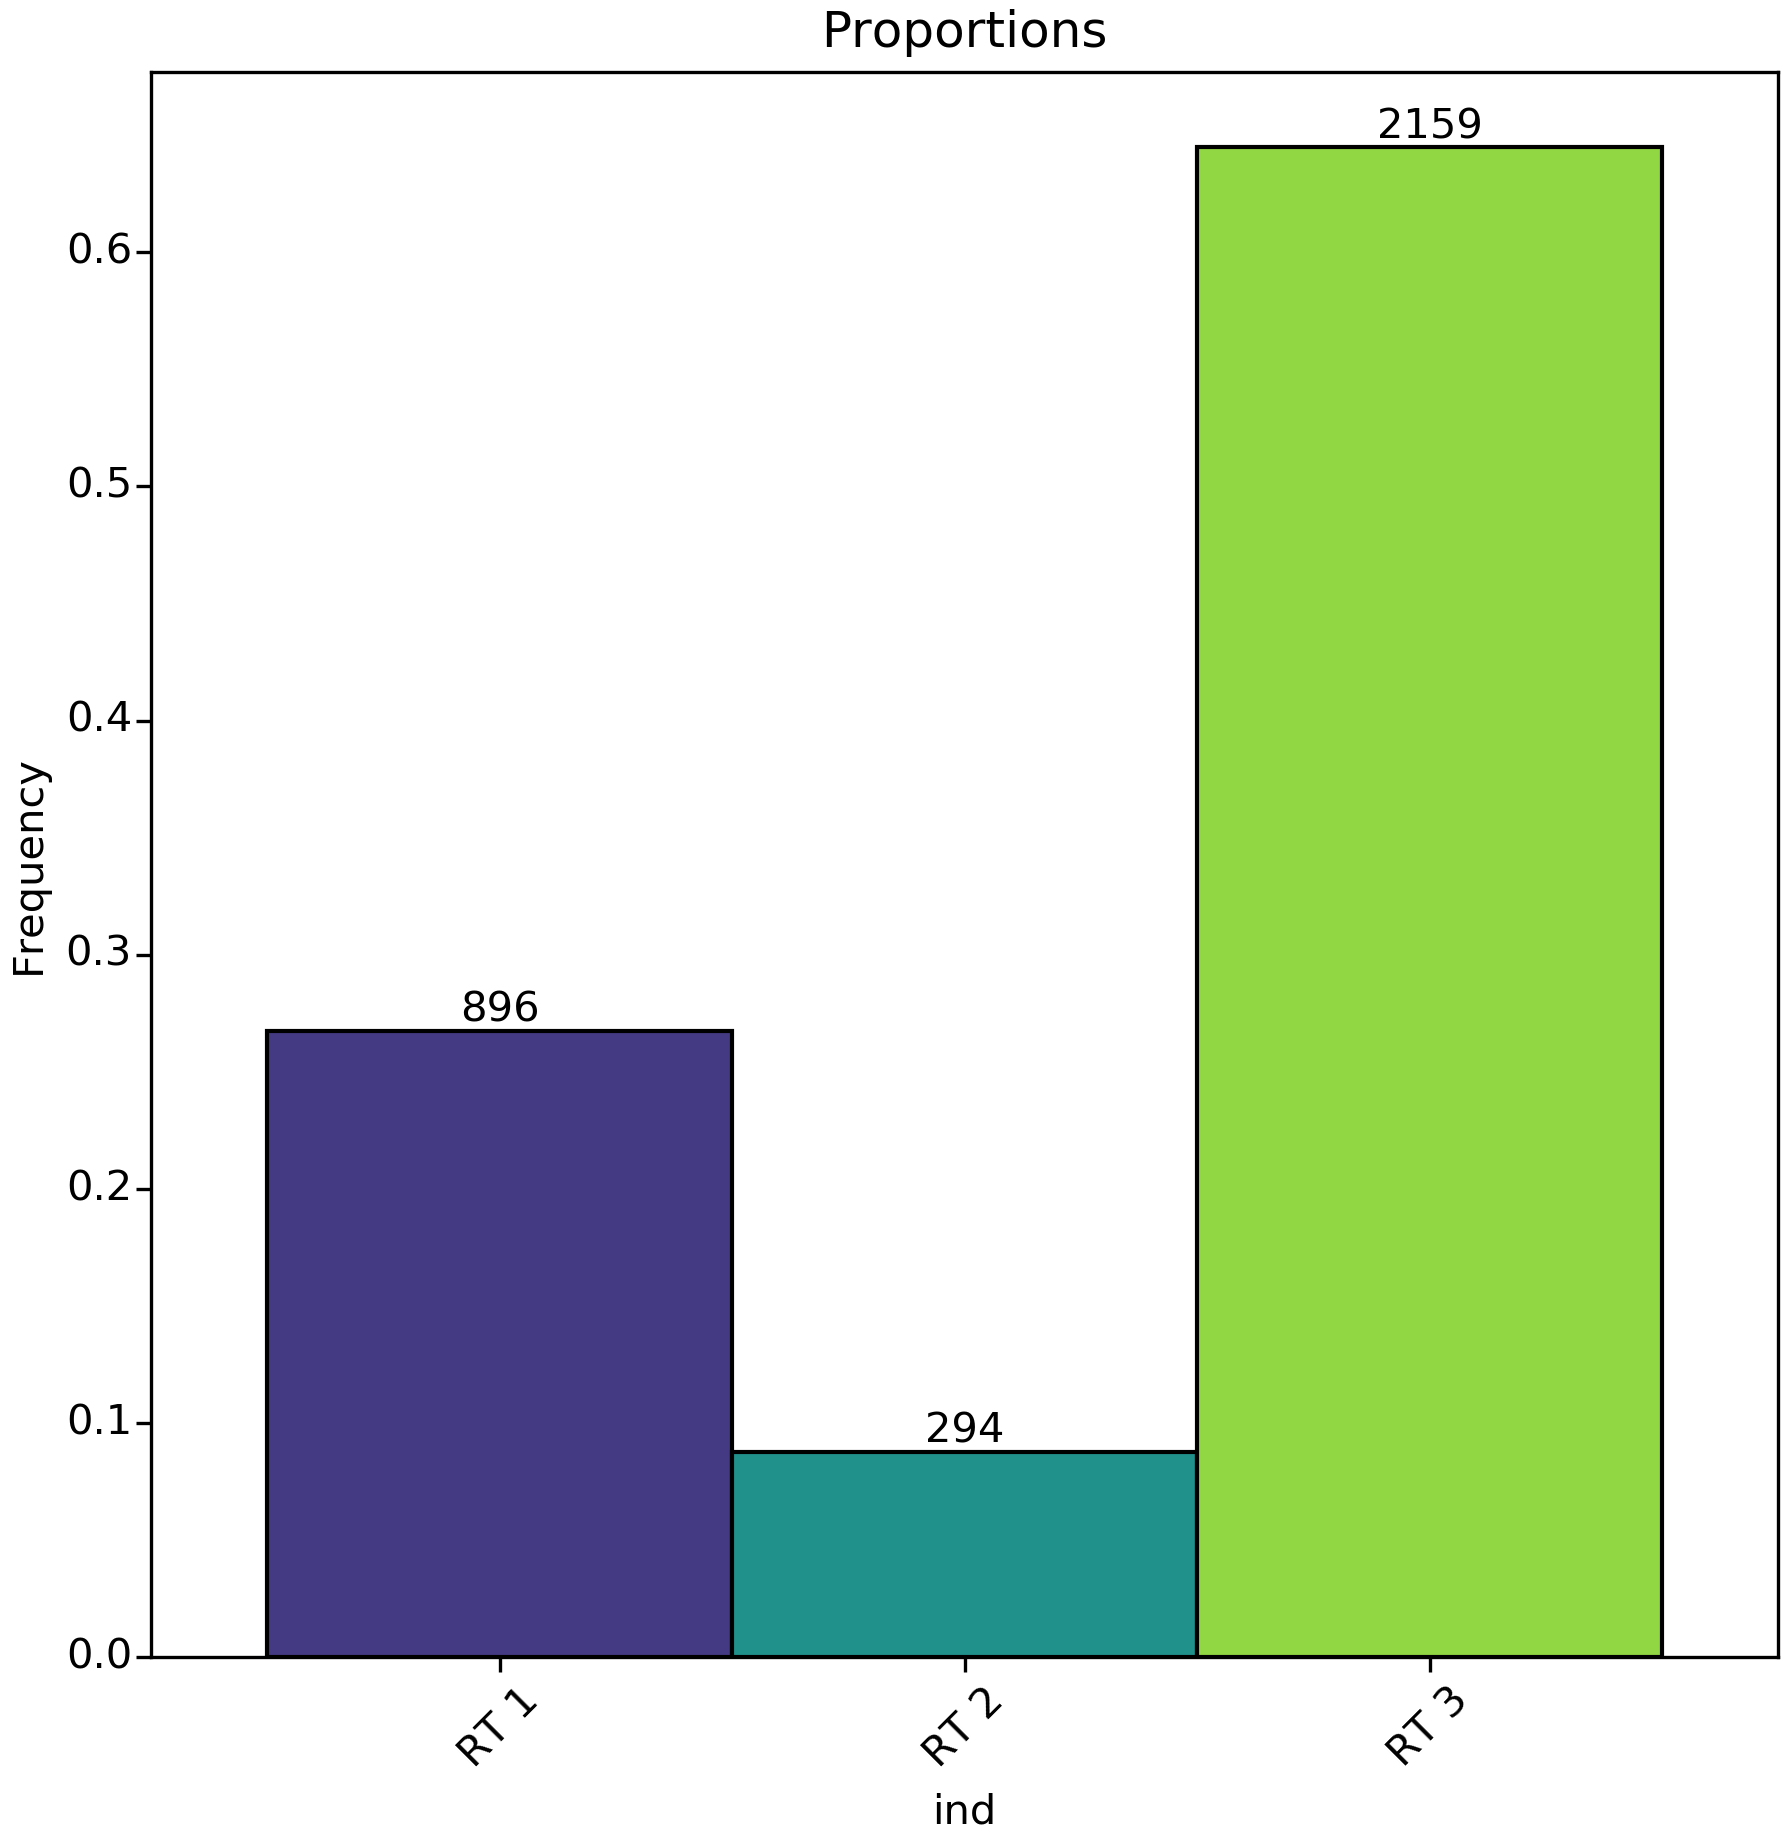
\includegraphics[width=.25\textwidth]{capitulo_2/prop_hist_big.png}}\hspace{20mm}
		\subfloat[Vista das amostras.]{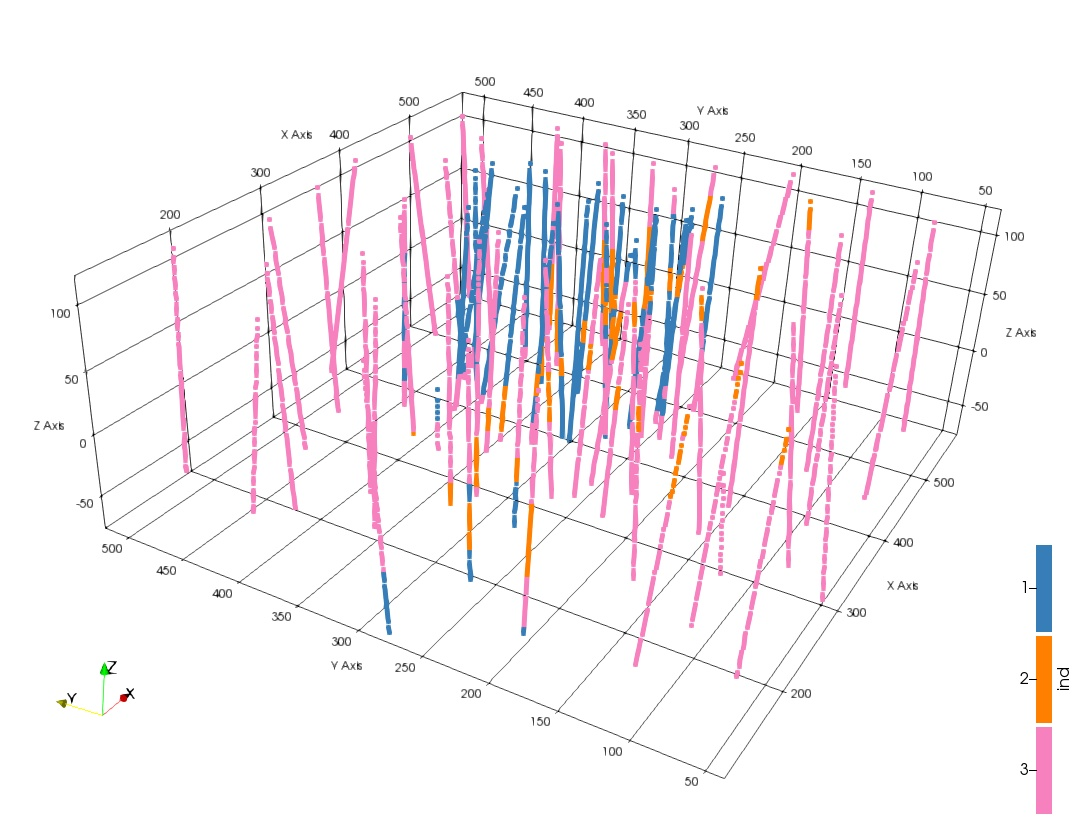
\includegraphics[width=.4\textwidth]{capitulo_2/dados.jpeg}}
		\caption{O banco de dados.}
	\end{figure}
		
\end{frame}

\subsection{Codificando as amostras em indicadores}

\begin{frame}{Codificando as amostras em indicadores}
	\begin{equation}
	i_k(u_\alpha)=\begin{cases}
	1,\:\textrm{se}\:z(u_\alpha)\:\textrm{se pertence ao domínio $k$}\\
	0,\:\textrm{se}\:z(u_\alpha)\:\textrm{caso contrário}\end{cases}
	\label{eq_ind}
	\end{equation}
	
	\begin{figure}[H]
		\caption{Amostras codificadas em indicadores para cada uma das três categorias do banco de dados.} \label{ind}
		\centering
		\subfloat[][Categoria 1]{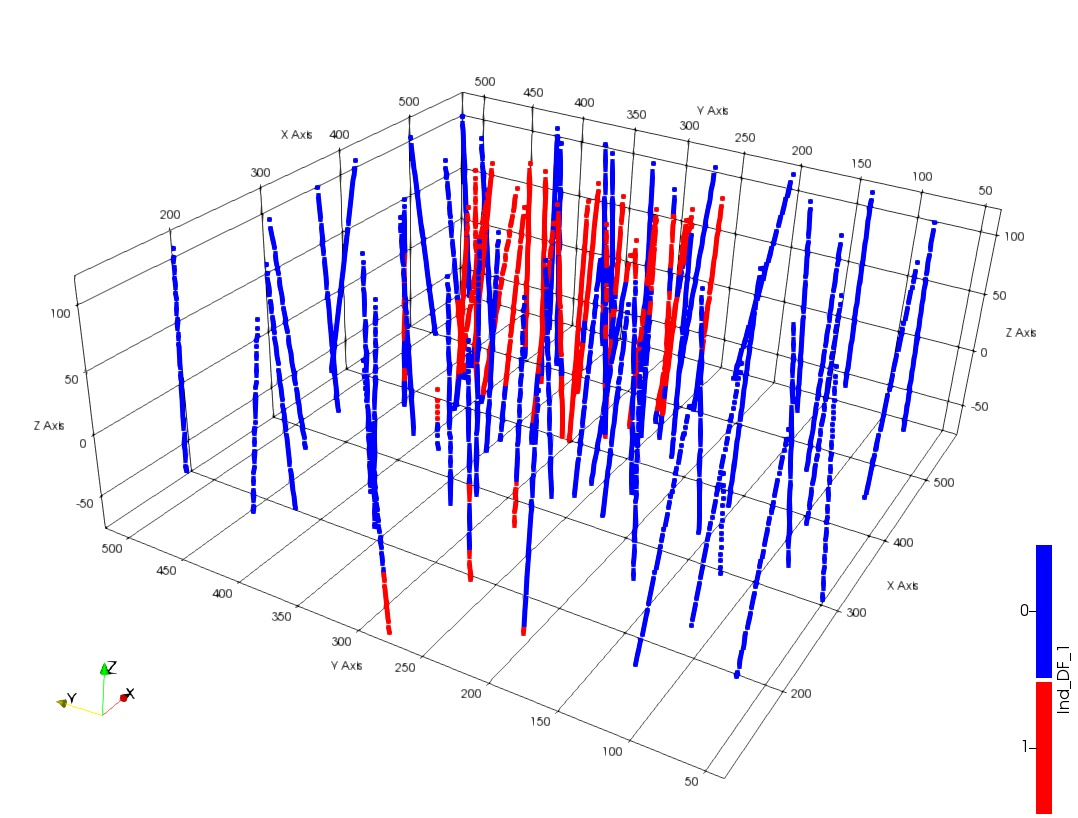
\includegraphics[width=.3\textwidth]{capitulo_2/inddf1.jpeg}\label{<figure1>}}
		\subfloat[][Categoria 2]{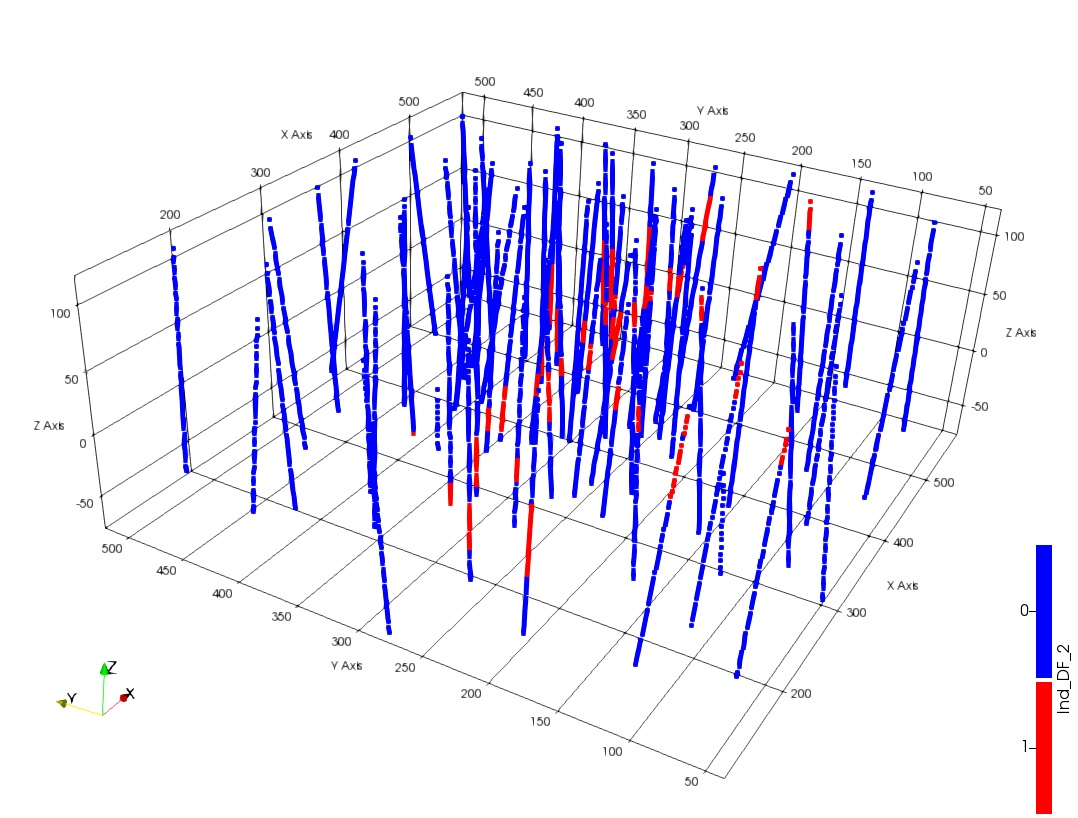
\includegraphics[width=.3\textwidth]{capitulo_2/inddf2.jpeg}\label{<figure2>}}
		\subfloat[][Categoria 3]{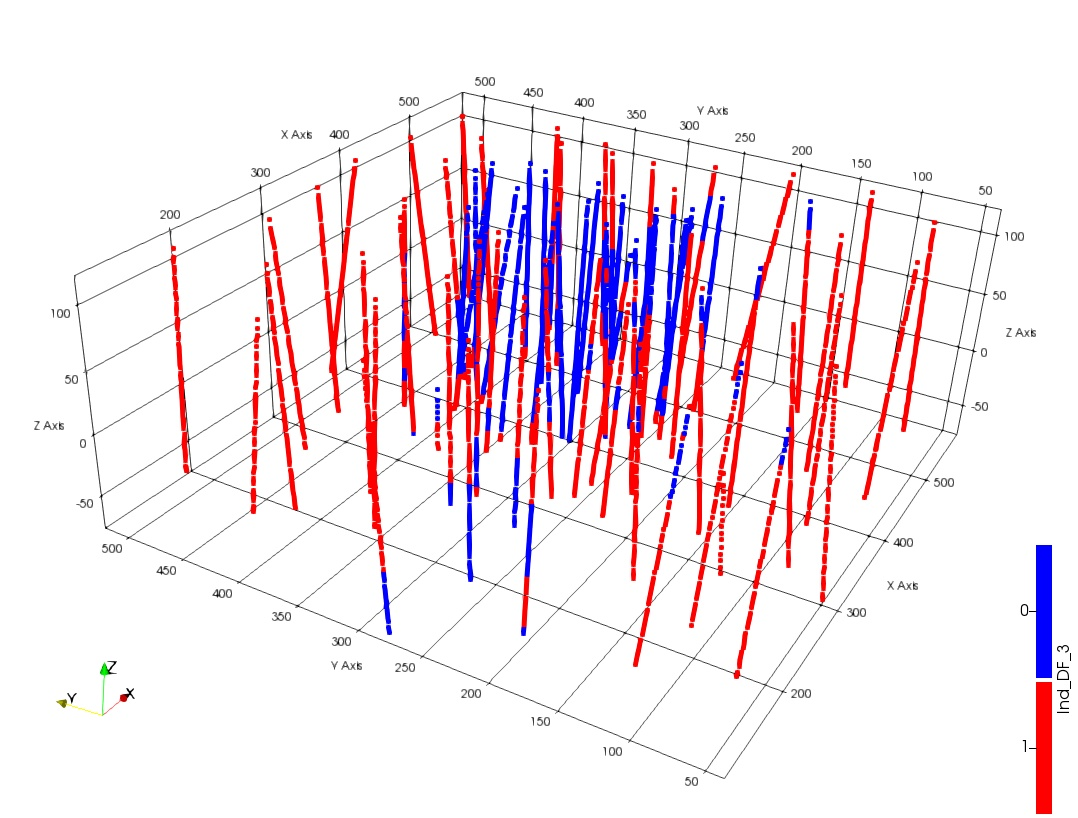
\includegraphics[width=.3\textwidth]{capitulo_2/inddf3.jpeg}\label{<figure2>}}
	\end{figure}
\end{frame}

\subsection{Calculando a função distância assinalada}

\begin{frame}{Calculando a função distância assinalada}

\begin{equation}
d_k(u_\alpha)=\begin{cases}
-\parallel u_\alpha-u_\beta\parallel,\:\textrm{se $u_\alpha$ pertence ao domínio}\\
+\parallel u_\alpha-u_\beta\parallel,\:\textrm{se $u_\alpha$ não pertence ao domínio}\end{cases}
\label{eq_mult_sg}
\end{equation}

O local $u_\beta$ corresponde à amostra mais próxima codificada com um indicador diferente de $u_\alpha$.
\begin{figure}[H]
	\caption{\label{2d_ex}Ilustração esquemática mostrando o cálculo das distâncias assinaladas.}
	\begin{center}
		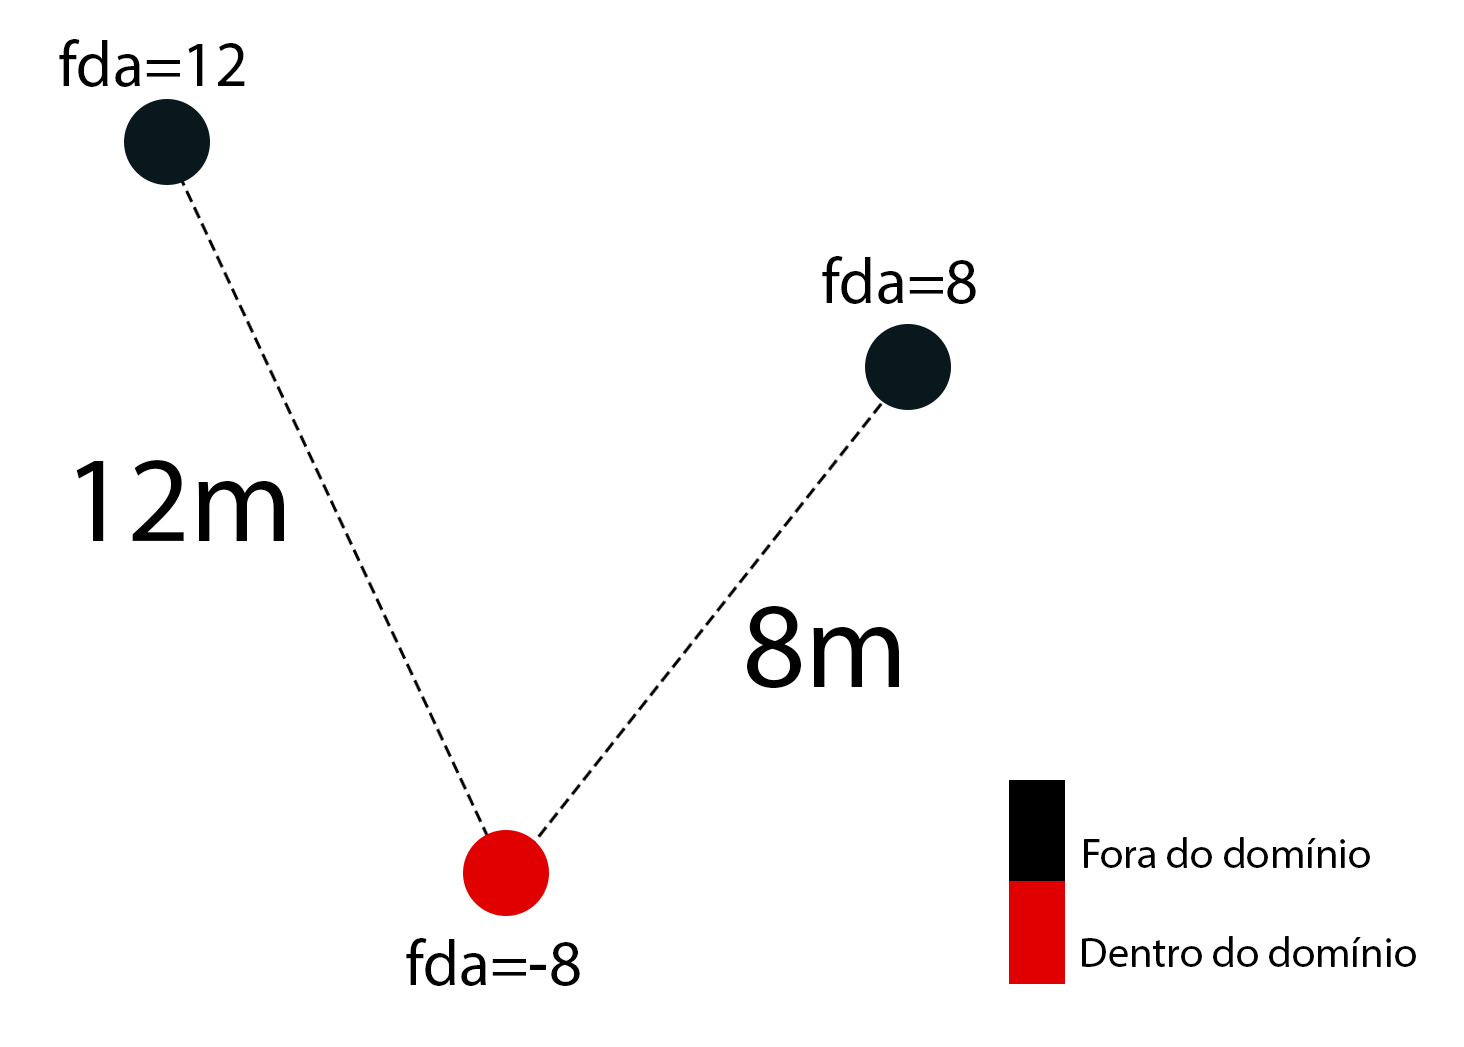
\includegraphics[width=0.3\textwidth]{capitulo_2/2d_ex.jpg}
	\end{center}
	%\legend{Modificado de \citeonline{martin2017implicitmodeling}}
\end{figure}
\end{frame}

\begin{frame}{Calculando a função distância assinalada} 
	\begin{figure}[H]
		\caption{Distâncias assinaladas calculadas para cada uma das categorias do banco de dados.} \label{indcalc}
		\centering
		\subfloat[][Categoria 1]{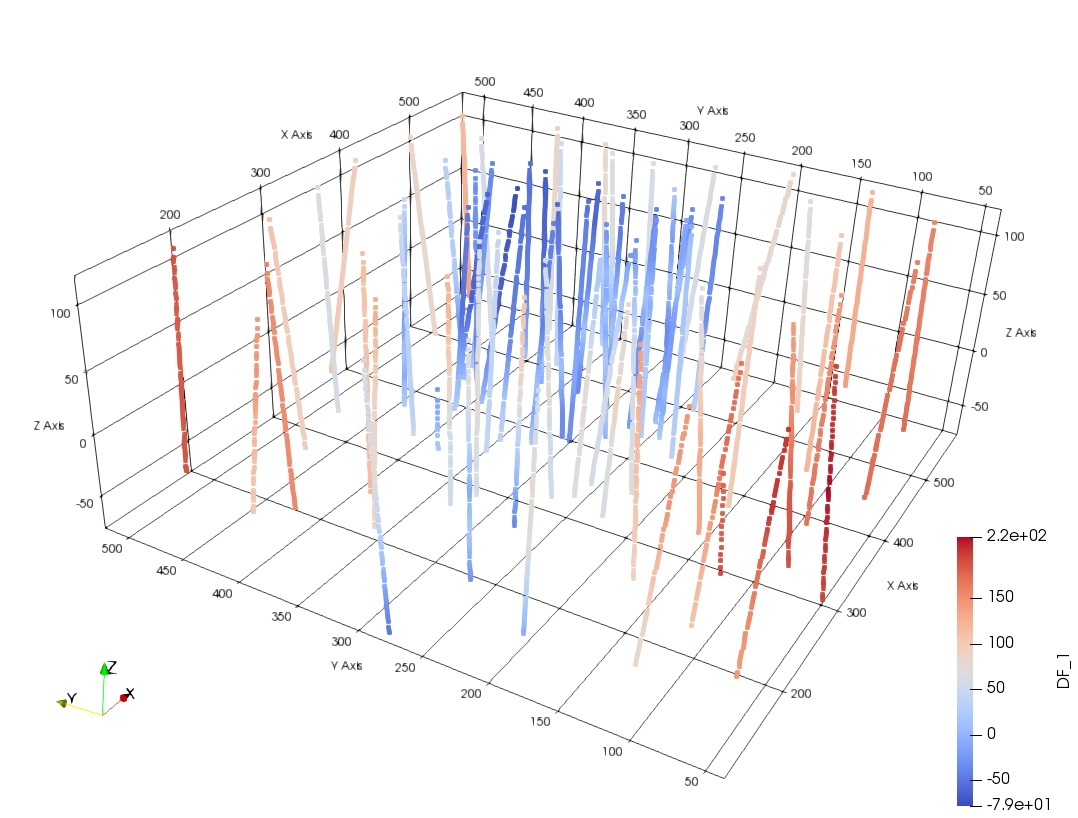
\includegraphics[width=.3\textwidth]{capitulo_2/df1.jpeg}\label{<figure1>}}
		\subfloat[][Categoria 2]{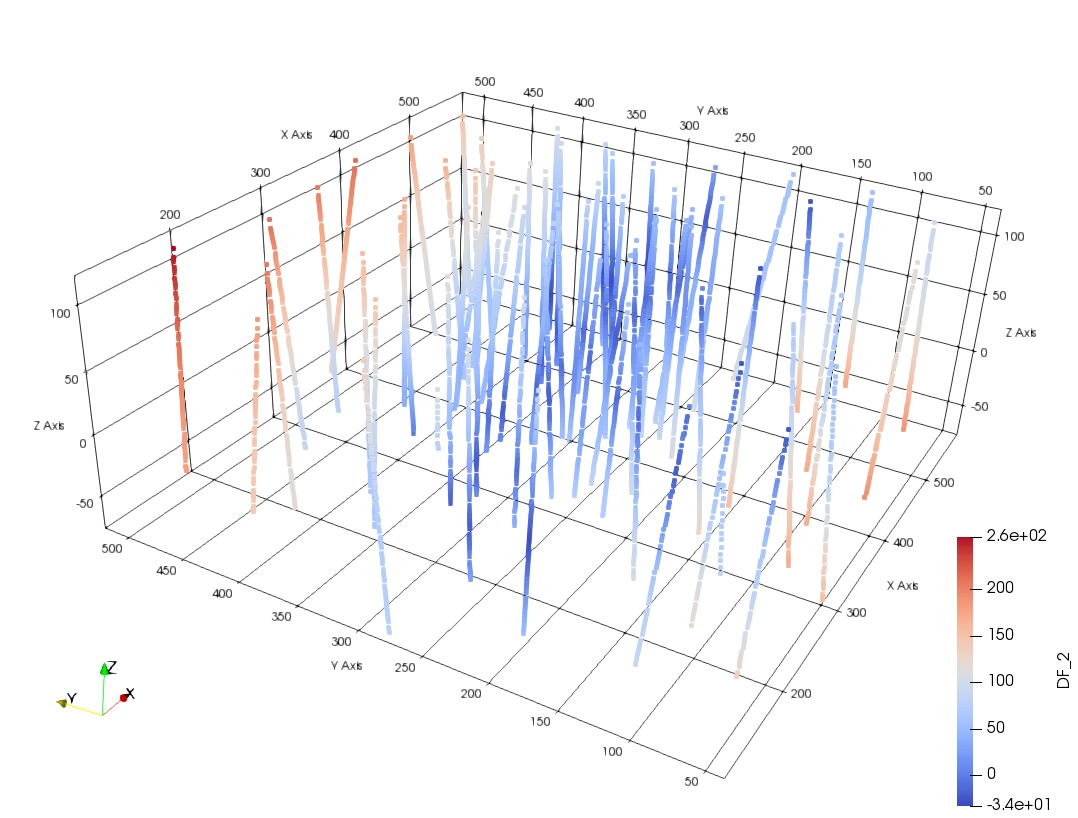
\includegraphics[width=.3\textwidth]{capitulo_2/df2.jpeg}\label{<figure2>}}
		\subfloat[][Categoria 3]{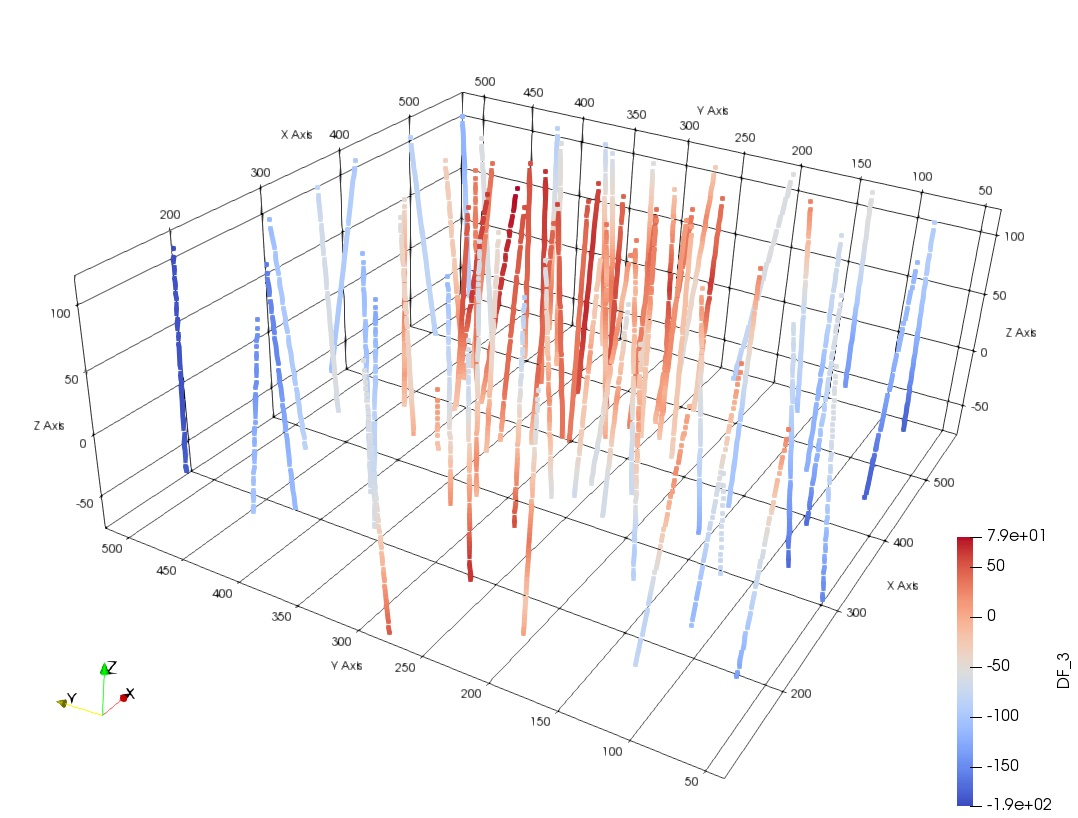
\includegraphics[width=.3\textwidth]{capitulo_2/df3.jpeg}\label{<figure2>}}
	\end{figure}
\end{frame}

\subsection{Variografia das distâncias assinaladas}

\begin{frame}{Variografia das distâncias assinaladas}

Distâncias assinaladas não são estacionárias, o variograma não se estabiliza em um patamar. Além disso, o caráter extremamente contínuo das distâncias torna a identificação analítica das direções principais um processo embaraçoso.

\begin{itemize}
	\item Treinar o variograma usando validação cruzada;
	\item Tentar modelar interativamente os variogramas experimentais;
	\item Calcular e modelar os variogramas para as propriedades de indicadores e transformá-los em um equivalente gaussiano para as distâncias assinaladas;
	\item inferir um modelo de covariância plausível visualmente a partir das amostras ou de mapas delineados a mão.
\end{itemize}
\end{frame}

\begin{frame}{Variogramas das distâncias assinaladas}
\begin{figure}[H] 
	\caption{Variogramas experimentais das distâncias assinaladas e modelos para cada uma das categorias do banco de dados.} \label{sd_var}
	\centering
	\subfloat[][Categoria 1]{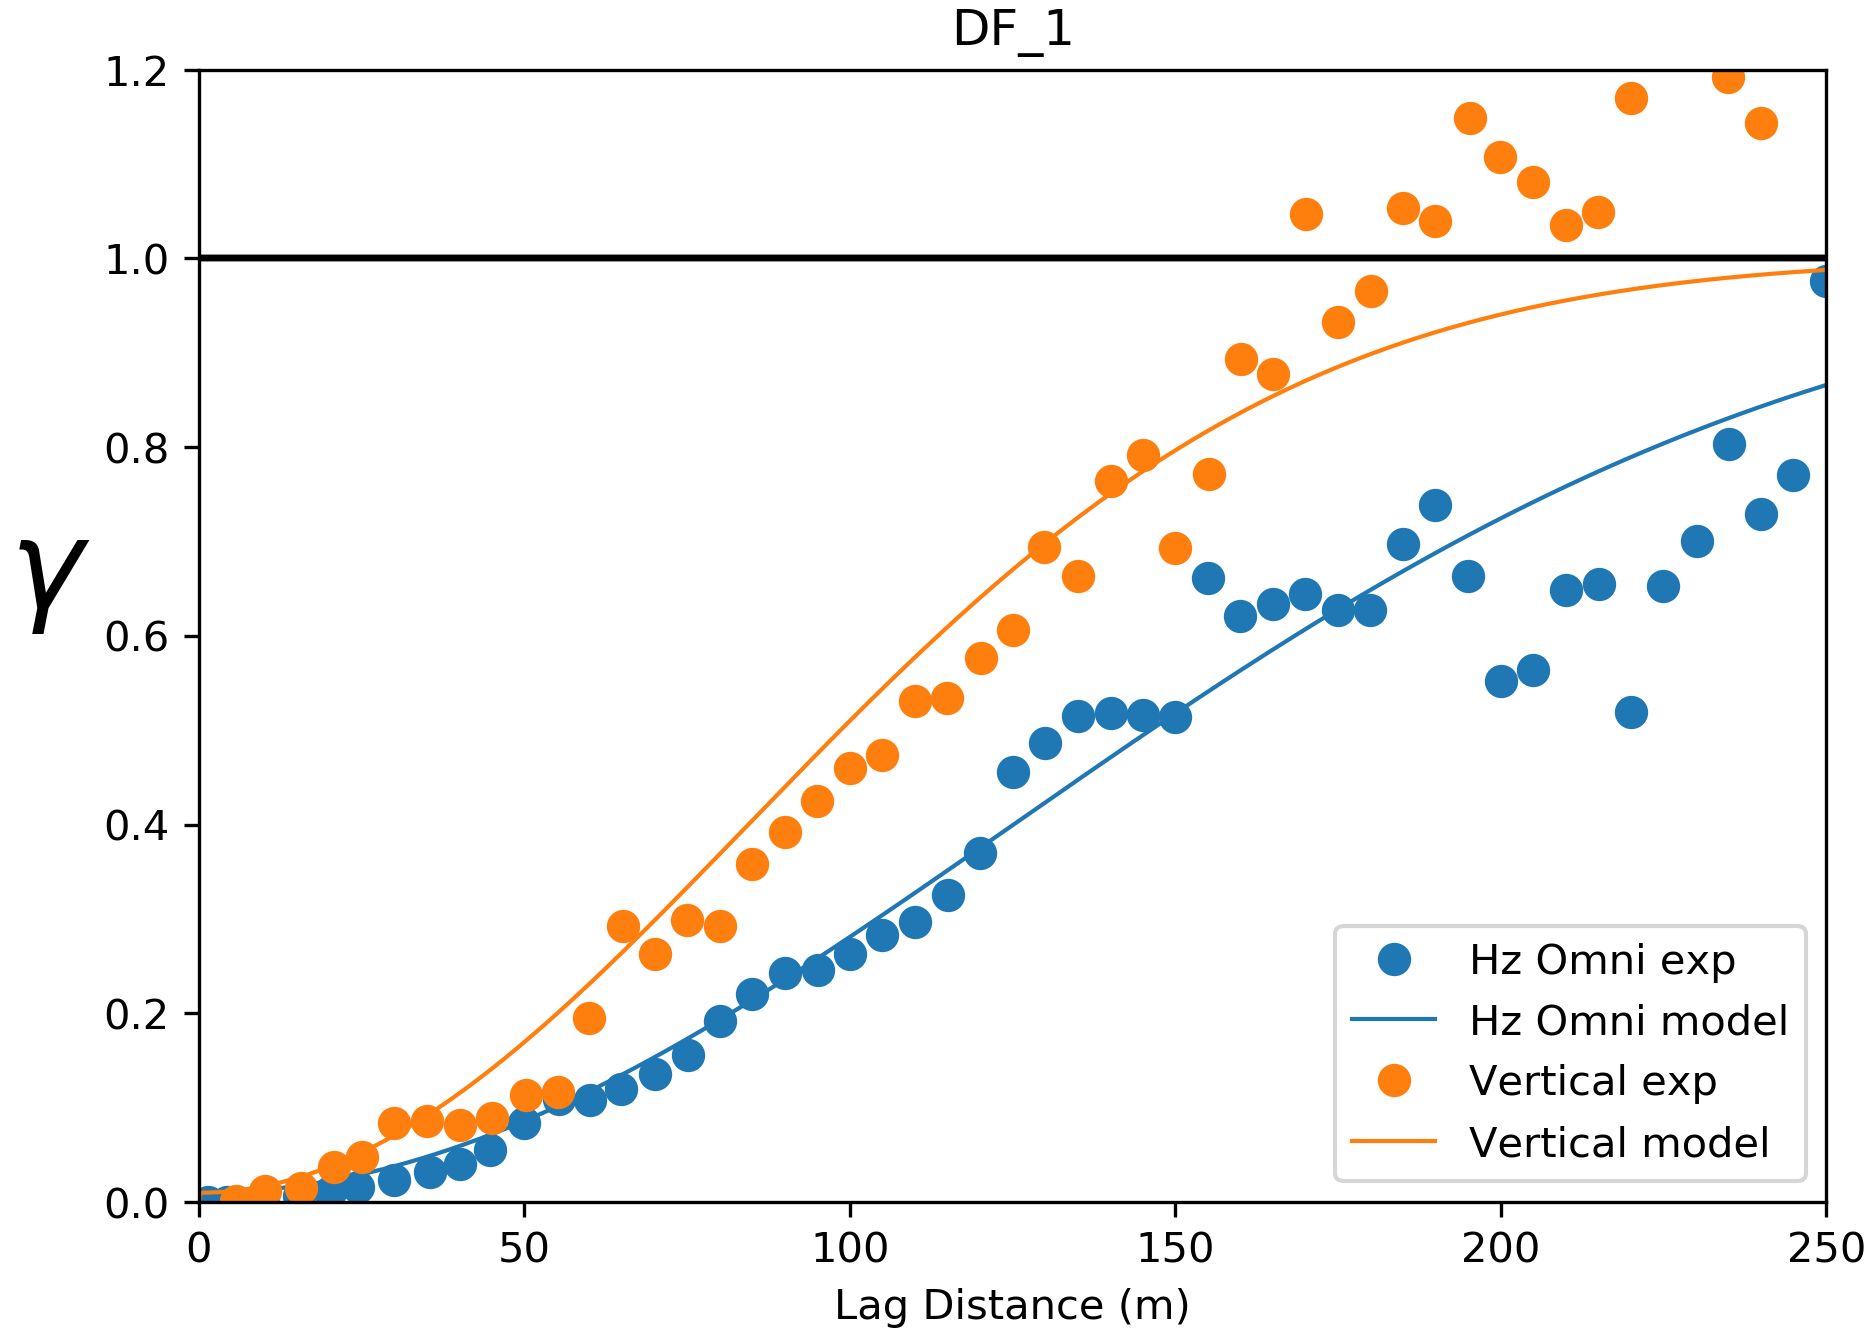
\includegraphics[width=.3\textwidth]{capitulo_2/var_DF_1.png}\label{<figure1>}}
	\subfloat[][Categoria 2]{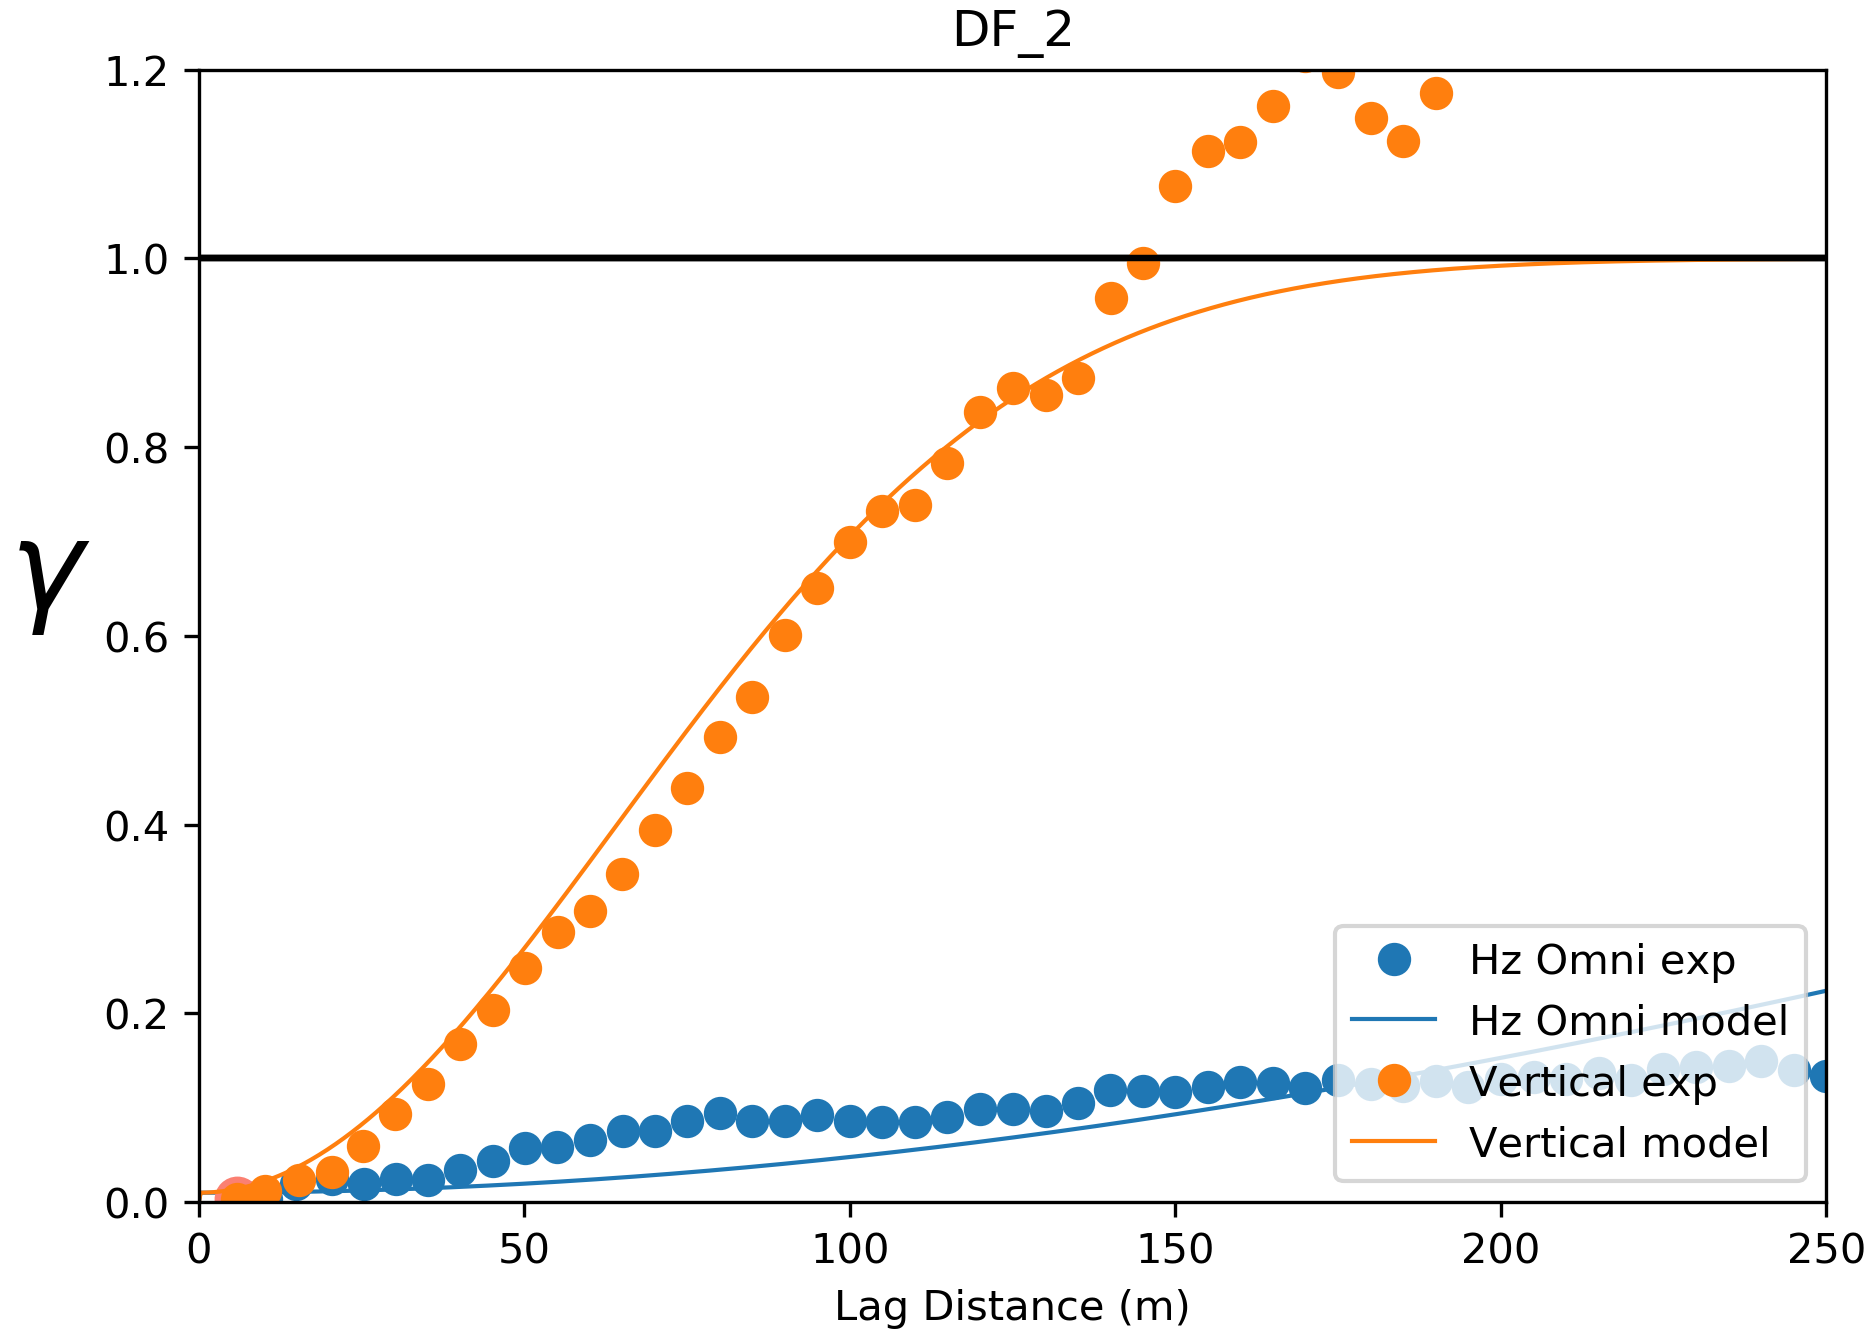
\includegraphics[width=.3\textwidth]{capitulo_2/var_DF_2.png}\label{<figure2>}}
	\subfloat[][Categoria 3]{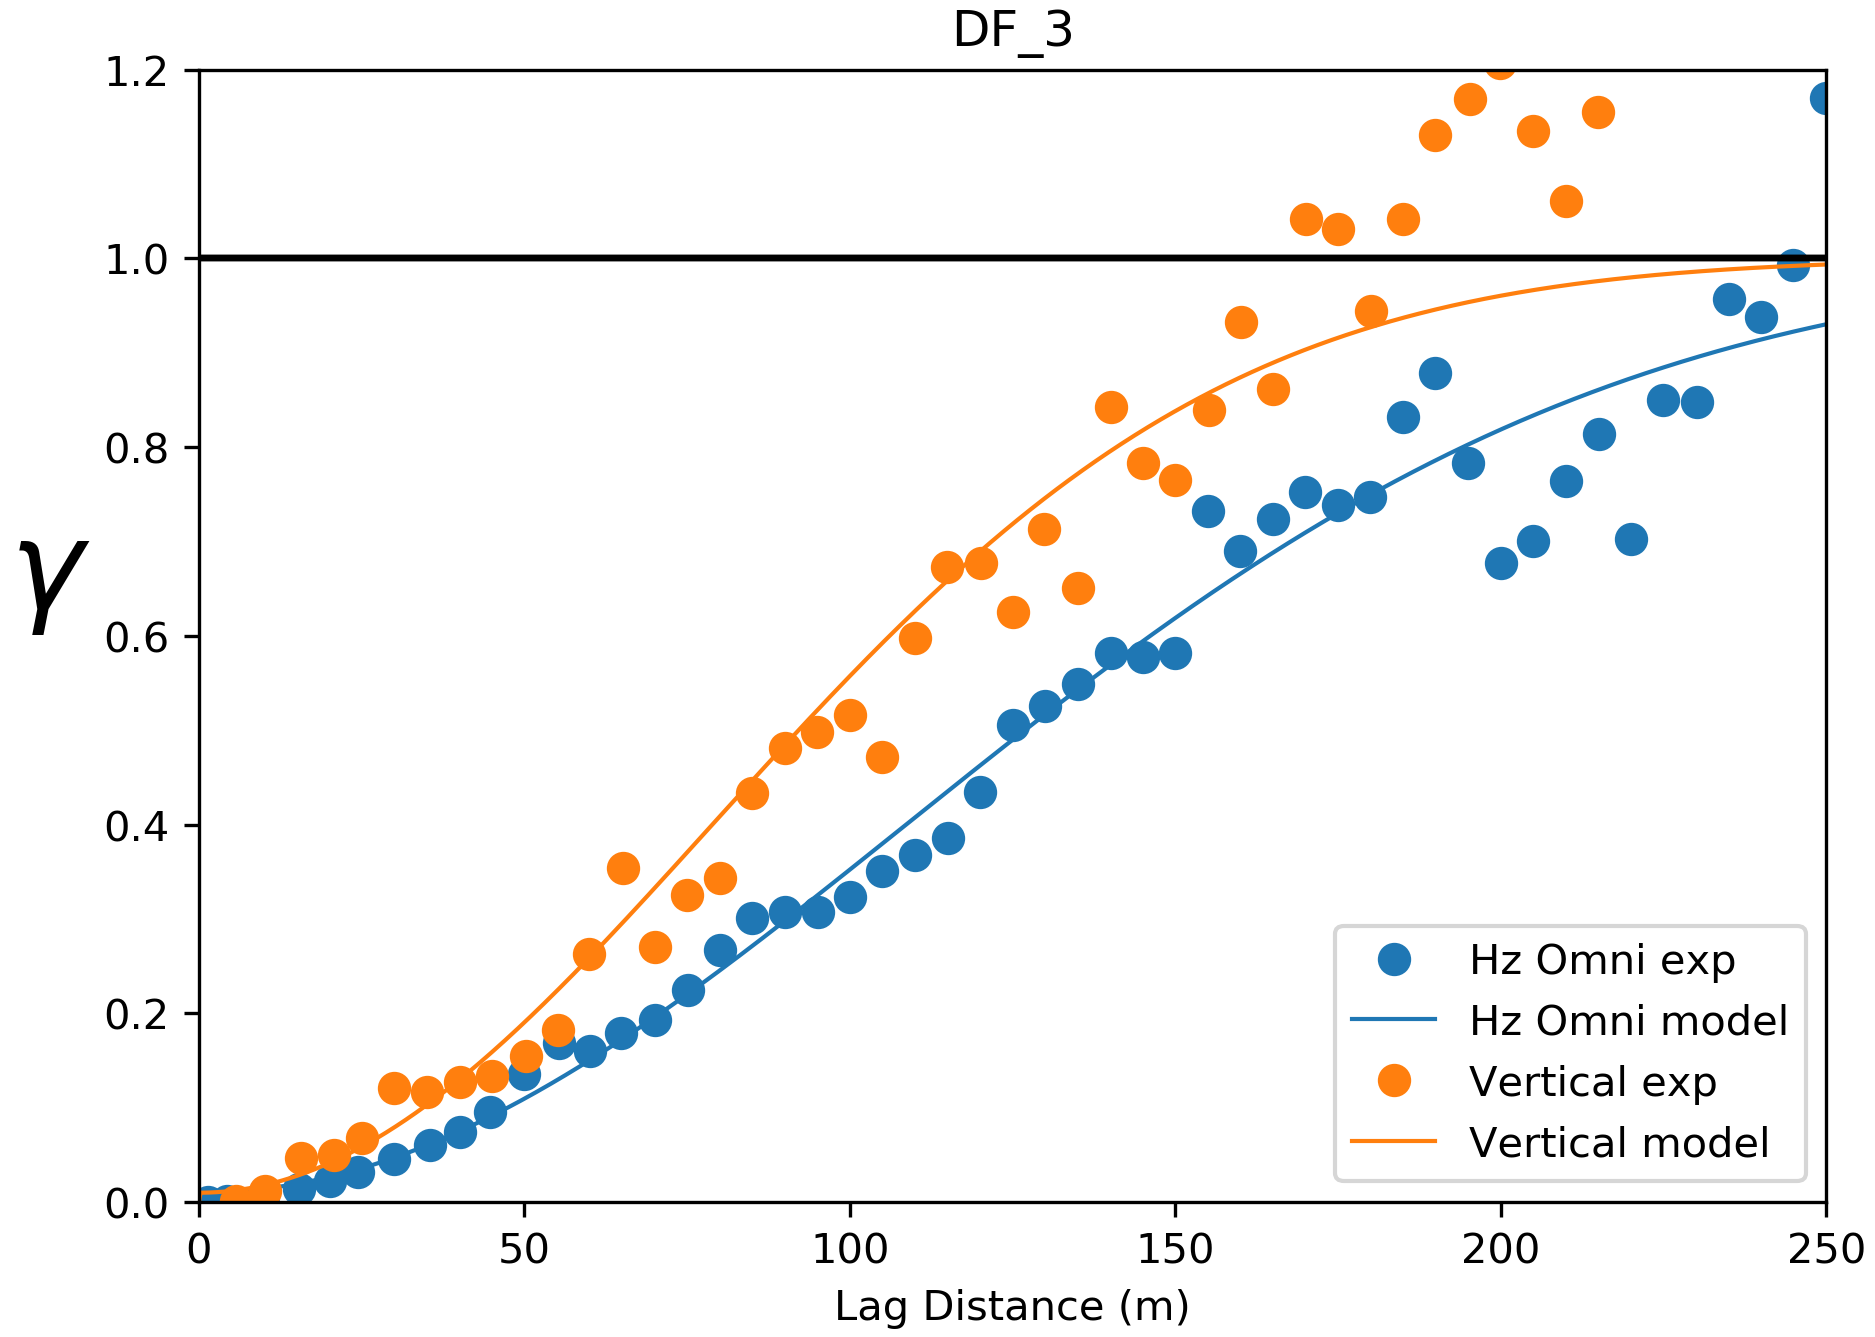
\includegraphics[width=.3\textwidth]{capitulo_2/var_DF_3.png}\label{<figure2>}}
\end{figure}
\end{frame}

\begin{frame}{Variogramas dos indicadores}
	\begin{figure}[H] 
		\caption{Variogramas experimentais dos indicadores e modelos para cada uma das categorias do banco de dados.} \label{ind_var}
		\centering
		\subfloat[][Categoria 1]{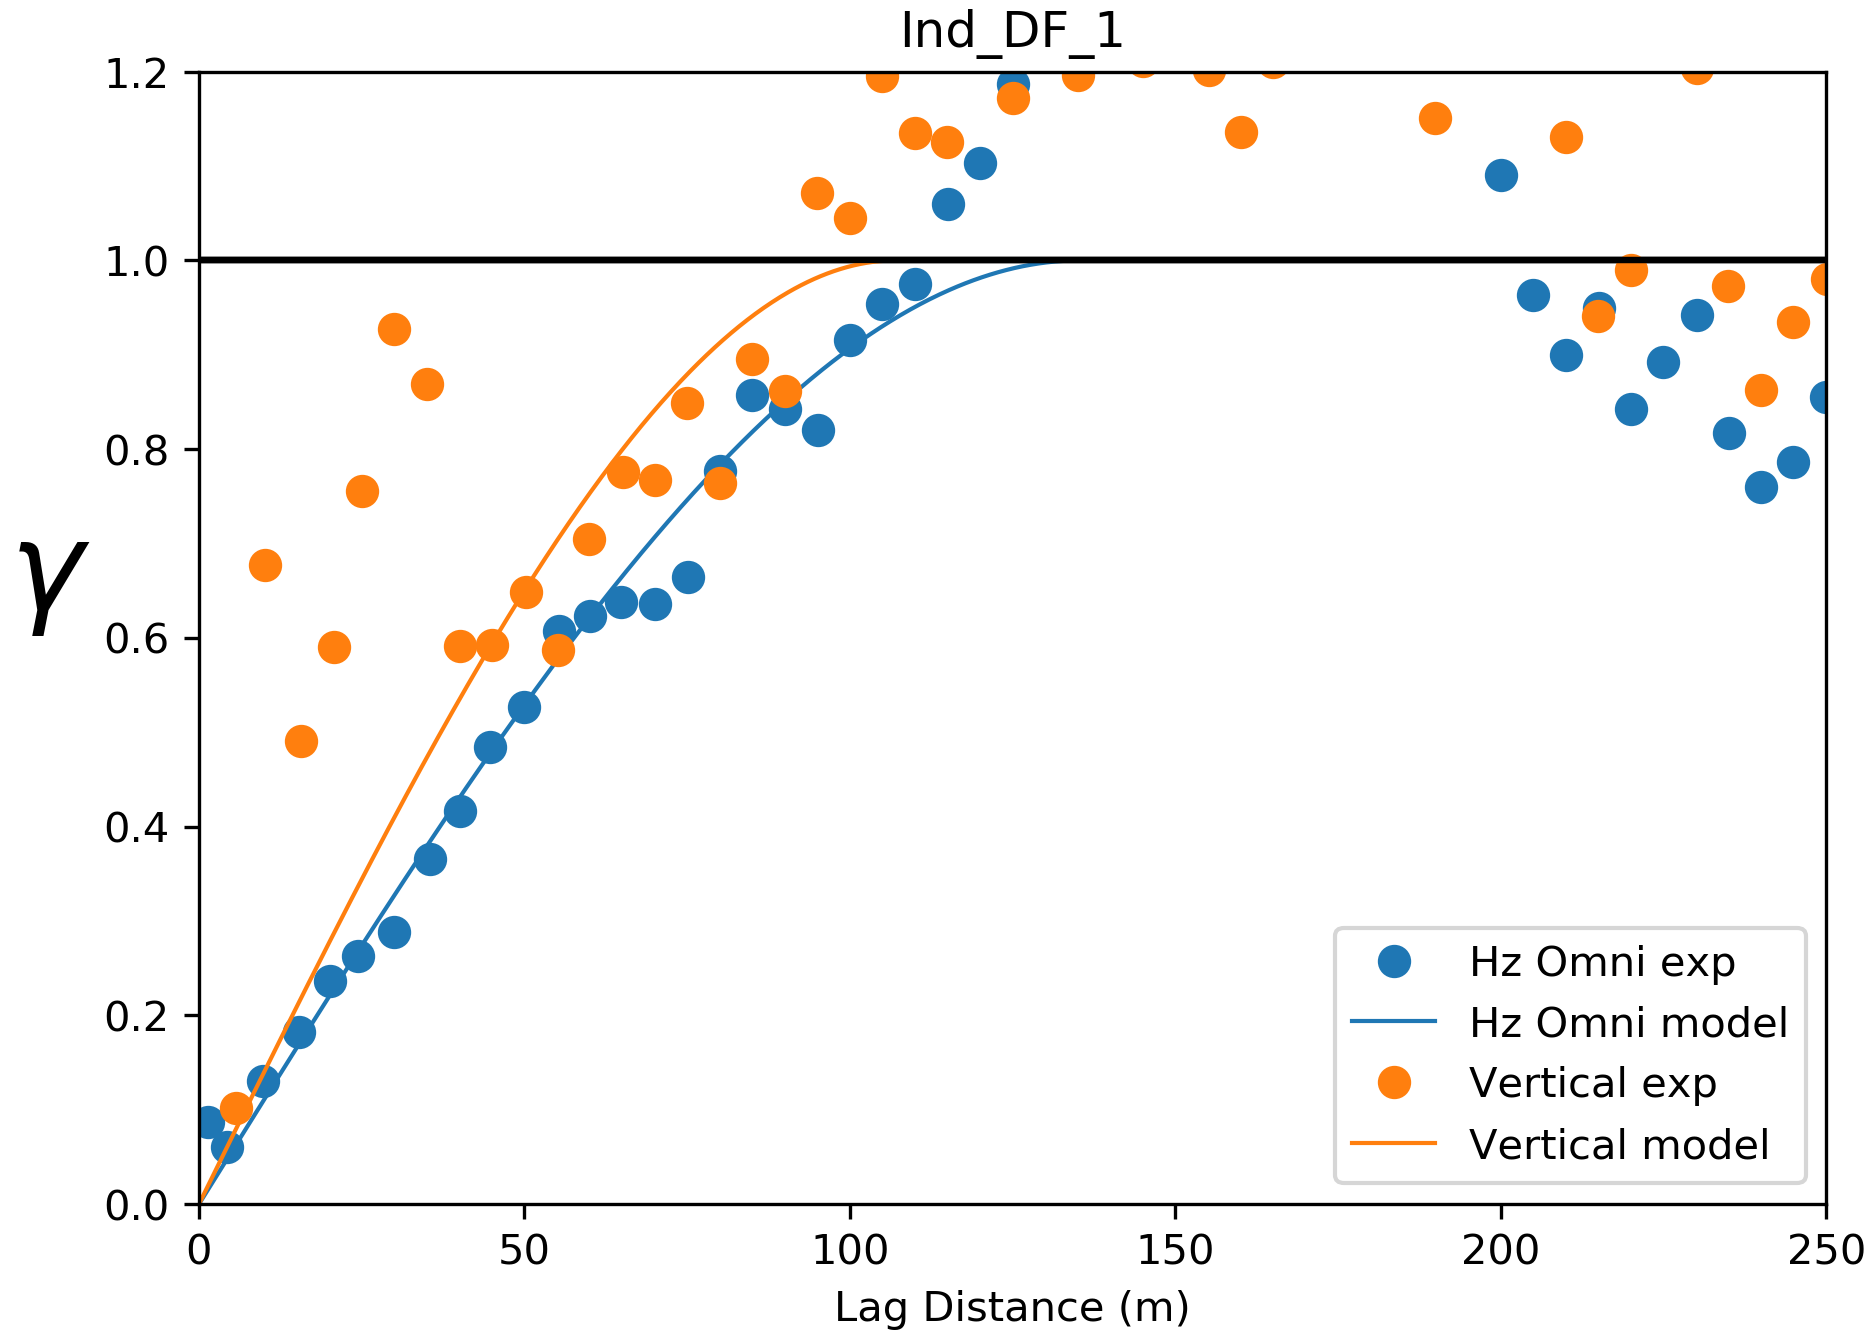
\includegraphics[width=.3\textwidth]{capitulo_2/var_Ind_DF_1.png}\label{<figure1>}}
		\subfloat[][Categoria 2]{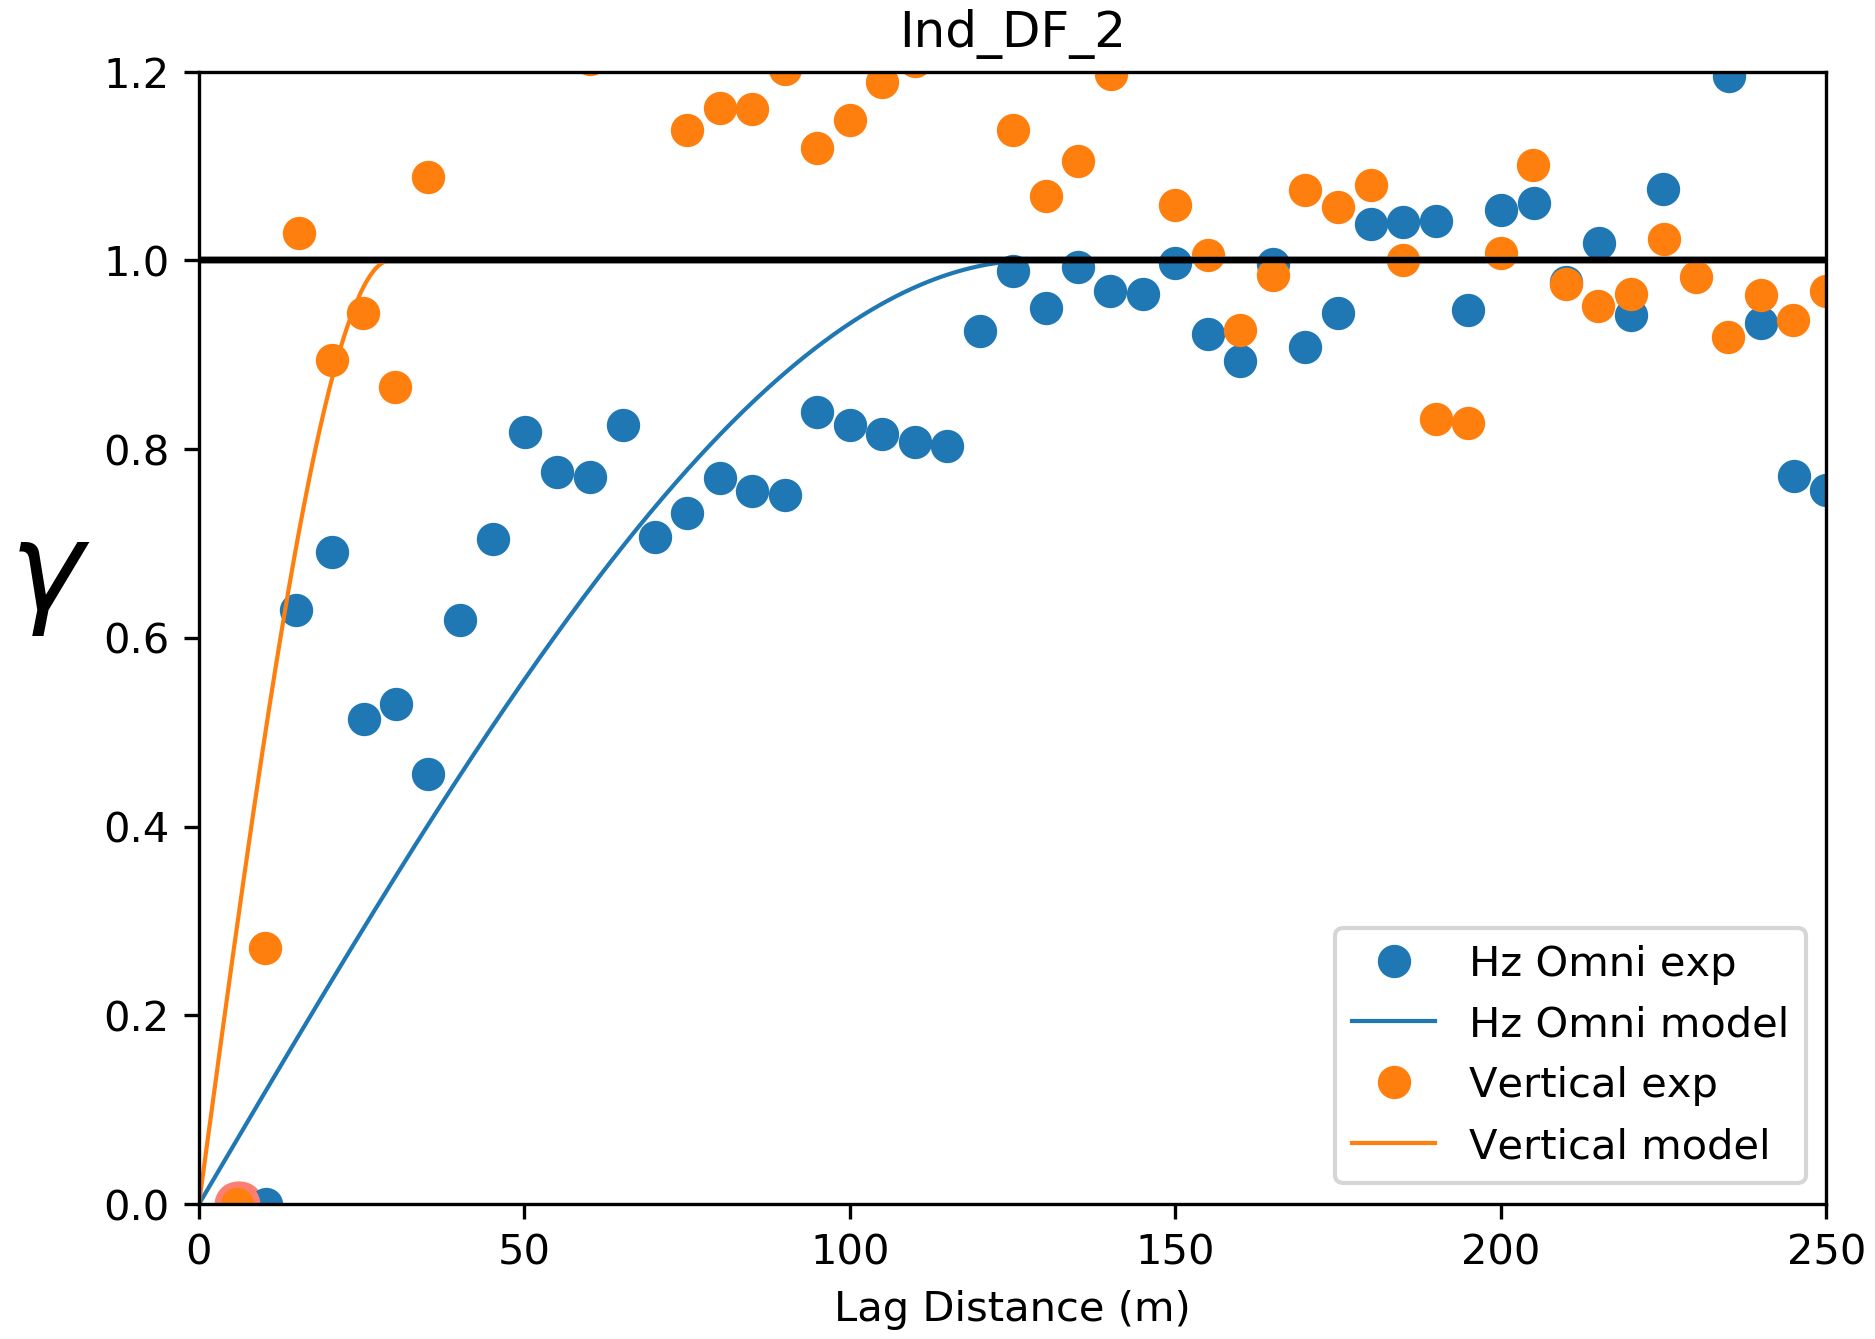
\includegraphics[width=.3\textwidth]{capitulo_2/var_Ind_DF_2.png}\label{<figure2>}}
		\subfloat[][Categoria 3]{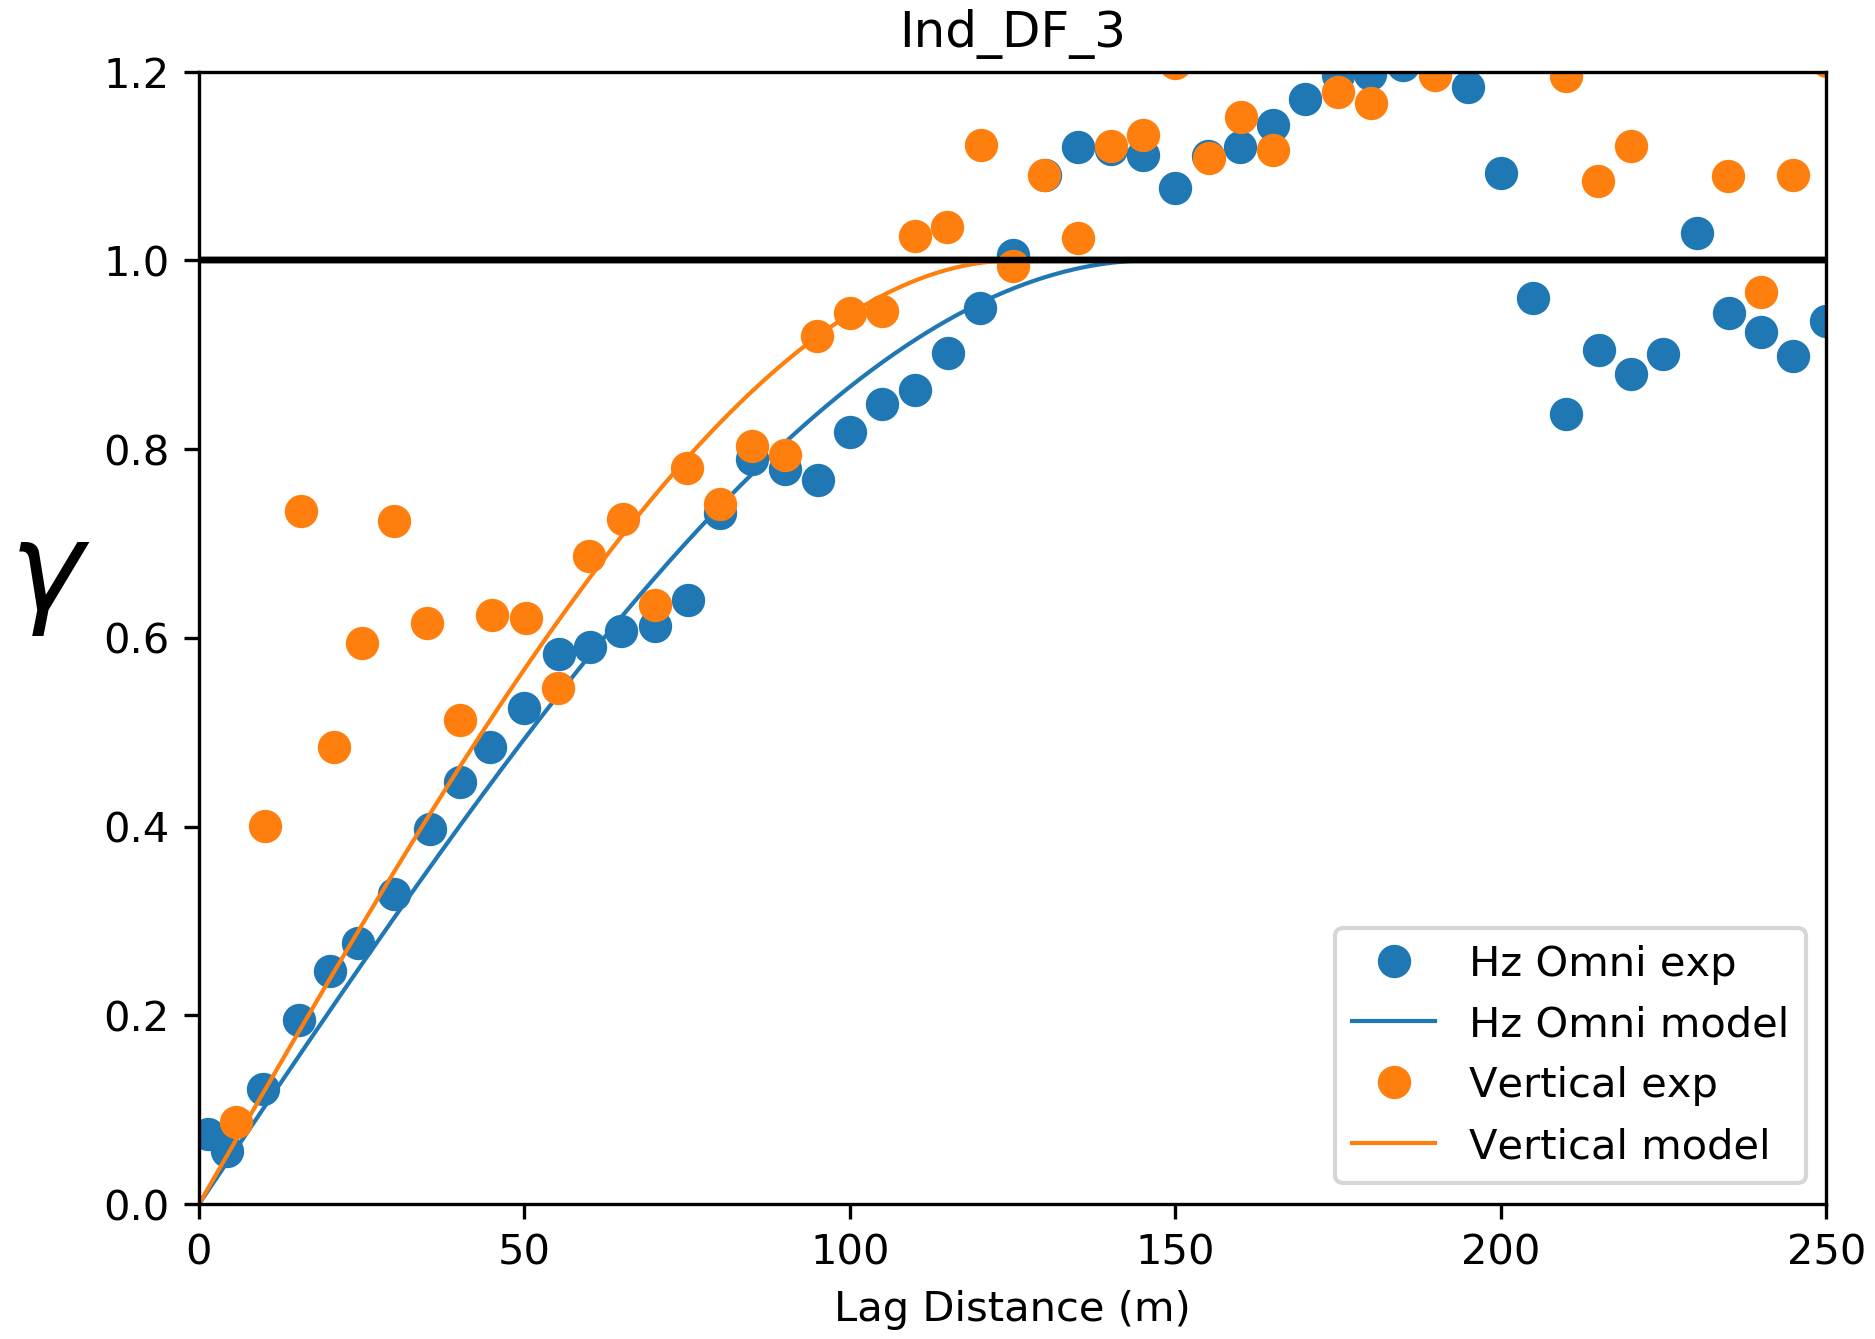
\includegraphics[width=.3\textwidth]{capitulo_2/var_Ind_DF_3.png}\label{<figure2>}}
	\end{figure}
\end{frame}

\begin{frame}{Alternativa ao cálculo e modelagem dos variogramas}
	\begin{figure}[H]
		\caption{\label{cov_table}Fluxograma da modelagem geológica implícita usando tabelas de covariância.}
		\begin{center}
			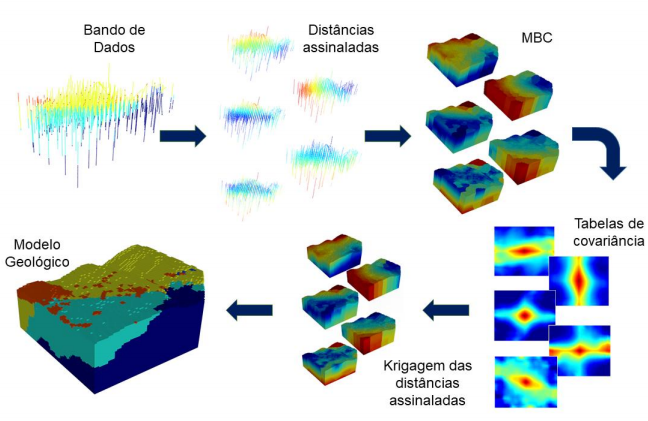
\includegraphics[width=0.7\textwidth]{capitulo_2/cov_table.png}
		\end{center}
		%\legend{\citeonline{kloechner_cov_table}}
	\end{figure}
\end{frame}

\subsection{Interpolação das distâncias assinaladas}

\begin{frame}{Resolução do grid}

\begin{figure}[H]
	\caption{\label{grid_res}Efeito da resolução do \textit{grid} na reprodução de estruturas geológicas.}
	\begin{center}
		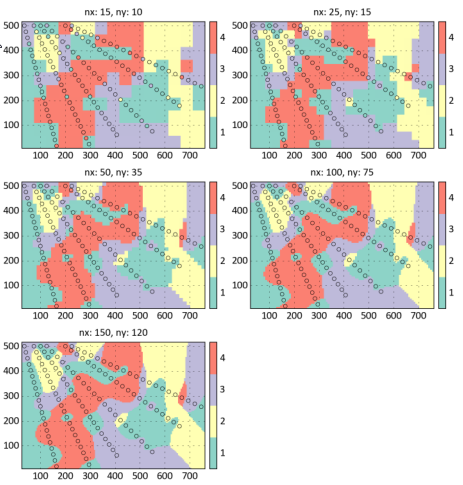
\includegraphics[width=0.4\textwidth]{capitulo_2/grid_res.png}
	\end{center}
	%\legend{Fonte: \citeonline{martin2017implicitmodeling}}
\end{figure}

\end{frame}

\begin{frame}{Grids criados}
	\begin{table}[H]
		\centering
		\begin{tabular}{lrr}
			& \multicolumn{1}{l}{Grosso} & \multicolumn{1}{l}{Fino} \\ \hline
			nx & 49 & 97 \\
			ny & 49 & 98 \\
			nz & 51 & 102 \\
			sx & 10m & 5m \\
			sy & 10m & 5m \\
			sz & 4m & 2m \\
			num & 122451 & 969612 \\ \hline
		\end{tabular}
		\caption{Parâmetros dos \textit{grids} de definição dos modelos geológicos implícitos.} \label{grid_def}
	\end{table}
\end{frame}

\begin{frame}{Métodos de interpolação}
	\begin{itemize}
		\item \cite{hosseini_deutsch_iqd} utilizaram inverso da distância;
		\item \cite{silvaenhancedgeomodeling} utilizou krigagem ordinária global;
		\item \cite{rolo_dissertacao} utilizou krigagem ordinária;
		\item \cite{silva_dual} aplicaram \textit{dual kriging};
		\item \cite{boisvert_geomodeling} gerou modelos implícitos através de distâncias assinaladas com anisotropia variável local (\textit{Locally varying anisotropy kriging - LVA});
		\item \cite{manchuck_MLS} propuseram a utilização de mínimos quadrados móveis para incorporar interpretação manual e avaliar incerteza.
	\end{itemize}
\end{frame}

\begin{frame}{Métodos de interpolação}
	\begin{figure}[H] 
		\caption{Interpolação das distâncias calculadas por diferentes métodos.} \label{interpo}
		\centering
		\subfloat[][OK com 40 amostras]{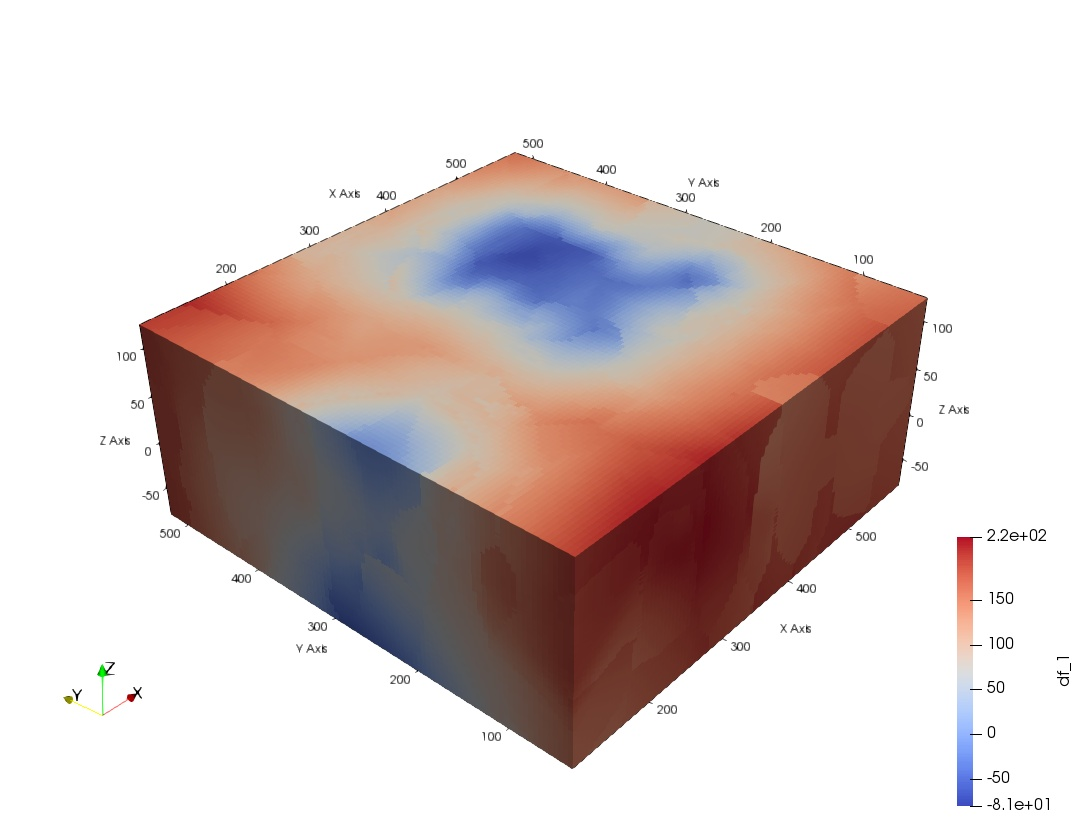
\includegraphics[width=.3\textwidth]{capitulo_2/kt3d40.jpeg}\label{<figure1>}}
		\subfloat[][OK com 100 amostras]{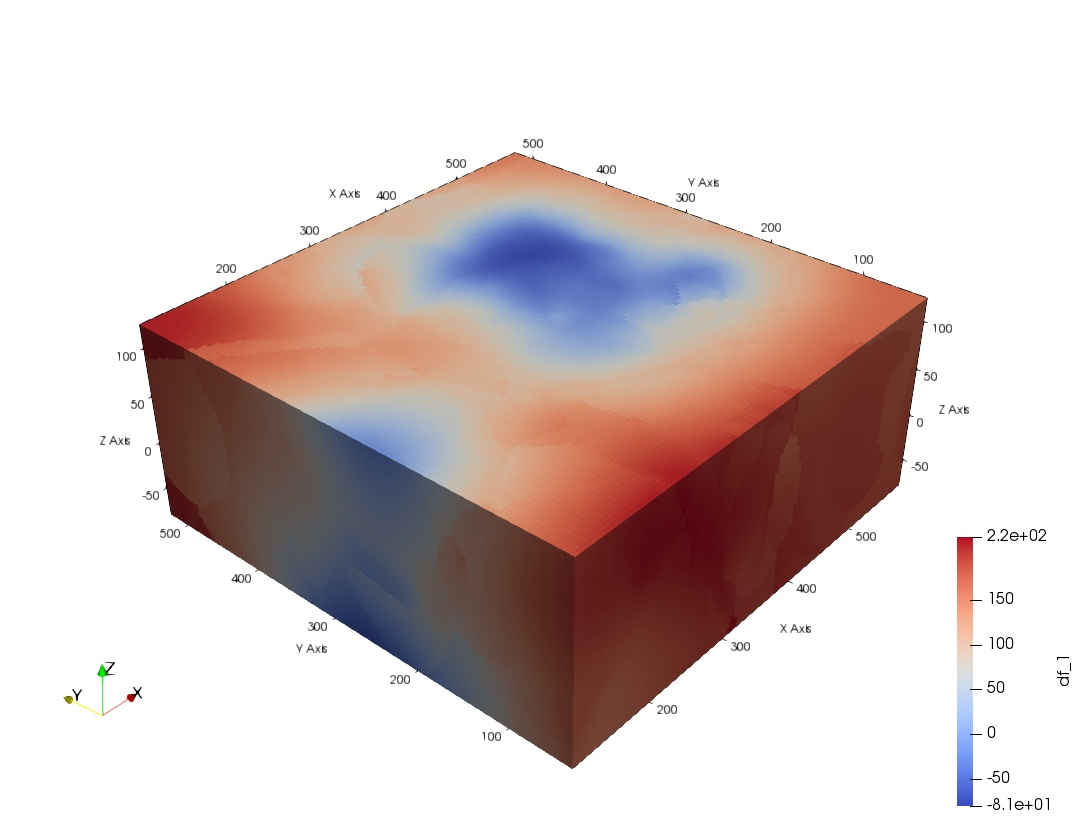
\includegraphics[width=.3\textwidth]{capitulo_2/kt3d100.jpeg}\label{<figure2>}}
		\subfloat[][RBF global]{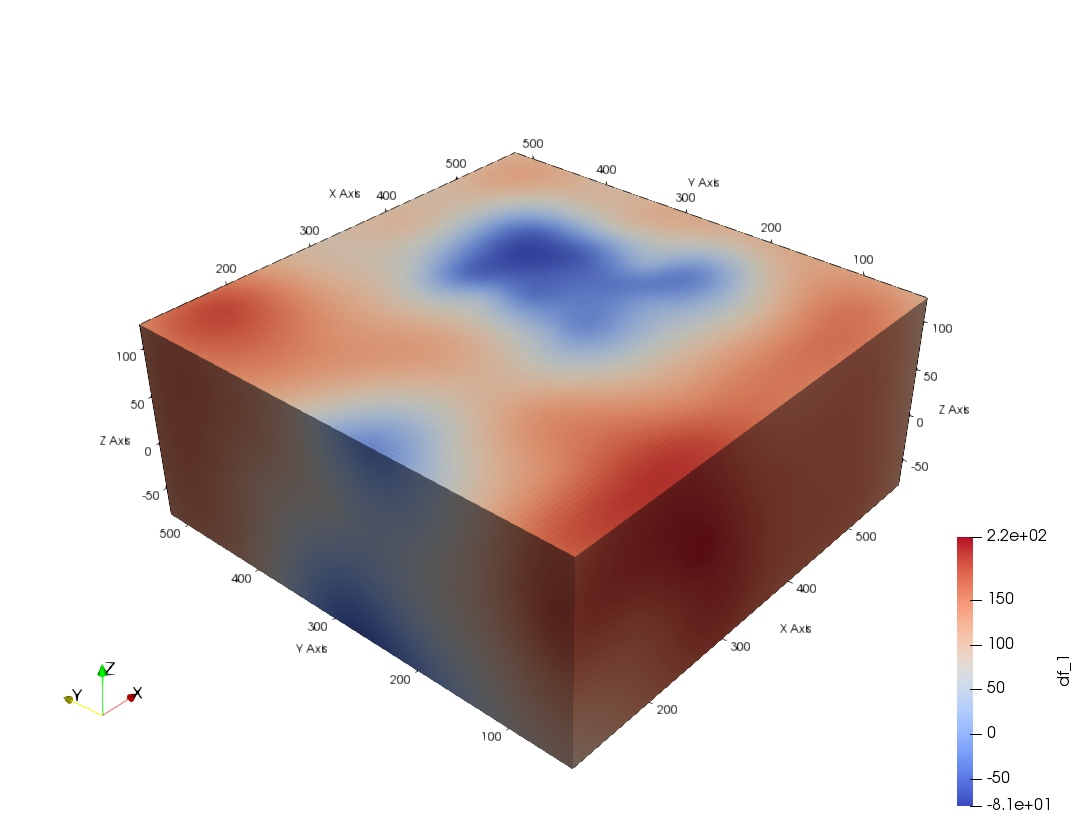
\includegraphics[width=.3\textwidth]{capitulo_2/rbf.jpeg}\label{<figure2>}}
	\end{figure}
\end{frame}

\begin{frame}{Decomposição do domínio}

Transforma um problema volumoso e que demanda muito esforço computacional em diversos problemas menores e eficientes que são, ao final, unidos.

\begin{figure}[H]
	\caption{\label{pou}Esquema mostrando o particionamento.}
	\begin{center}
		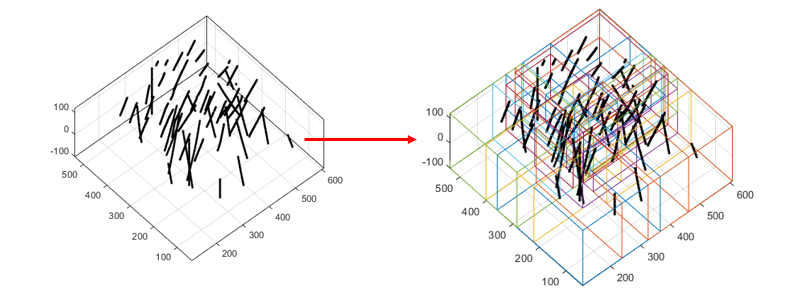
\includegraphics[width=0.9\textwidth]{capitulo_2/pou.jpg}
	\end{center}
	%\legend{Fonte: \citeonline{martin_boisvert_review_rbf}}
\end{figure}
\end{frame}

\begin{frame}{Benchmark}

Todos os algoritmos utilizados são da biblioteca GSLib e foram executados em um core i7 7700HQ @ 2.8 GHz com 16 Gb de RAM.

\begin{table}[H]
	\centering
	\resizebox{\textwidth}{!}{%
		\begin{tabular}{lllll}
			Método & Tempo grid grosso & Tempo grid fino & Classificação errônea grosso & Classificação errônea fino \\ \hline
			krigagem global isotrópica & 28min &  & 121 &  \\
			krigagem global anisotrópica & 30min 34s &  & 282 &  \\
			krigagem ordinária anisotrópica (40) & 1min 3s & 38min & 137 & 135 \\
			krigagem ordinária anisotrópica (100) &  & 45min 51s &  & 181 \\
			RBF isotrópico & 21.5s &  & 57 &  \\
			RBF anisotrópico &  & 1min 22s &  & 38 \\
			Particionado RBF anisotrópico &  & 1min 2s &  & 39 \\
			Particionado RBF artefatos & 16.5s &  &  & 29 \\
			LVA OK &  &  & 8 &  \\
			LVA RBF &  &  &  & 8 \\
			Krigagem dos indicadores &  & 33min 27s &  & 2 \\ \hline
		\end{tabular}%
	}
	\caption{\textit{Benchmark} dos diferentes métodos de interpolação.} \label{bench}
\end{table}
\end{frame}

\subsection{Visualização do modelo geológico}

\begin{frame}{Visualização do modelo geológico}

Um bom palpite inicial para a interface que separa os domínios no espaço, seria a linha (em duas dimensões) ou superfície (em três dimensões) que corresponda ao valor zero da função distância assinalada

\begin{figure}[H]
	\caption{Iso superfícies para a categoria 1 extraída dos diferentes modelos implícitos.} \label{isosup}
	\centering
	\subfloat[][OK com 40 amostras]{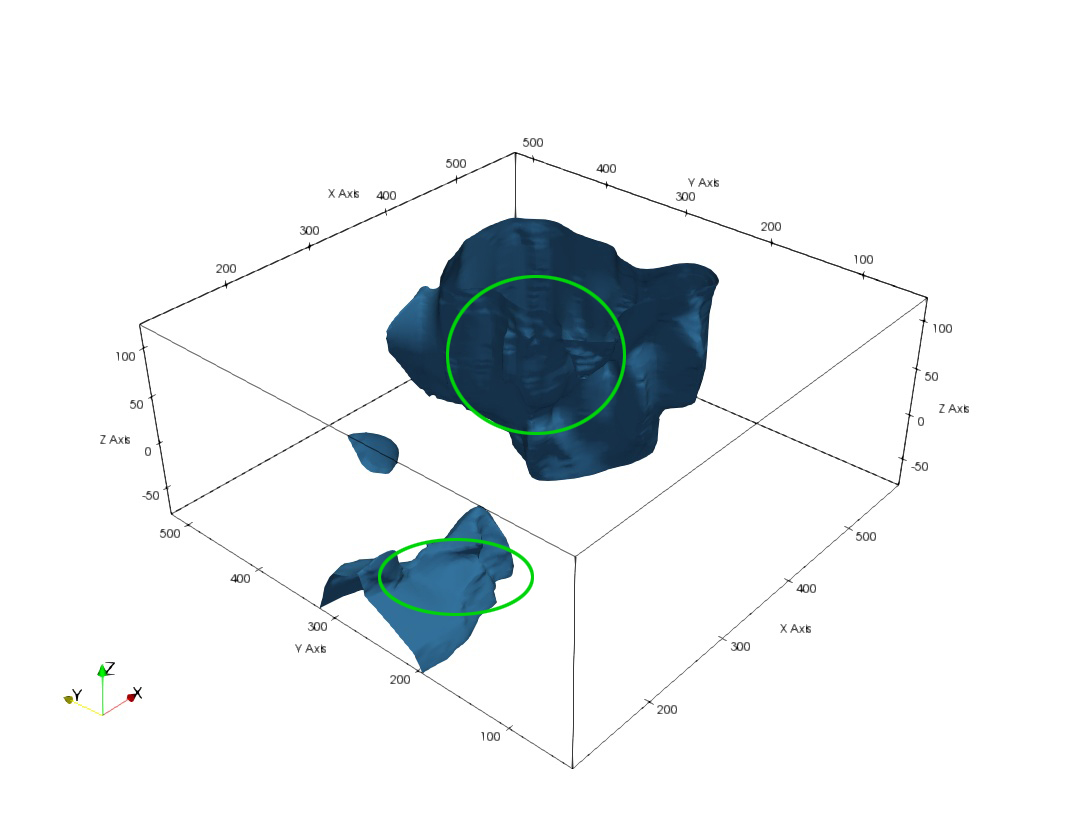
\includegraphics[width=.3\textwidth]{capitulo_2/isokt3d40.jpeg}\label{<figure1>}}
	\subfloat[][OK com 100 amostras]{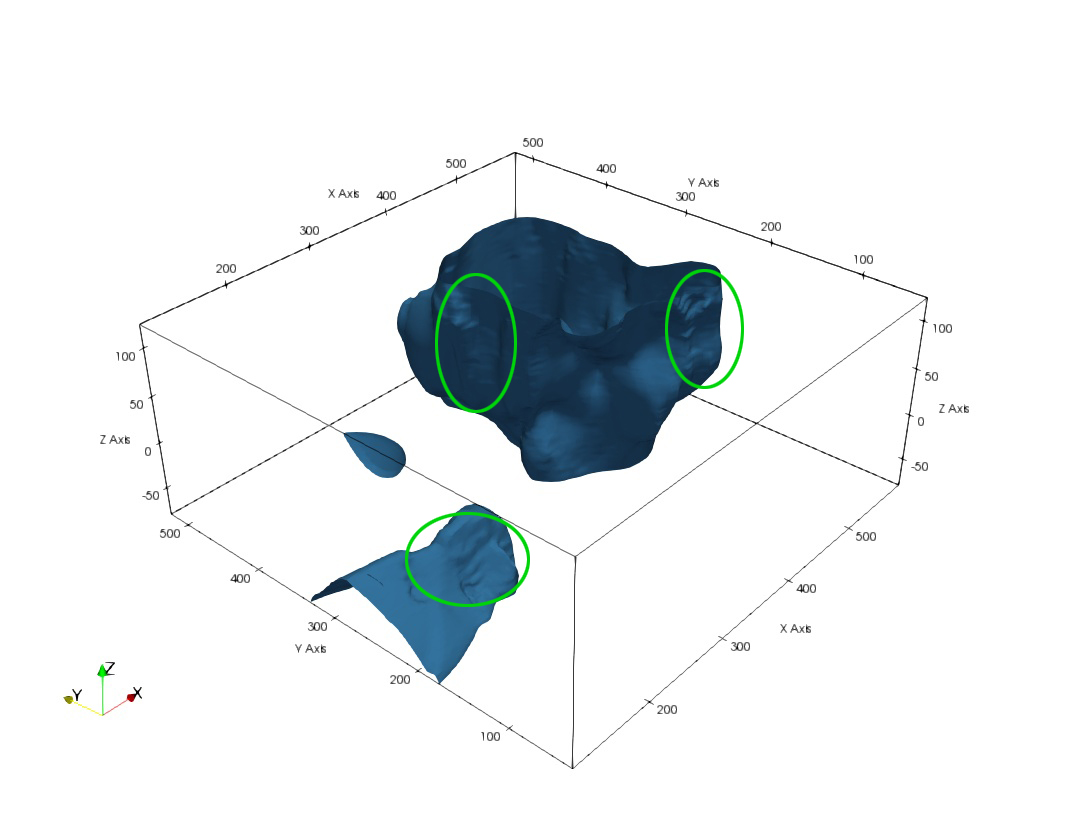
\includegraphics[width=.3\textwidth]{capitulo_2/isokt3dn100.jpeg}\label{<figure2>}}
	\subfloat[][RBF global]{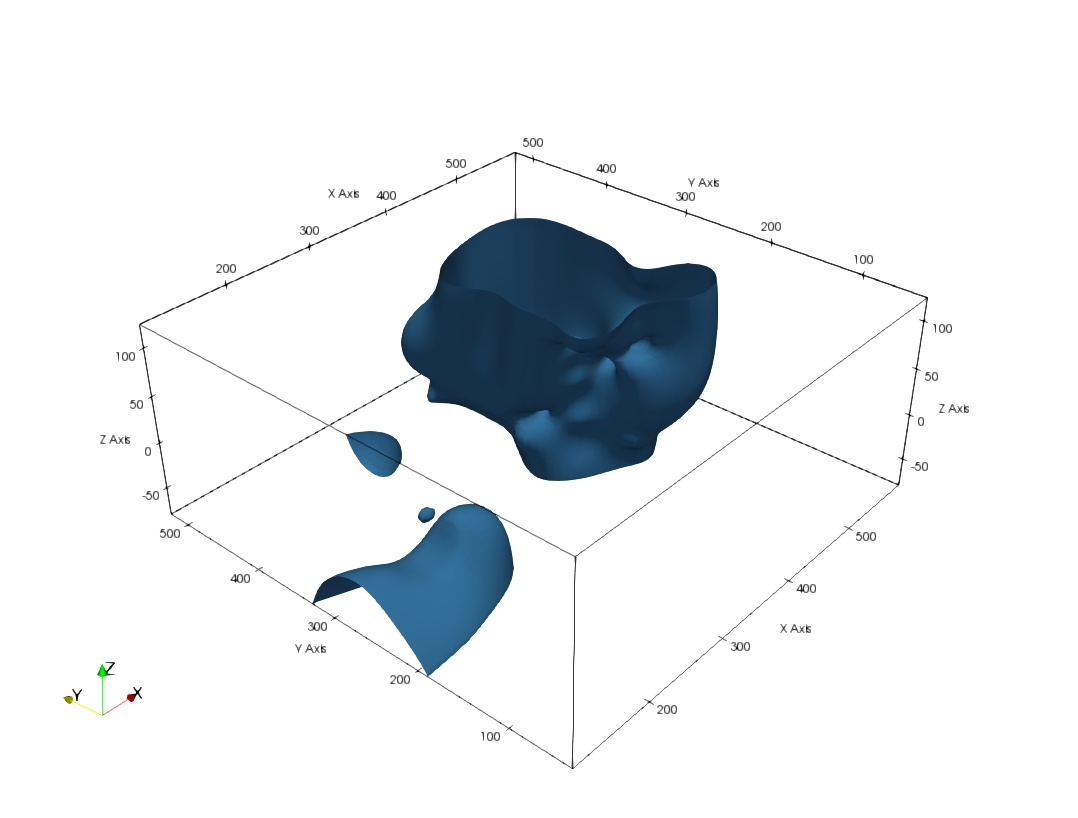
\includegraphics[width=.3\textwidth]{capitulo_2/isorbf.jpeg}\label{<figure2>}}
\end{figure}
\end{frame}

\begin{frame}{Visualização do modelo geológico}
	\begin{figure}[H]
		\caption{Iso superfície extraída do modelo implícito interpolado por RBF para a categoria 1.} \label{iso_cat1}
		\centering
		\subfloat[][Vista 1]{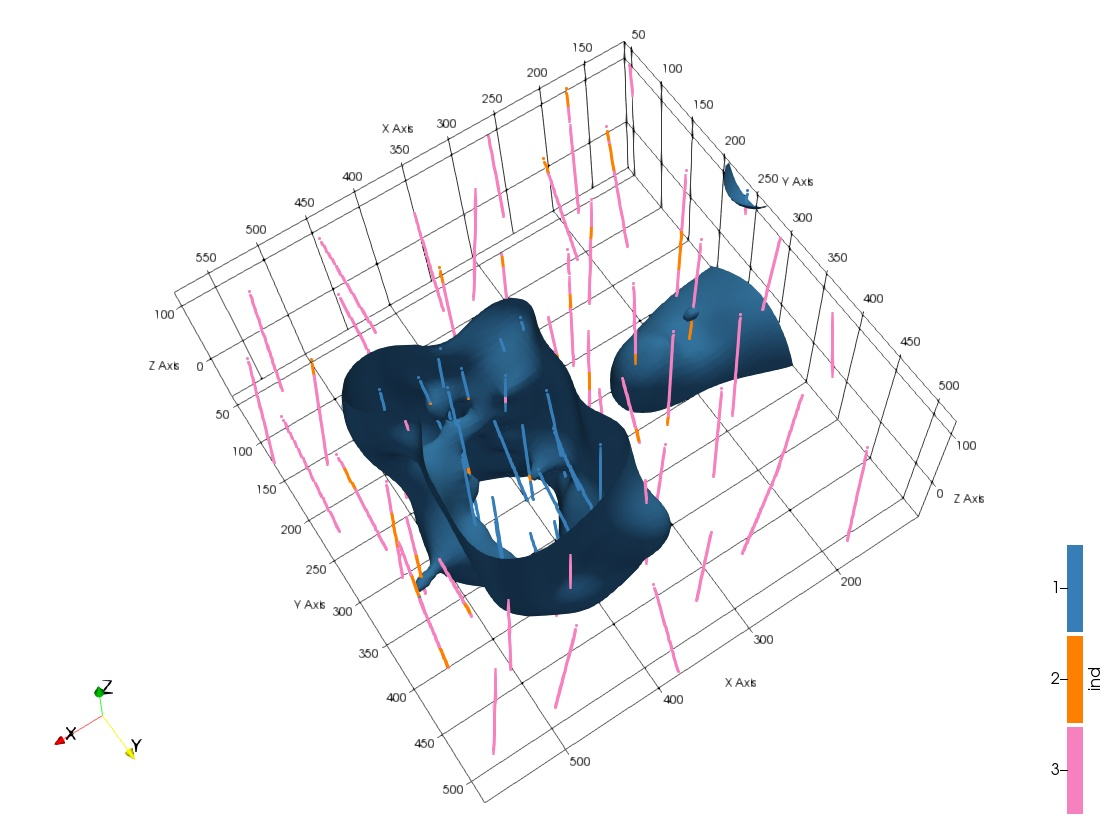
\includegraphics[width=.5\textwidth]{capitulo_2/iso_cat1_rbf.jpeg}\label{<figure1>}}
		\subfloat[][Vista 2]{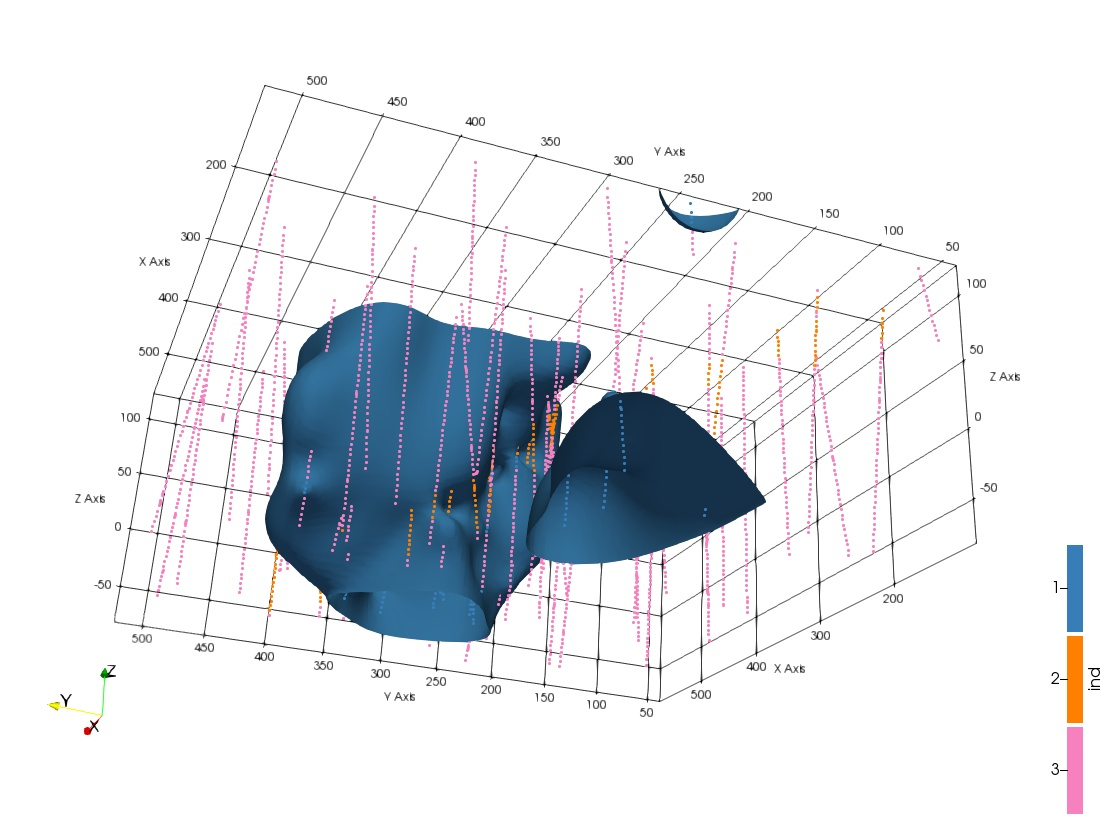
\includegraphics[width=.5\textwidth]{capitulo_2/iso_cat1_rbf2.jpeg}\label{<figure2>}}
	\end{figure}
\end{frame}

\begin{frame}{Visualização do modelo geológico}
\begin{figure}[H] 
	\caption{Iso superfície extraída do modelo implícito interpolado por RBF para a categoria 2.} \label{iso_cat2}
	\centering
	\subfloat[][Vista 1]{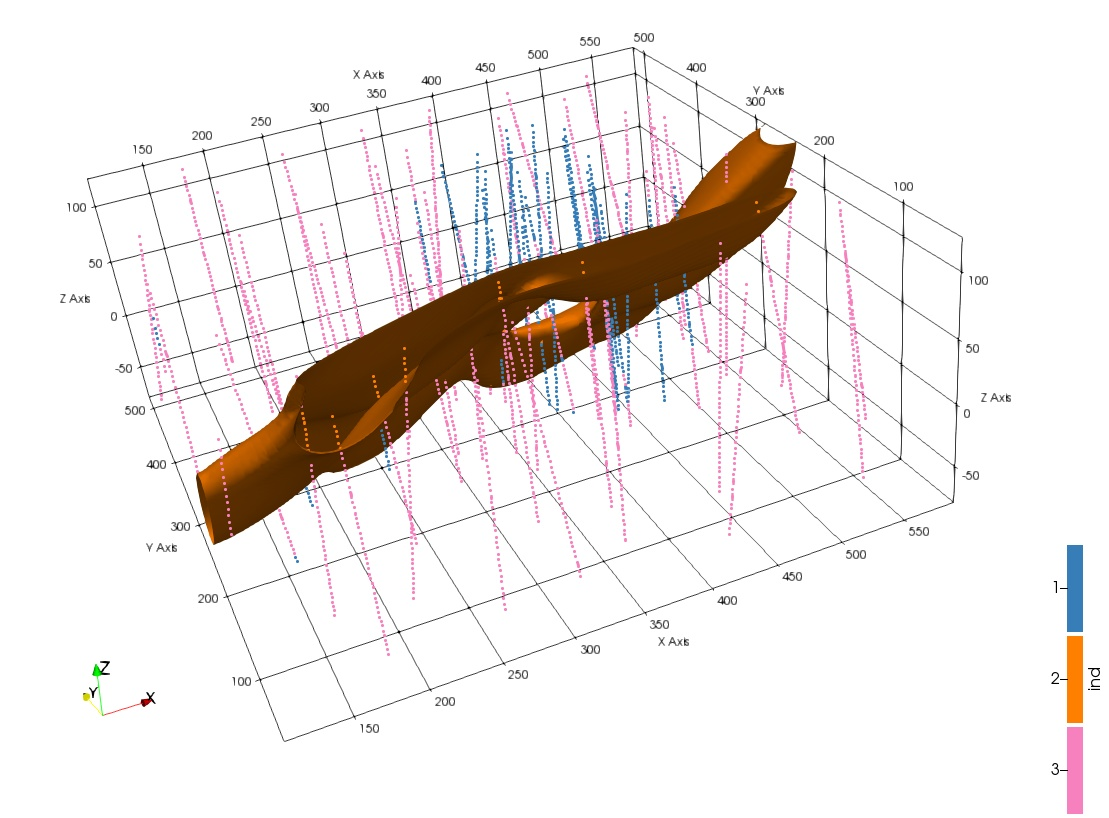
\includegraphics[width=.5\textwidth]{capitulo_2/iso_cat2_rbf.jpeg}\label{<figure1>}}
	\subfloat[][Vista 2]{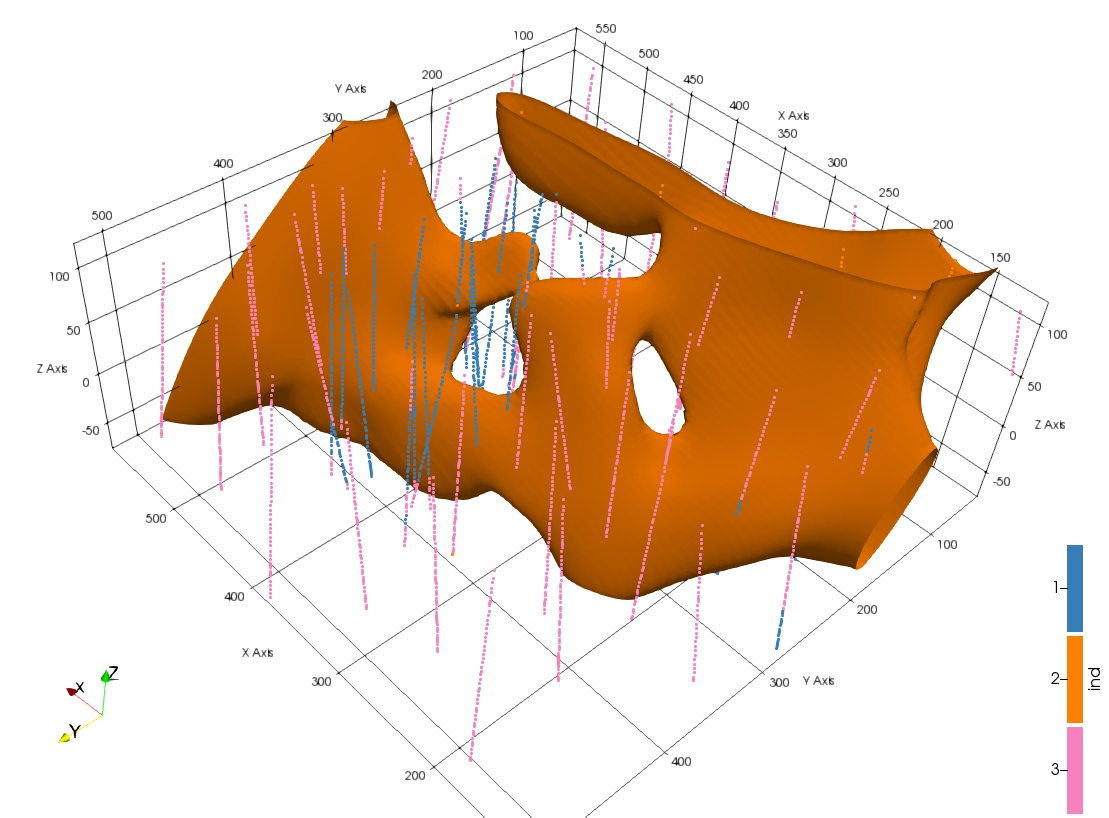
\includegraphics[width=.5\textwidth]{capitulo_2/iso_cat2_rbr2.jpeg}\label{<figure2>}}
\end{figure}
\end{frame}

\subsection{Adaptação para múltiplas categorias simultaneamente}

\begin{frame}{Adaptação para múltiplas categorias simultaneamente}

\begin{equation}
i_k(u_\alpha)=\begin{cases}
1,\:\textrm{se}\:z(u_\alpha)=k\\
0,\:\textrm{se}\:z(u_\alpha)\:\textrm{caso contrário}\end{cases} k=1,...,K
\label{eq_mult_ind}
\end{equation}

\begin{equation}
d_k(u_\alpha)=\begin{cases}
-\parallel u_\alpha-u_\beta\parallel,\:\textrm{se}\:i_k(u_\alpha)=1\\
+\parallel u_\alpha-u_\beta\parallel,\:\textrm{se}\:i_k(u_\alpha)=0\end{cases} k=1,...,K
\label{eq_mult_sg}
\end{equation}

\begin{equation}
d_k^*(u)=\sum\limits_{\alpha=1}^n \lambda_\alpha(u)d_k(u_\alpha)\quad k=1,...,K
\label{eq_mult_ok}
\end{equation}

\begin{equation}
i^*(u)=k'\;\text{de modo que}\;d_{k'}^*=min\{d_k^*(u)\}_{k=1}^K
\label{eq_mult_rt}
\end{equation}

\end{frame}

\begin{frame}{Adaptação para múltiplas categorias simultaneamente}
\begin{figure}[H]
	\caption{\label{mult_cat}Esquema para criação de um modelo implícito multi categórico.}
	\begin{center}
		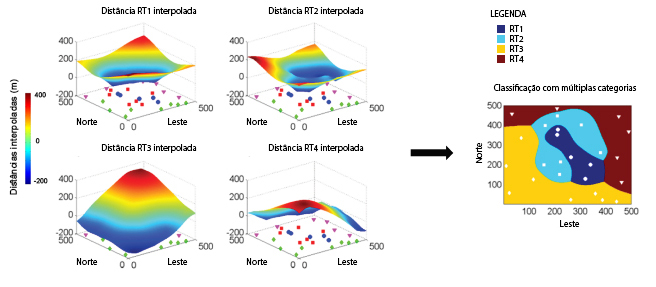
\includegraphics[width=\textwidth]{capitulo_2/mult_cat_legenda.jpg}
	\end{center}
	%\legend{Fonte: Modificado de \citeonline{silvageostatlessons}}
\end{figure}
\end{frame}

\begin{frame}{Adaptação para múltiplas categorias simultaneamente}
\begin{figure}[H]
	\caption{Modelo geológico multi categórico.} 
	\label{multi_cat_rbf}
	\centering
\subfloat[][Seções em XZ do modelo implícito gerado por RBF no \textit{grid} fino.]{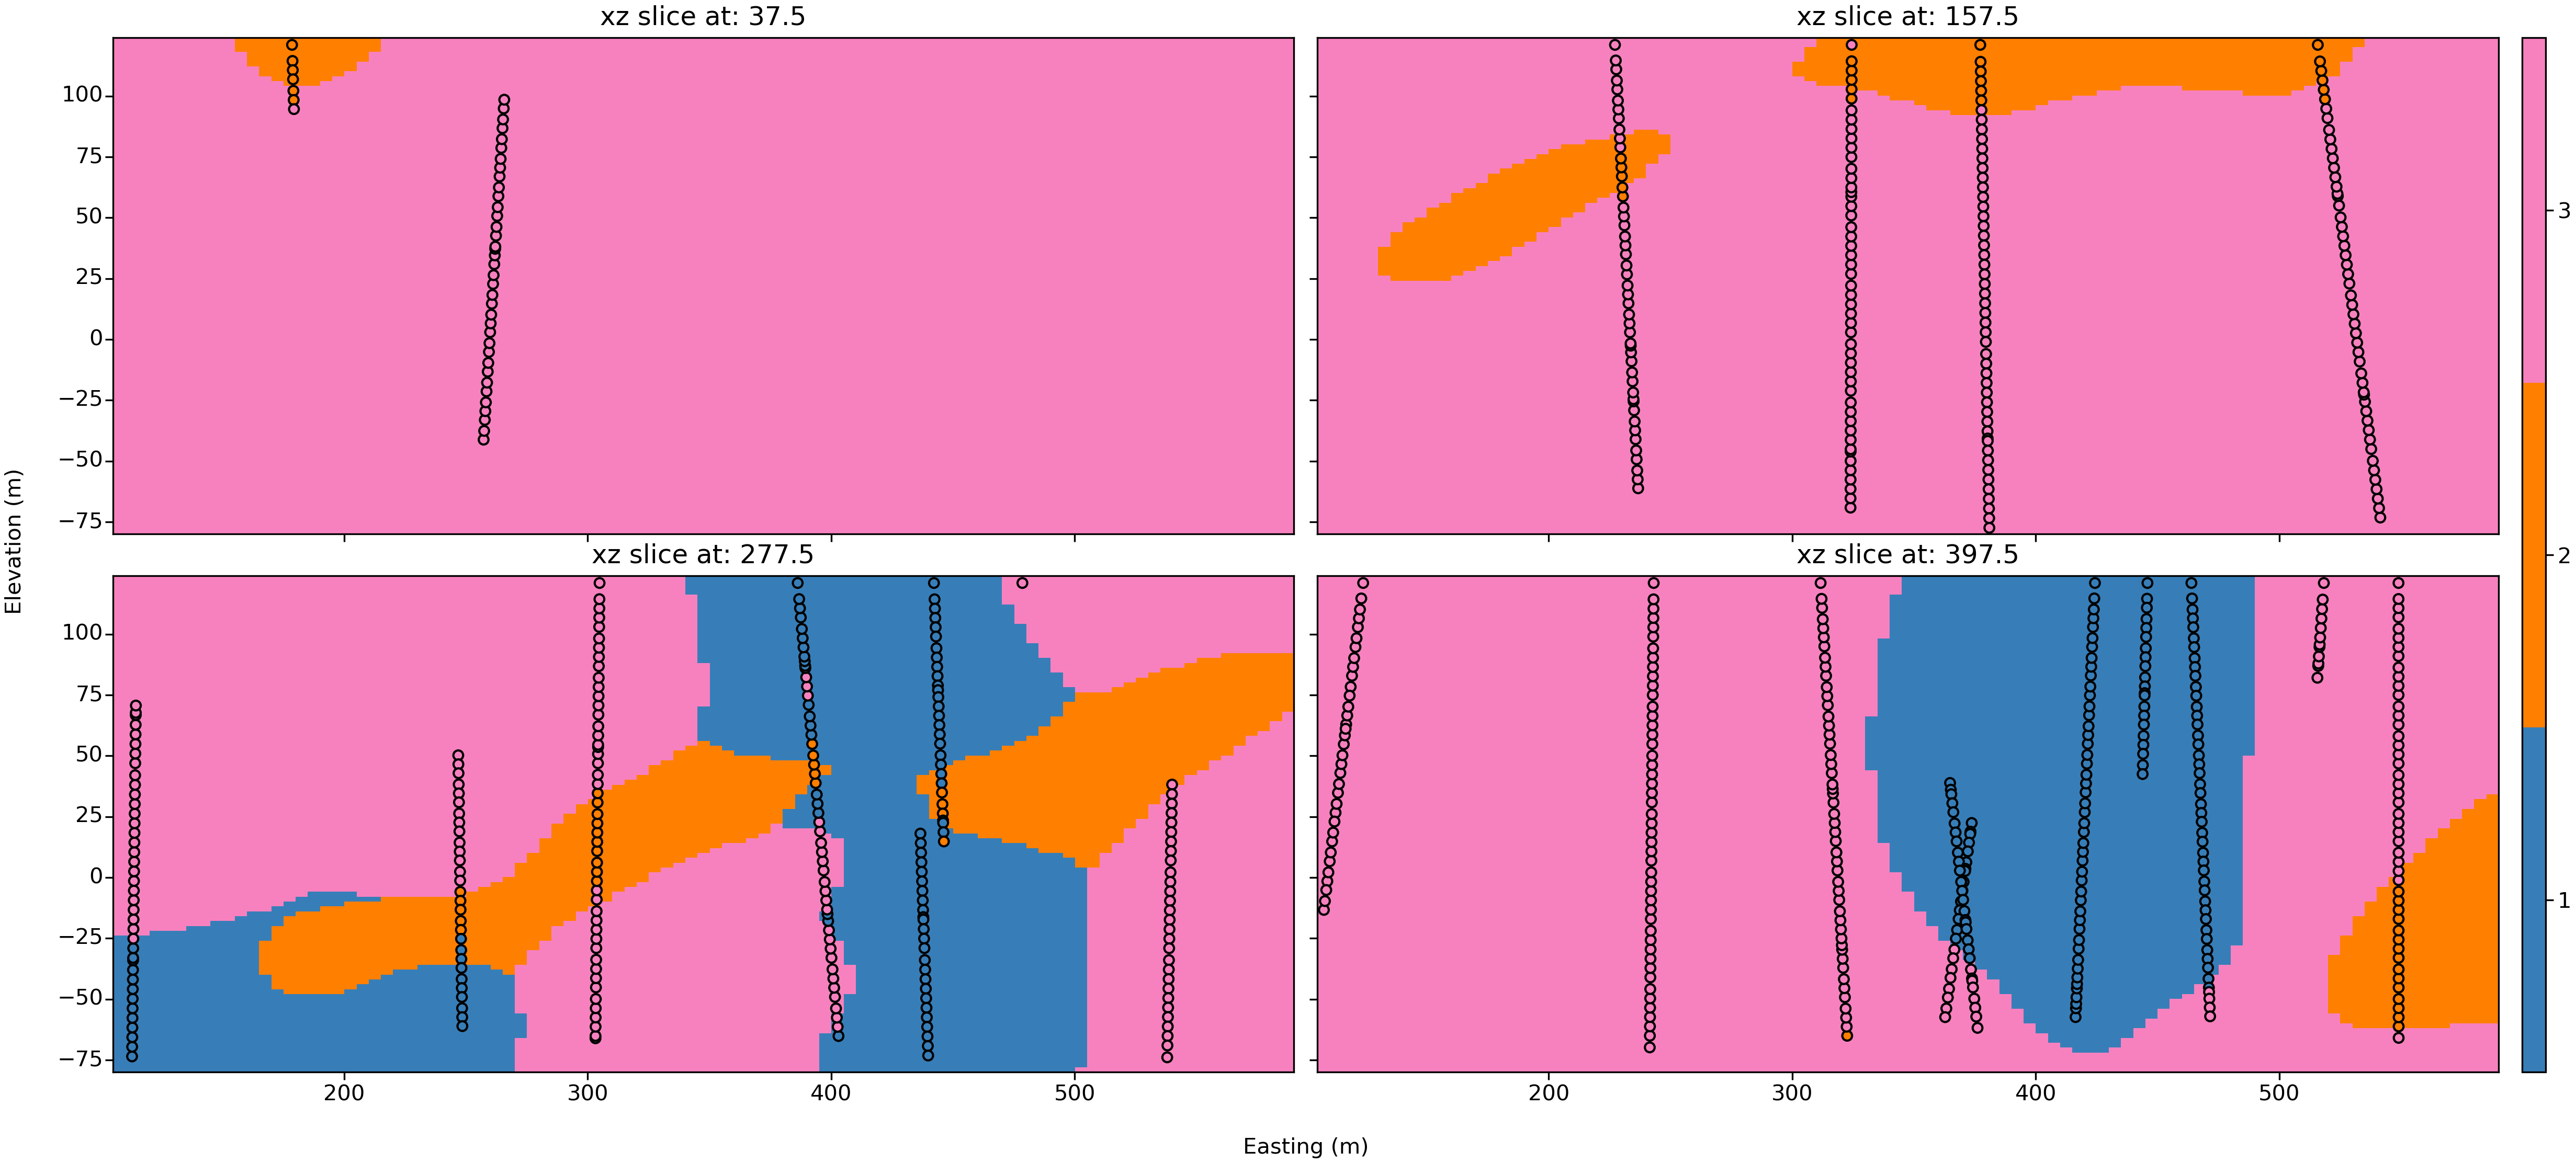
\includegraphics[width=.5\textwidth]{capitulo_2/anisofinexz.png}\label{<figure1>}}
\subfloat[][Seções em YZ do modelo implícito gerado por RBF no \textit{grid} fino.]{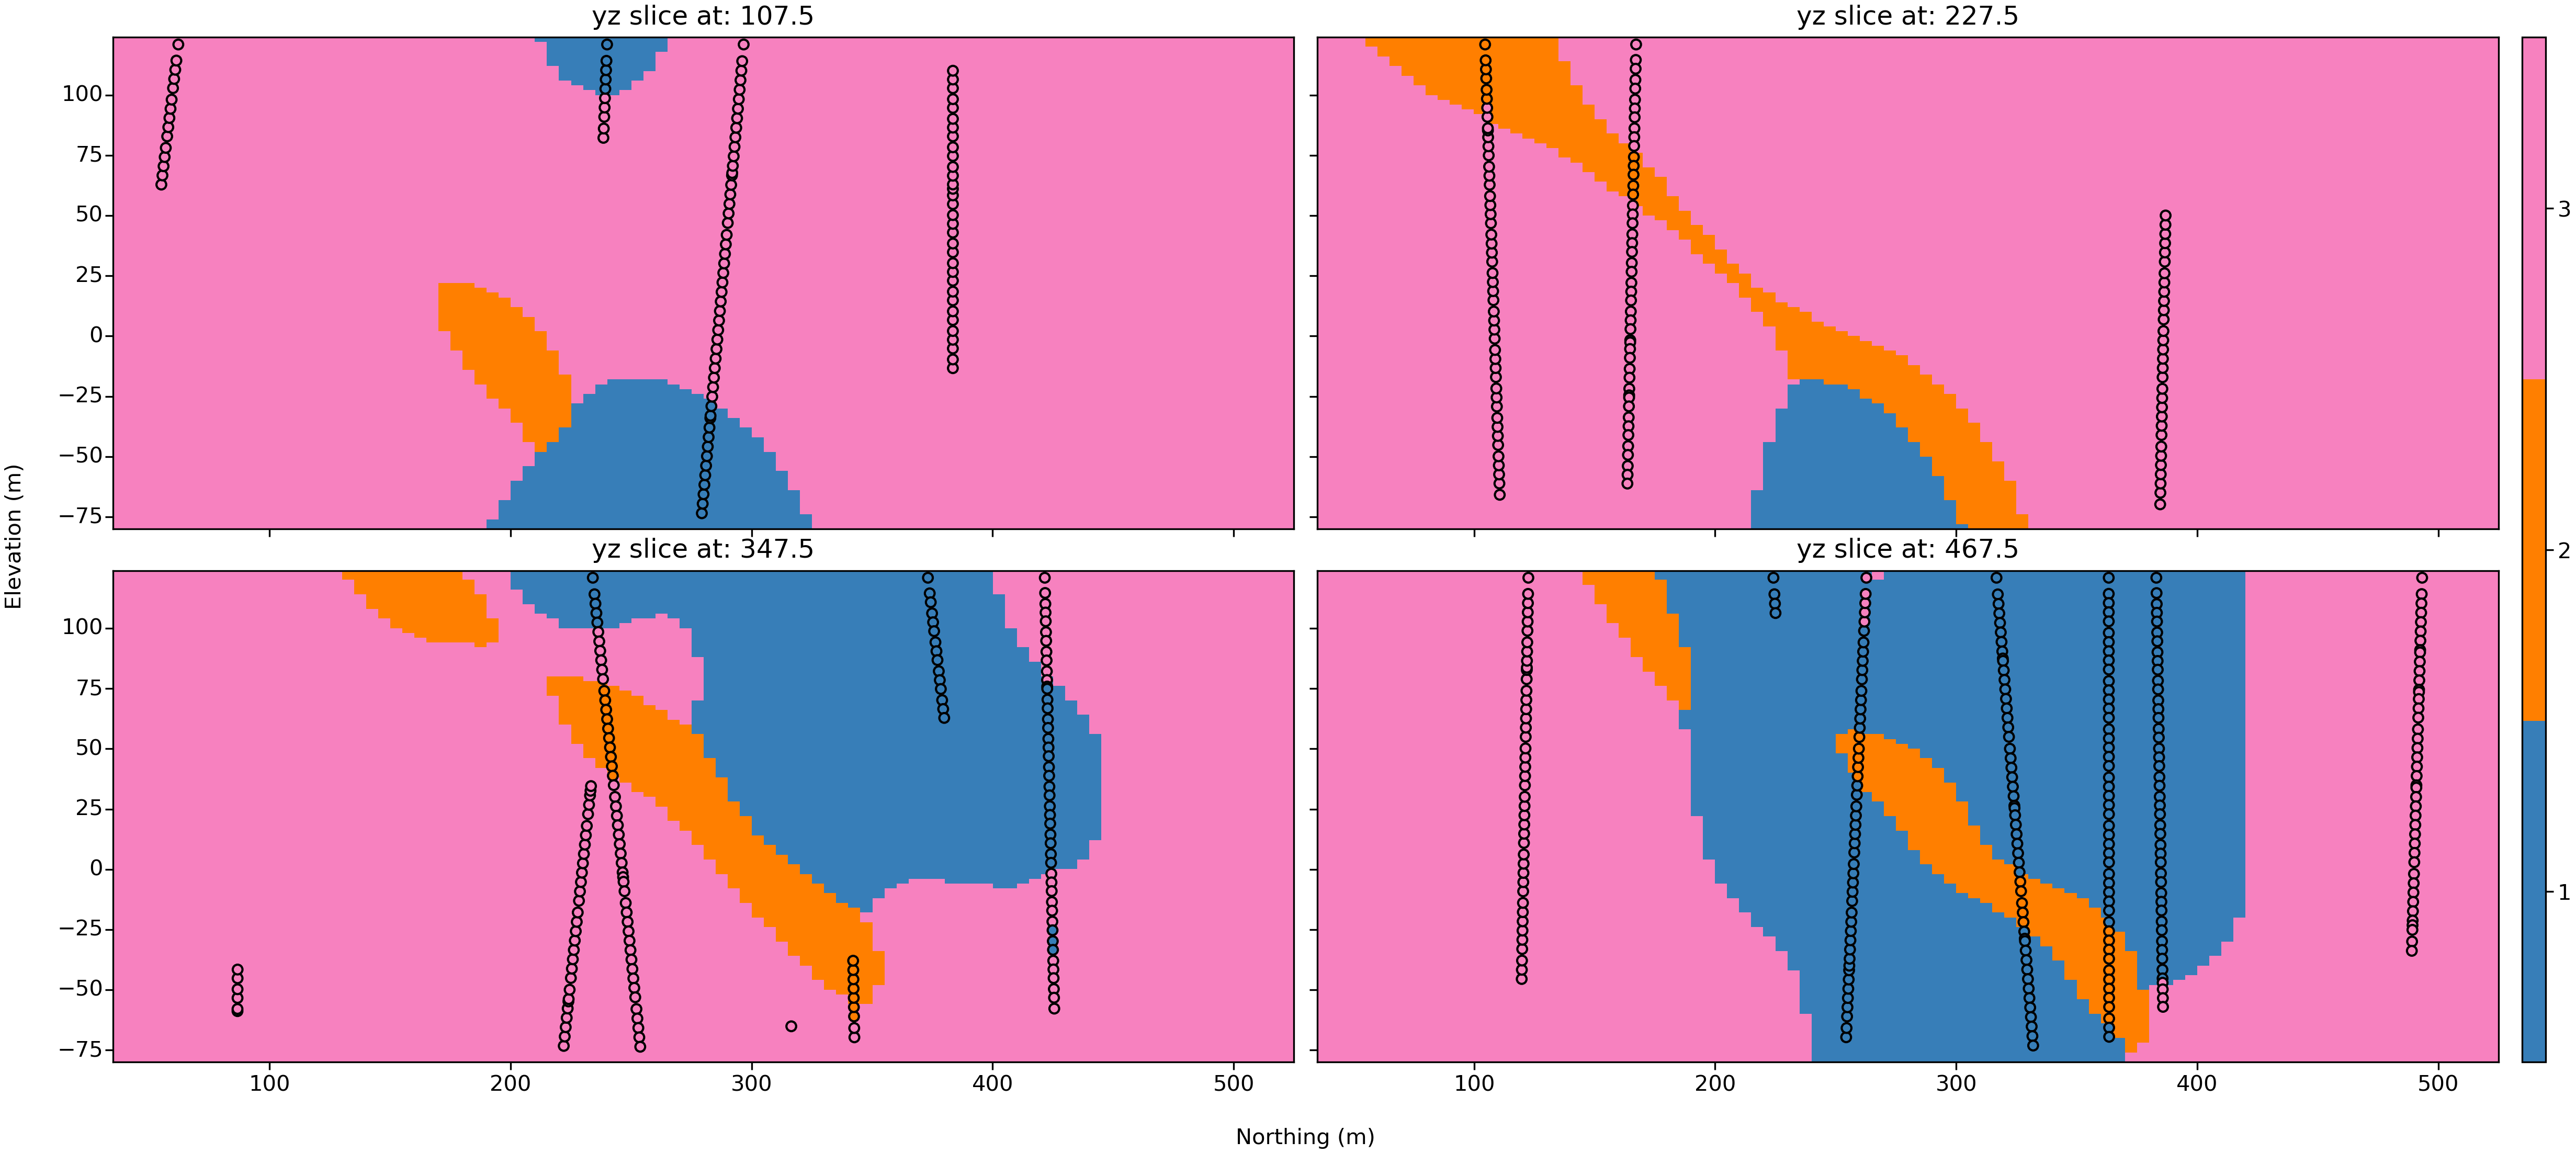
\includegraphics[width=.5\textwidth]{capitulo_2/anisofineryz.png}\label{<figure2>}}
\end{figure}

\end{frame}

\subsection{Incorporação da não estacionariedade de segunda ordem}

\begin{frame}{krigagem com anisotropia local variável}

\begin{figure}[H]
	\caption{\label{lva_krig_cartoon}Esquema mostrando os vetores de anisotropia local para cada nó do \textit{grid}.}
	\begin{center}
		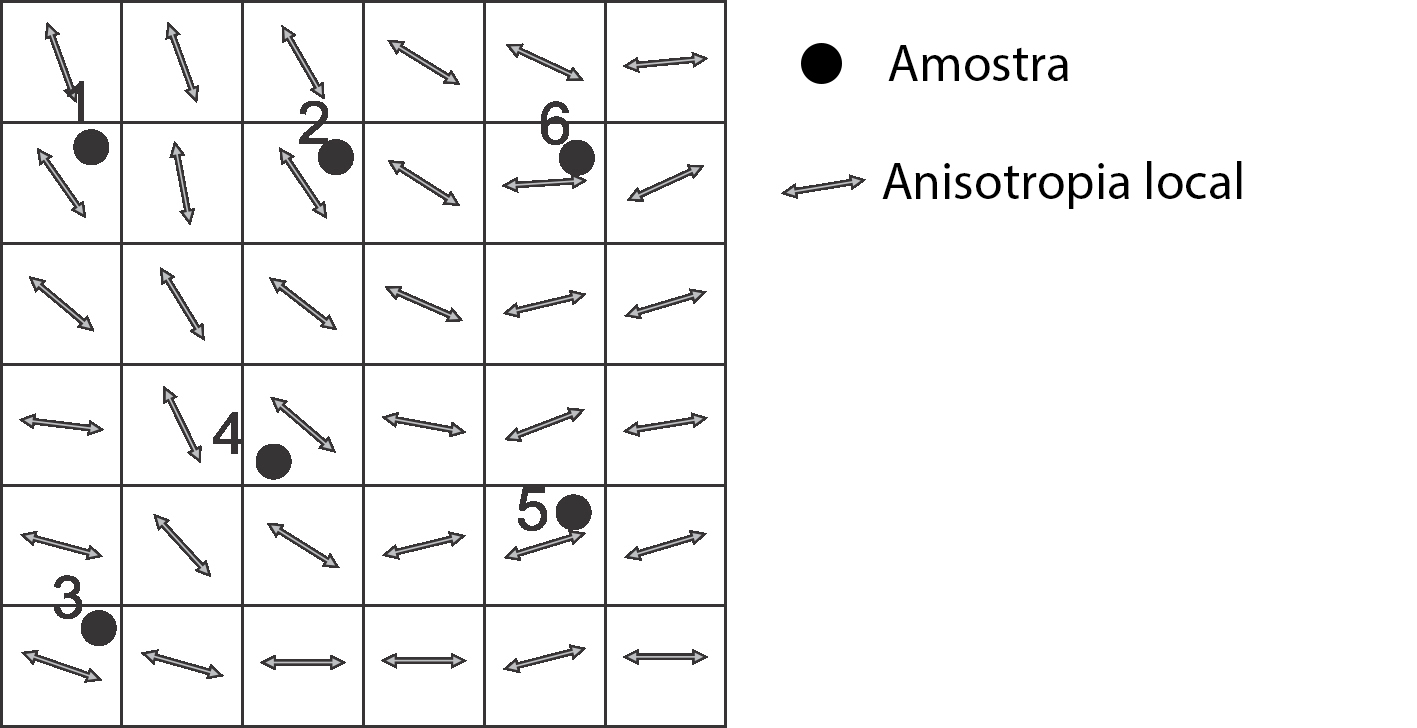
\includegraphics[width=0.8\textwidth]{capitulo_2/lvakrig1.jpg}
	\end{center}
	%\legend{Fonte: \citeonline{martin2017implicitmodeling}}
\end{figure}
	
\end{frame}

\begin{frame}
	\begin{figure}[H] 
		\caption{Iso superfície para a categoria 1 extraída de um modelo implícita gerado por krigagem com anisotropia local variável mostrando os vetores.} \label{lva_krig}
		\centering
		\subfloat[][Todos os vetores de anisotropia local]{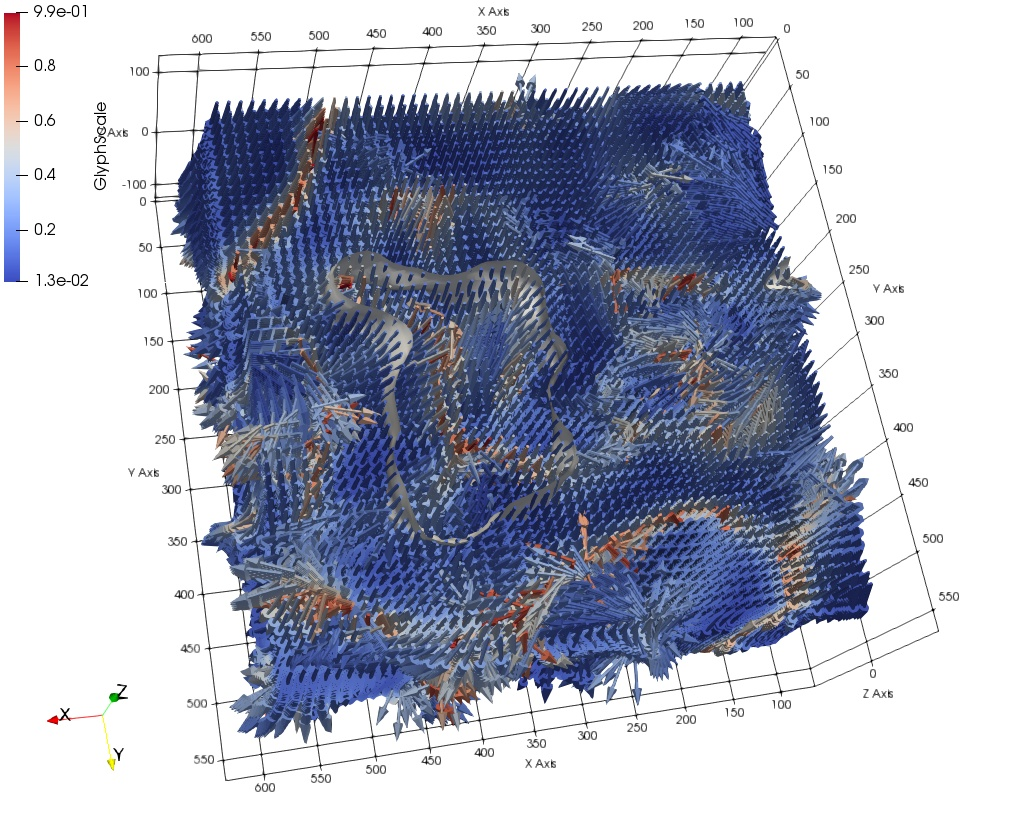
\includegraphics[width=.5\textwidth]{capitulo_2/lva_krig.jpeg}\label{<figure1>}}
		\subfloat[][Um vetor a cada 100.000 blocos]{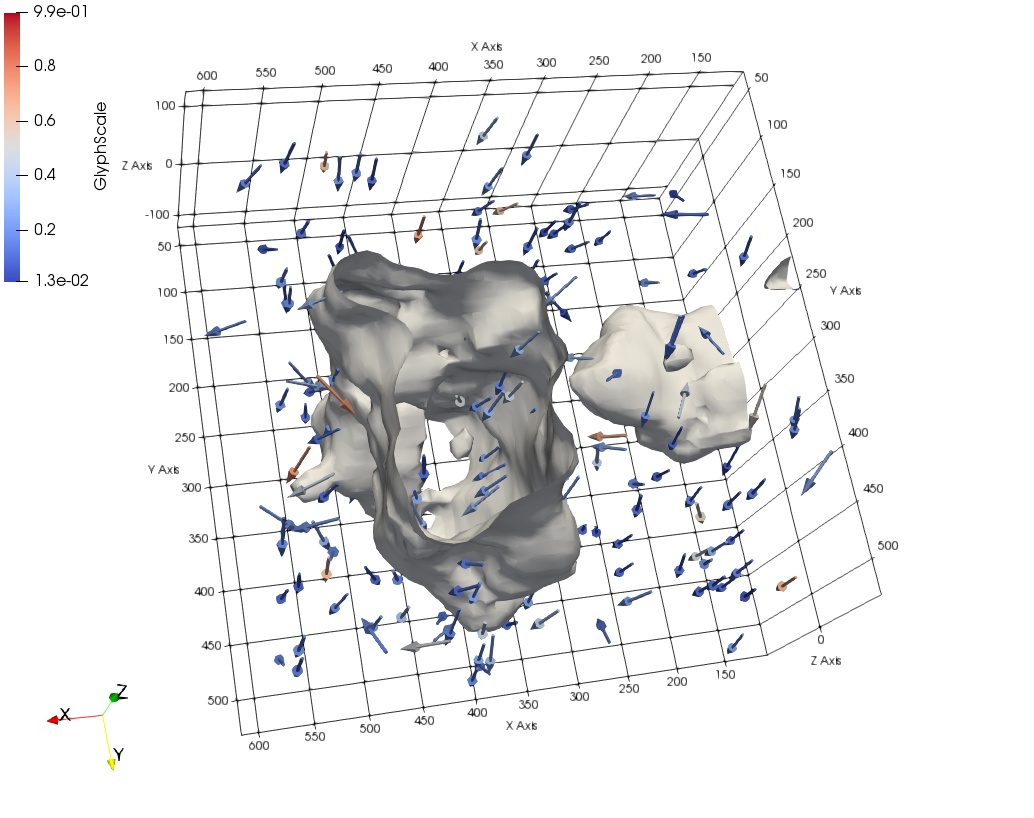
\includegraphics[width=.5\textwidth]{capitulo_2/lva_krig_100000.jpeg}\label{<figure2>}}
	\end{figure}
\end{frame}

\begin{frame}{Funções de bases radiais com anisotropia local variável}
	\begin{figure}[H]
		\caption{\label{lva_rbf+cartoon} Esquema mostrando os vetores de anisotropia local para cada centro de partição.}
		\begin{center}
			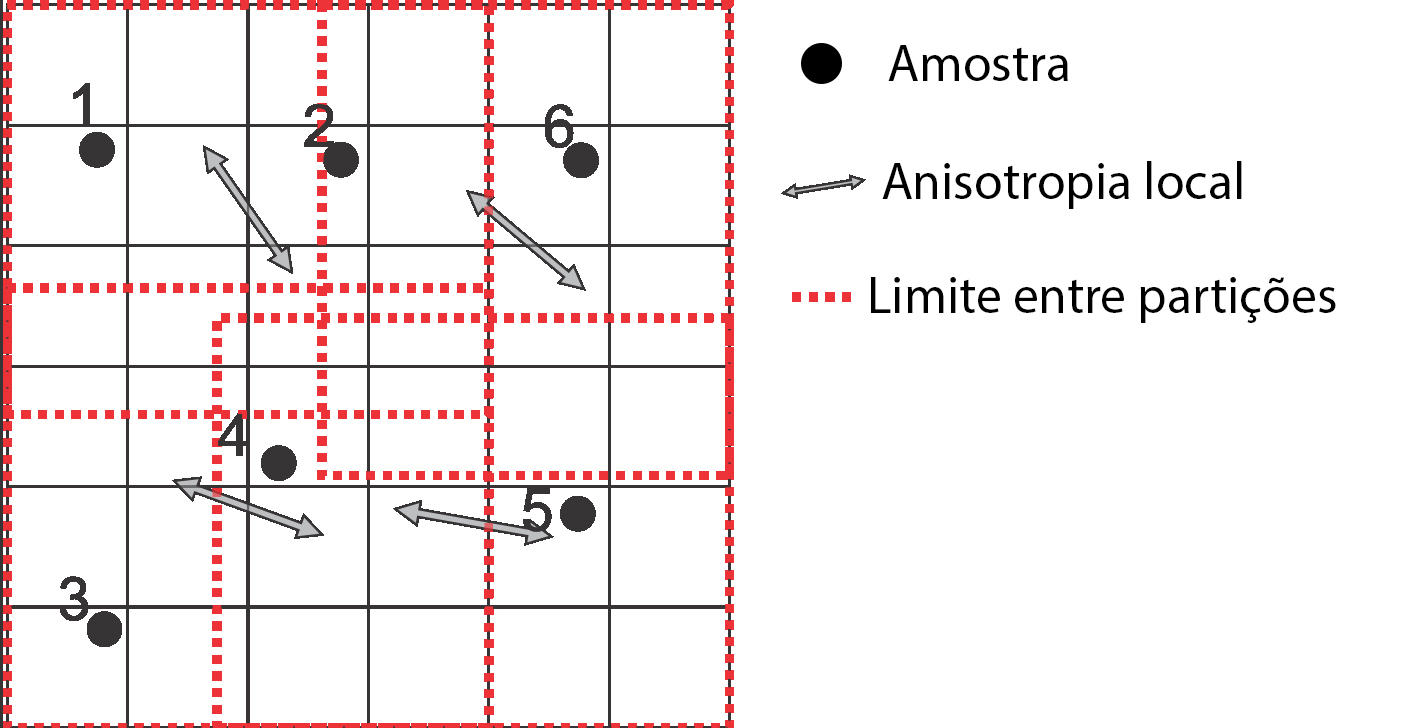
\includegraphics[width=0.8\textwidth]{capitulo_2/lvarbf1.jpg}
		\end{center}
		%\legend{Fonte: \citeonline{martin2017implicitmodeling}}
	\end{figure}
\end{frame}

\begin{frame}{Funções de bases radiais com anisotropia local variável}
	\begin{figure}[H]
		\caption{\label{rbf_iterref}Iso superfície para a categoria 1 extraída de um modelo implícita gerado por krigagem com anisotropia local variável mostrando os vetores.}
		\begin{center}
			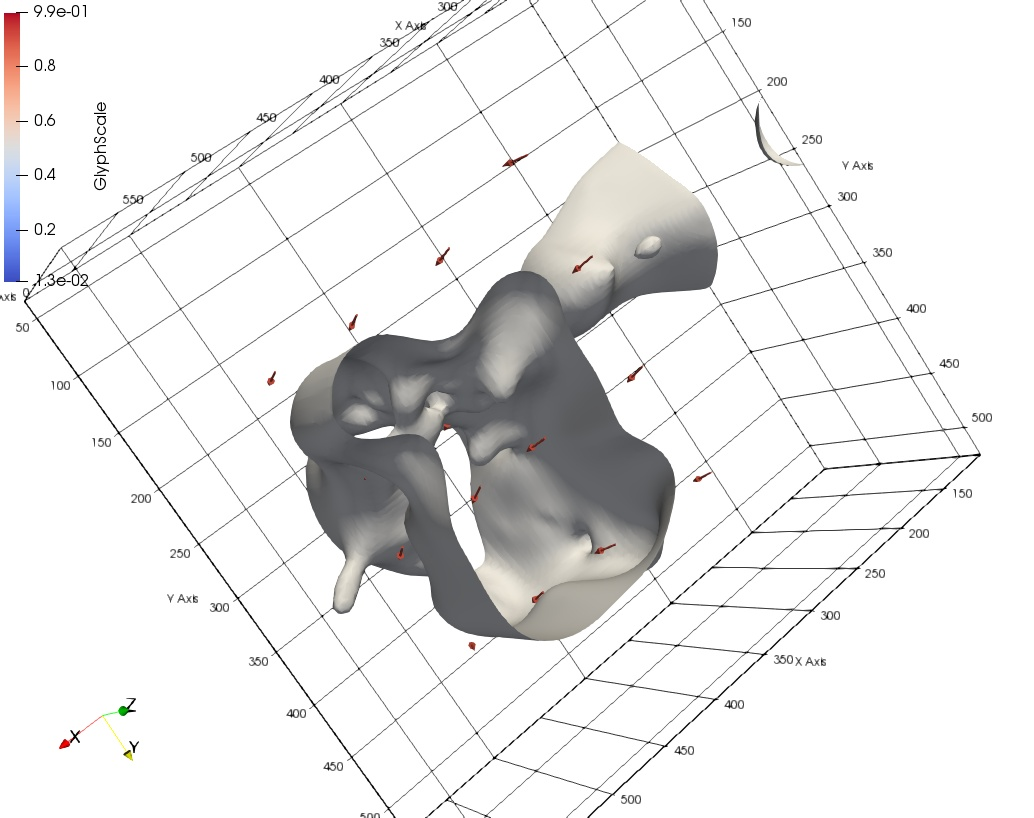
\includegraphics[width=0.5\textwidth]{capitulo_2/rbf_iterref.jpeg}
		\end{center}
		%\legend{Fonte: Modificado de \citeonline{silvageostatlessons}}
	\end{figure}
\end{frame}

\subsubsection{Refinamento iterativo}

\begin{frame}{Refinamento iterativo}

Extrair orientações locais de um modelo criado com anisotropia global e utilizar essas orientações em uma nova interpolação não estacionária resulta em um modelo geológico mais refinado considerando informação local.

	\begin{figure}[H]
		\caption{\label{iterref} Esquema mostrando etapas usando o refinamento iterativo para funções de bases radiais.}
		\begin{center}
			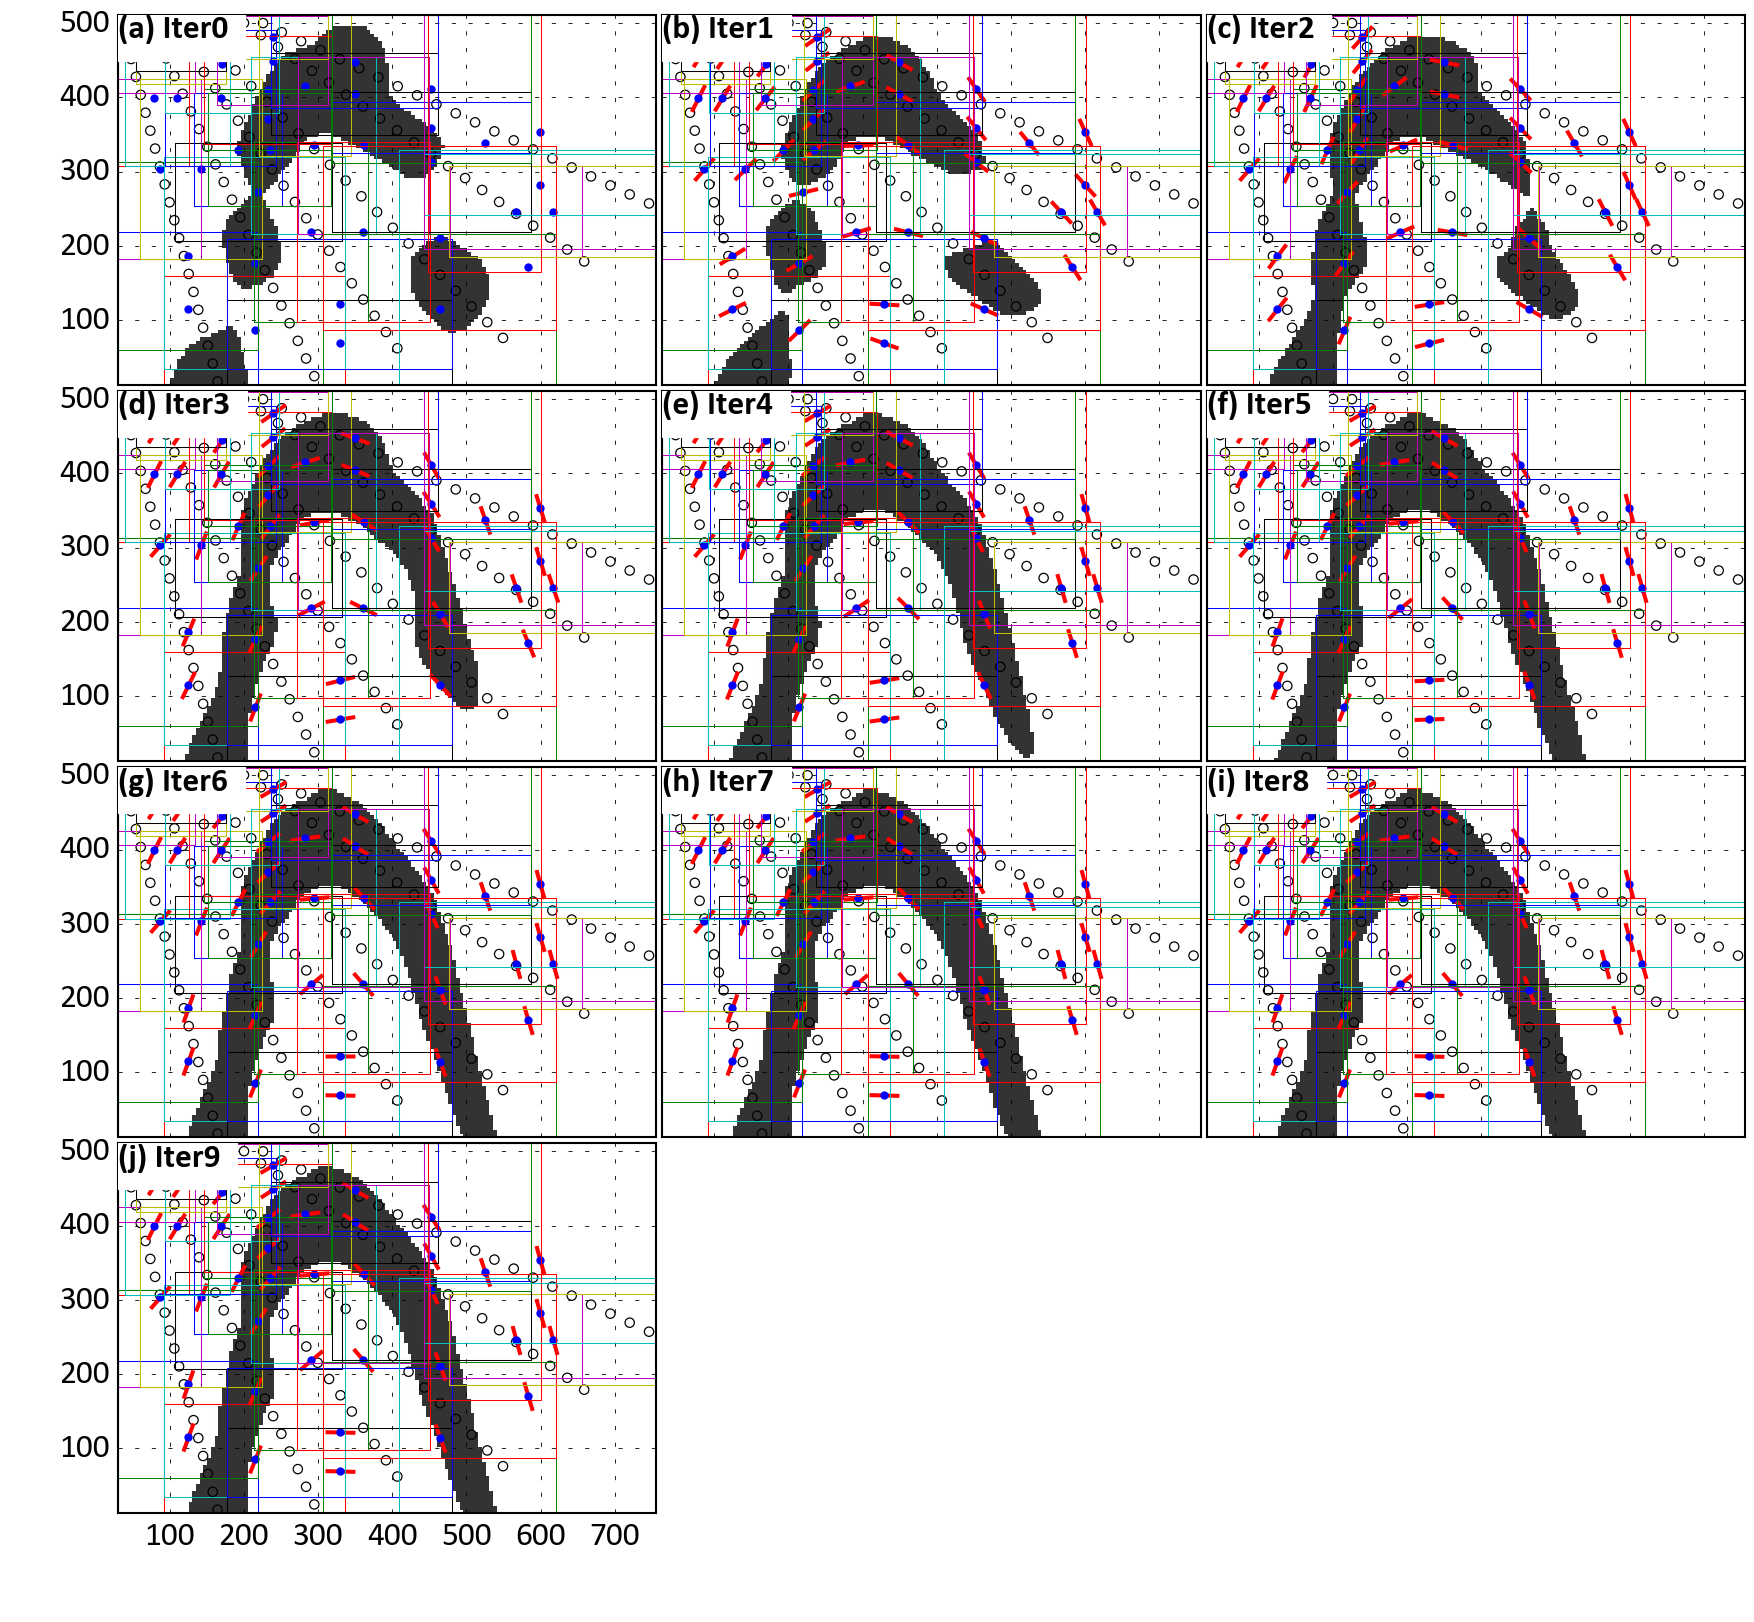
\includegraphics[width=0.3\textwidth]{capitulo_2/iterref.jpg}
		\end{center}
		%\legend{Fonte: \citeonline{martin2017implicitmodeling}}
	\end{figure}
\end{frame}

\subsection{Incorporação de informação secundária}

\begin{frame}{Incorporação de informação secundária}

\cite{manchuck_MLS} propõe o uso de uma regressão linear local chamada mínimos quadrados móveis (\textit{Moving least squares - MLS}) que ajusta uma função aos dados para integrar modelagem geológica implícita e explicita.

	\begin{figure}[H]
		\caption{Modelo geológico híbrido criado a partir de furos de sondagem e seções interpretadas.}\label{mls_model}
			\subfloat[][Seção mostrando furos e seções interpretadas.]{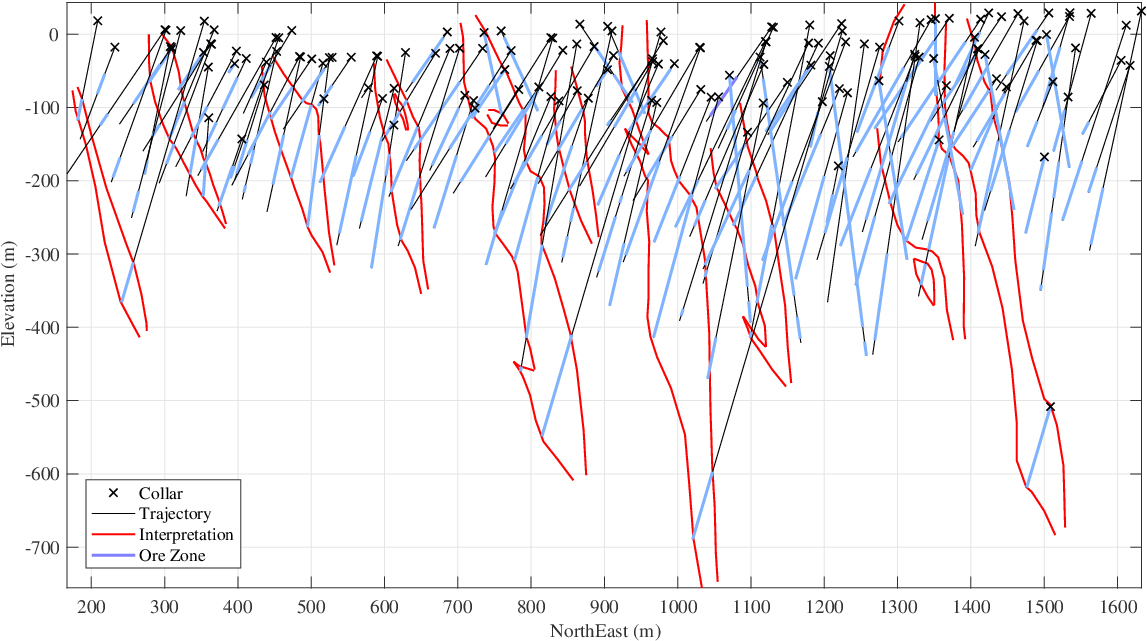
\includegraphics[width=0.3\textwidth]{capitulo_2/secoes.jpg}\label{a}}
			\subfloat[][Modelo implícito.]{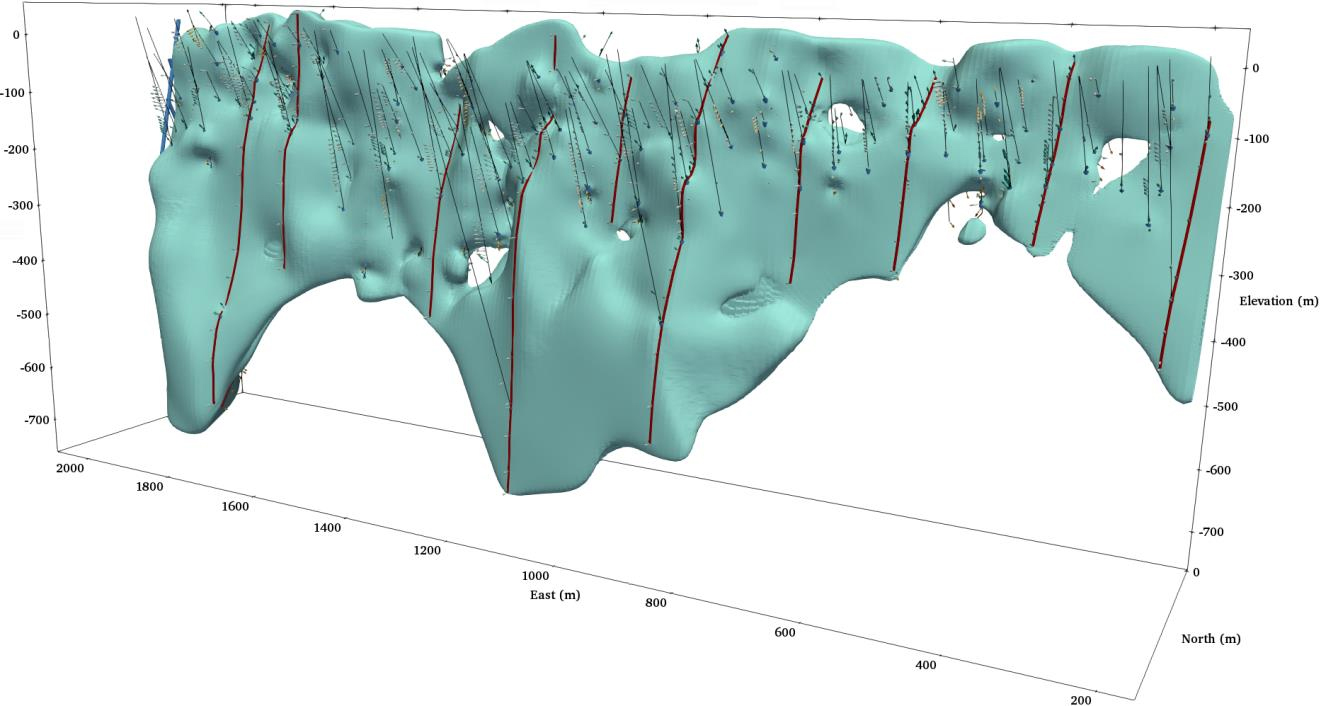
\includegraphics[width=0.3\textwidth]{capitulo_2/modelo_mls.jpg}\label{b}}
			%\legend{Fonte: \citeonline{manchuck_MLS}}
	\end{figure}
\end{frame}

\section{Avaliação da incerteza}

\subsection{Avaliação heurística da incerteza}

\begin{frame}{Avaliação heurística da incerteza}

Transformação das distâncias em probabilidades.
	\begin{equation}
	P(i(u)=k)=\frac{e^\frac{-d^*_k(u)}{\gamma}}{\sum_{k'=1}^{K}e^\frac{-d^*_k(u)}{\gamma}}
	\label{eq_softmax}
	\end{equation}
	
	\begin{figure}[H]
		\caption{\label{softmax_grafico}Distâncias estimadas em (a) e transformadas em probabilidades em (b) para um mesmo bloco, com cinco categorias.}
		\begin{center}
			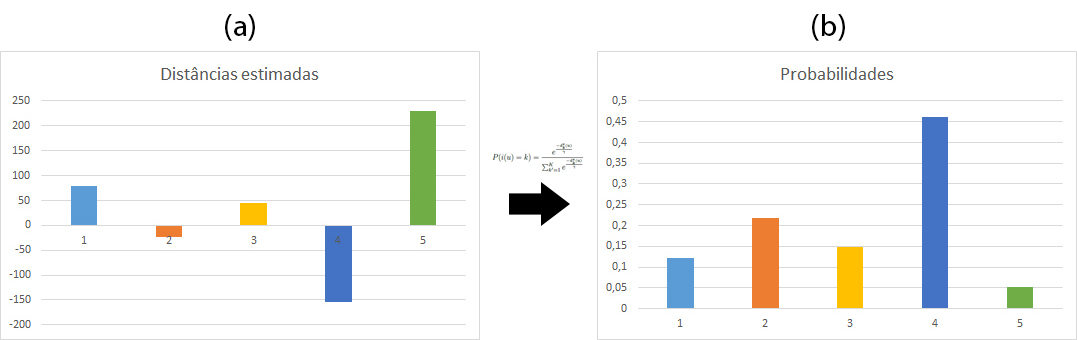
\includegraphics[width=0.7\textwidth]{capitulo_2/softmax_bars_final.jpg}
		\end{center}
		%\legend{Fonte: \citeonline{rolo_dissertacao}}
	\end{figure}
\end{frame}

\subsection{BOUNDSIM}

\begin{frame}{BOUNDSIM}

Krigagem simples com médias tomadas do histograma da média.

\begin{columns}
	\begin{column}{0.5\textwidth}
	\begin{figure}[H]
		\caption{\label{bs_df_1}Histograma do bootstrap espacial da média das distâncias assinaladas para a categoria 1.}
		\begin{center}
			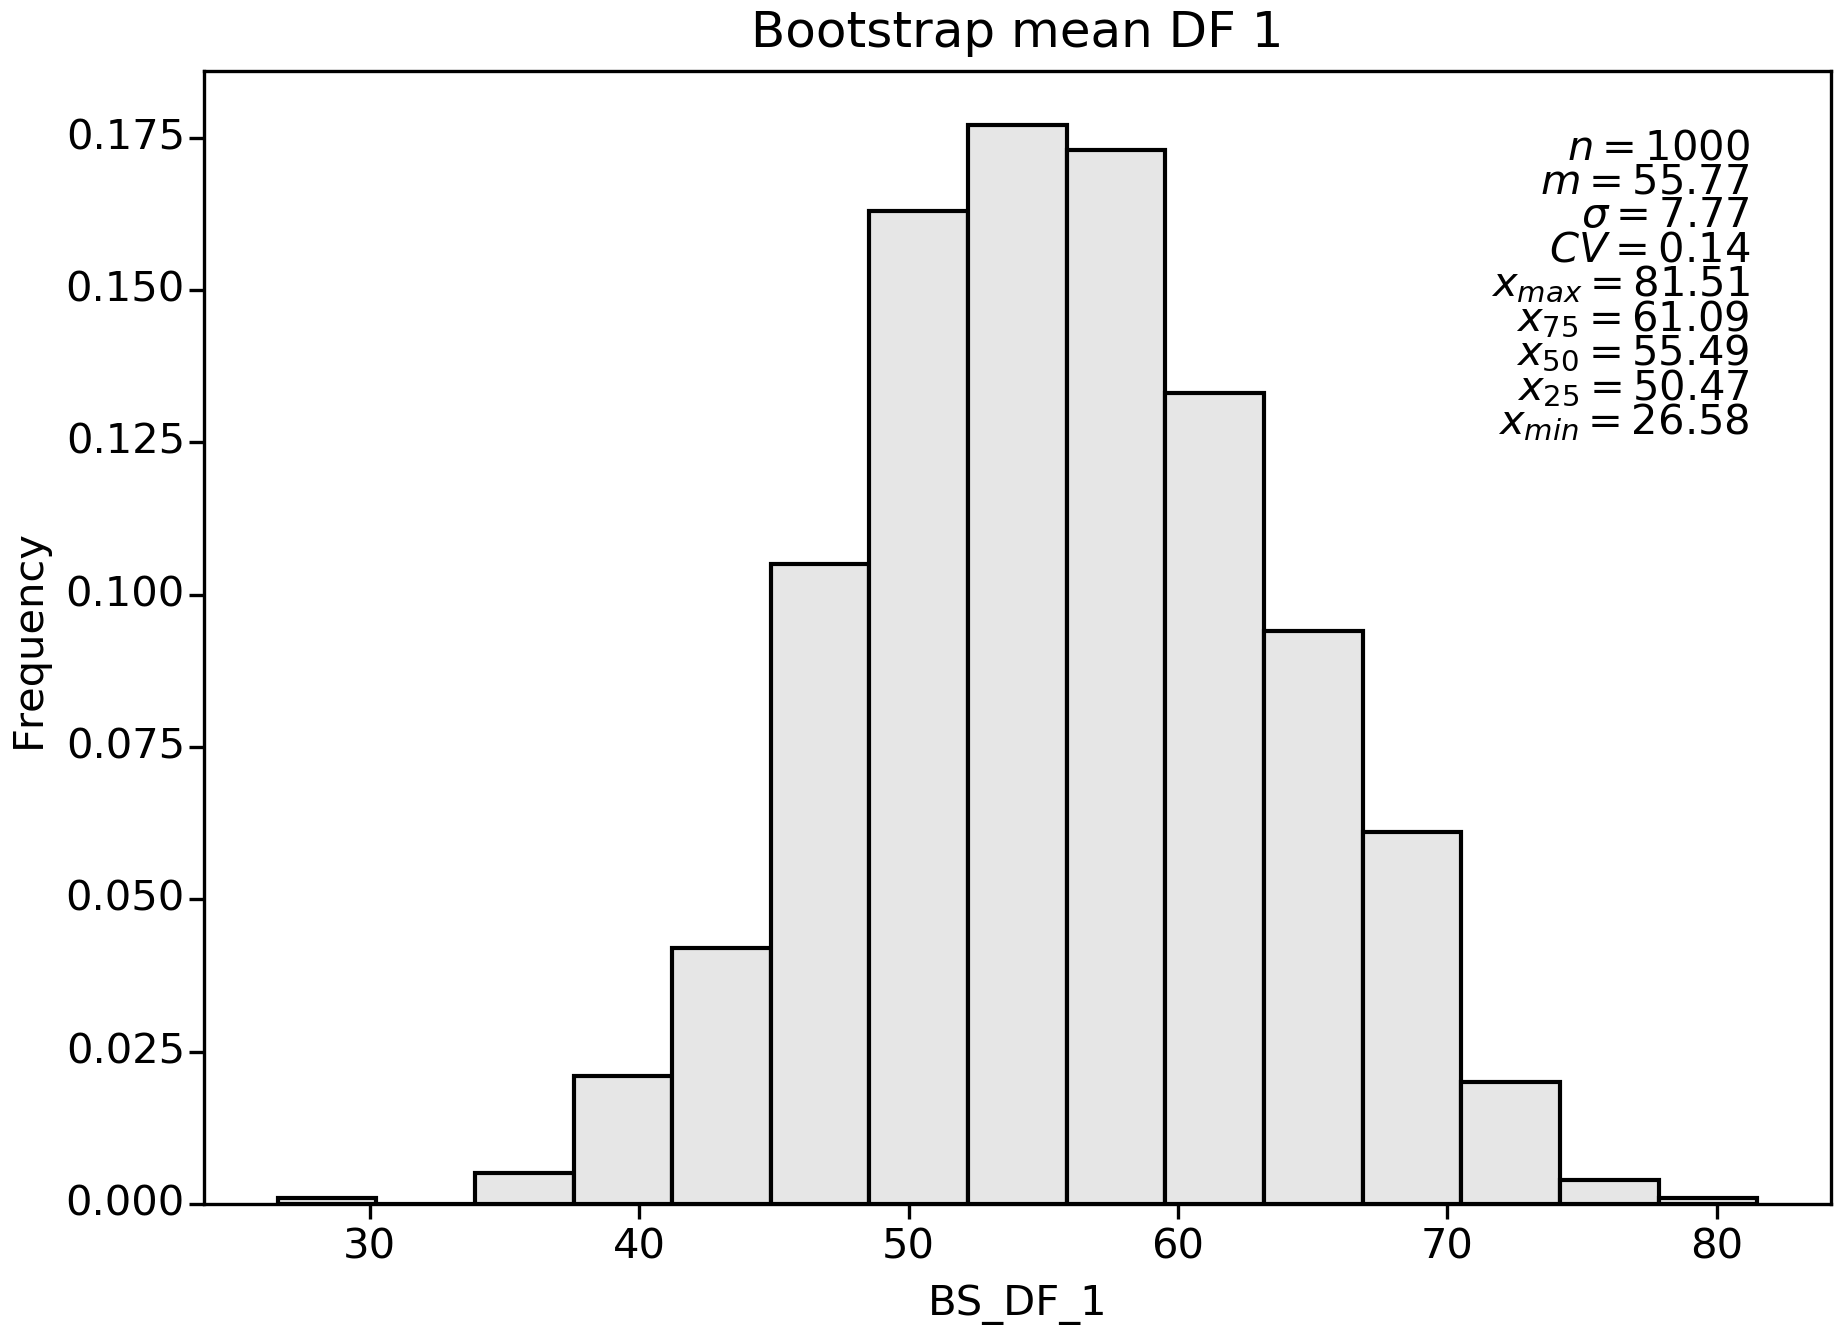
\includegraphics[width=\textwidth]{capitulo_2/BS_DF_1.png}
		\end{center}
		%\legend{Fonte: \citeonline{rolo_dissertacao}}
	\end{figure}
	\end{column}
	\begin{column}{0.5\textwidth}  %%<--- here
	\begin{table}[H]
					\centering
			\begin{tabular}{lr}
				Percentil & \multicolumn{1}{l}{Blocos dentro} \\ \hline
				10 & 109886 \\
				50 & 110446 \\
				90 & 111069 \\ \hline
			\end{tabular}
		\caption{Blocos classificados como pertencentes à categoria 1.}\label{boundsim_table}
	\end{table}
	\end{column}
\end{columns}

\end{frame}

\subsection{Simulação direta das distâncias assinaladas}

\begin{frame}{Simulação direta das distâncias assinaladas}

Simulação direta e classificação dos blocos baseada na menor distância simulada.

O primeiro passo é o cálculo do coeficiente U:

\begin{equation}\label{u_eq}
U(u)=\frac{max\{D_{min}\}-min\{d^*_k(u)\}^K_{k=1}}{max\{D_{min}\}-min\{D_{min}\}}
\end{equation}

Onde:

\begin{equation}
D_{min}=\{min\{d^*_k(u_1)\},...,\{min\{d^*_k(u_n)\}^K_{k=1}\}
\end{equation}

E $d^*_k(u)$ é a distância estimada no local u para a categoria k.


\end{frame}

\begin{frame}{Simulação direta das distâncias assinaladas}
	\begin{figure}[H]
		\caption{\label{u_fig}Coeficiente U calculado para todos os nós do \textit{grid}.}
		\begin{center}
			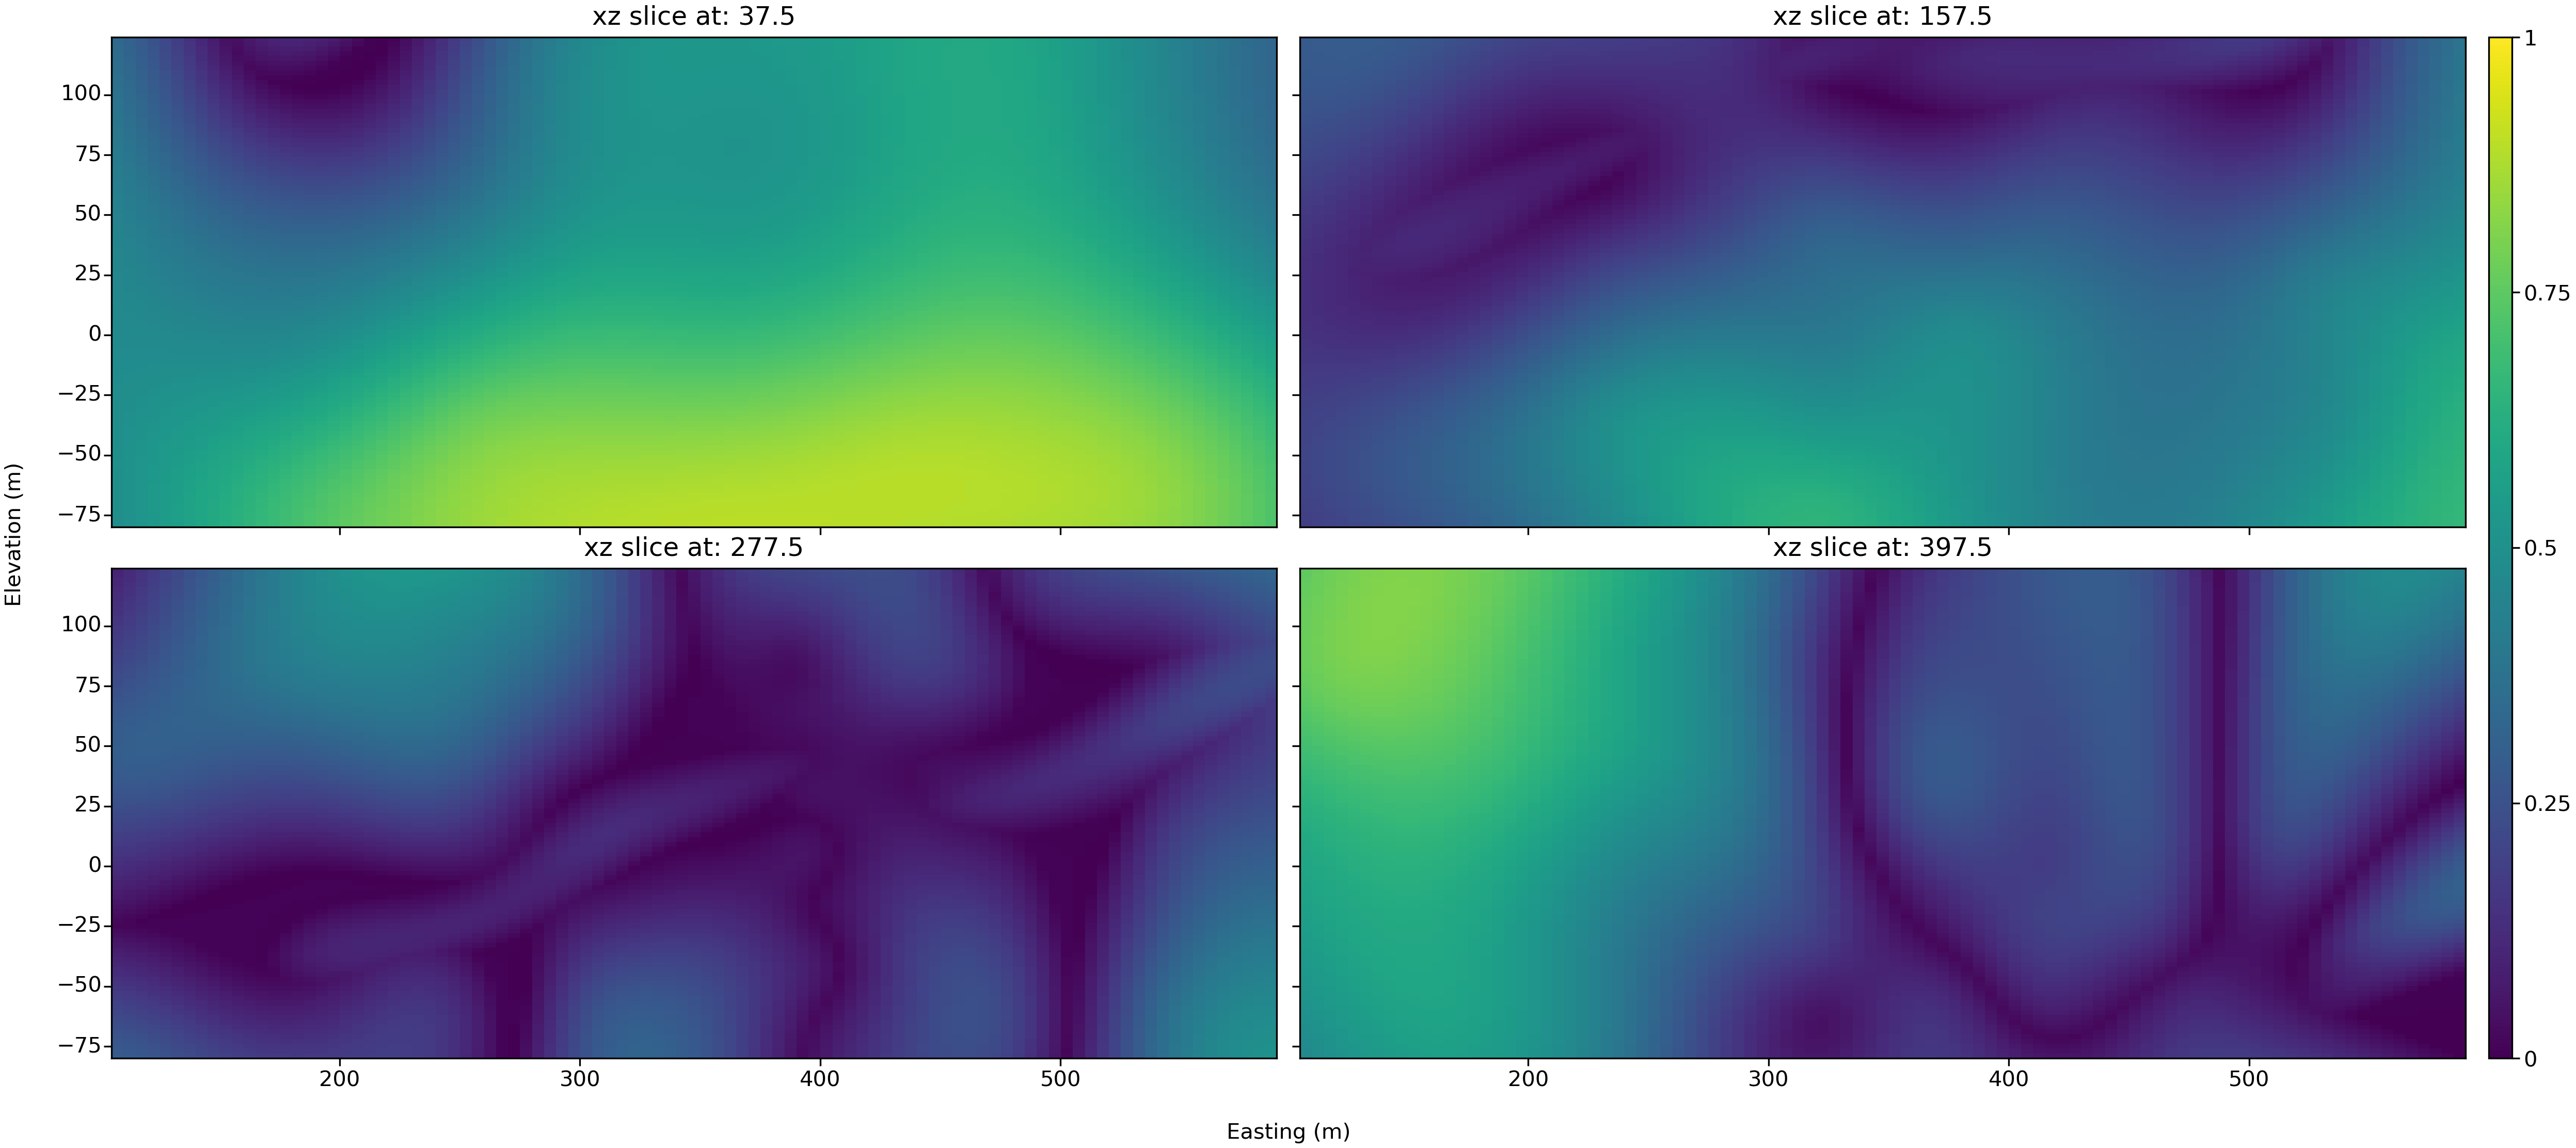
\includegraphics[width=0.8\textwidth]{capitulo_2/u_coef.png}
		\end{center}
		%\legend{Fonte: \citeonline{rolo_dissertacao}}
	\end{figure}
\end{frame}

\begin{frame}{Simulação direta das distâncias assinaladas}

Simulação das distâncias na zona de incerteza:

	\begin{figure}[H] 
		\caption{Distâncias simuladas na zona de incerteza para as categorias do banco de dados.} \label{dist_sim_u}
		\centering
		\subfloat[][Categoria 1]{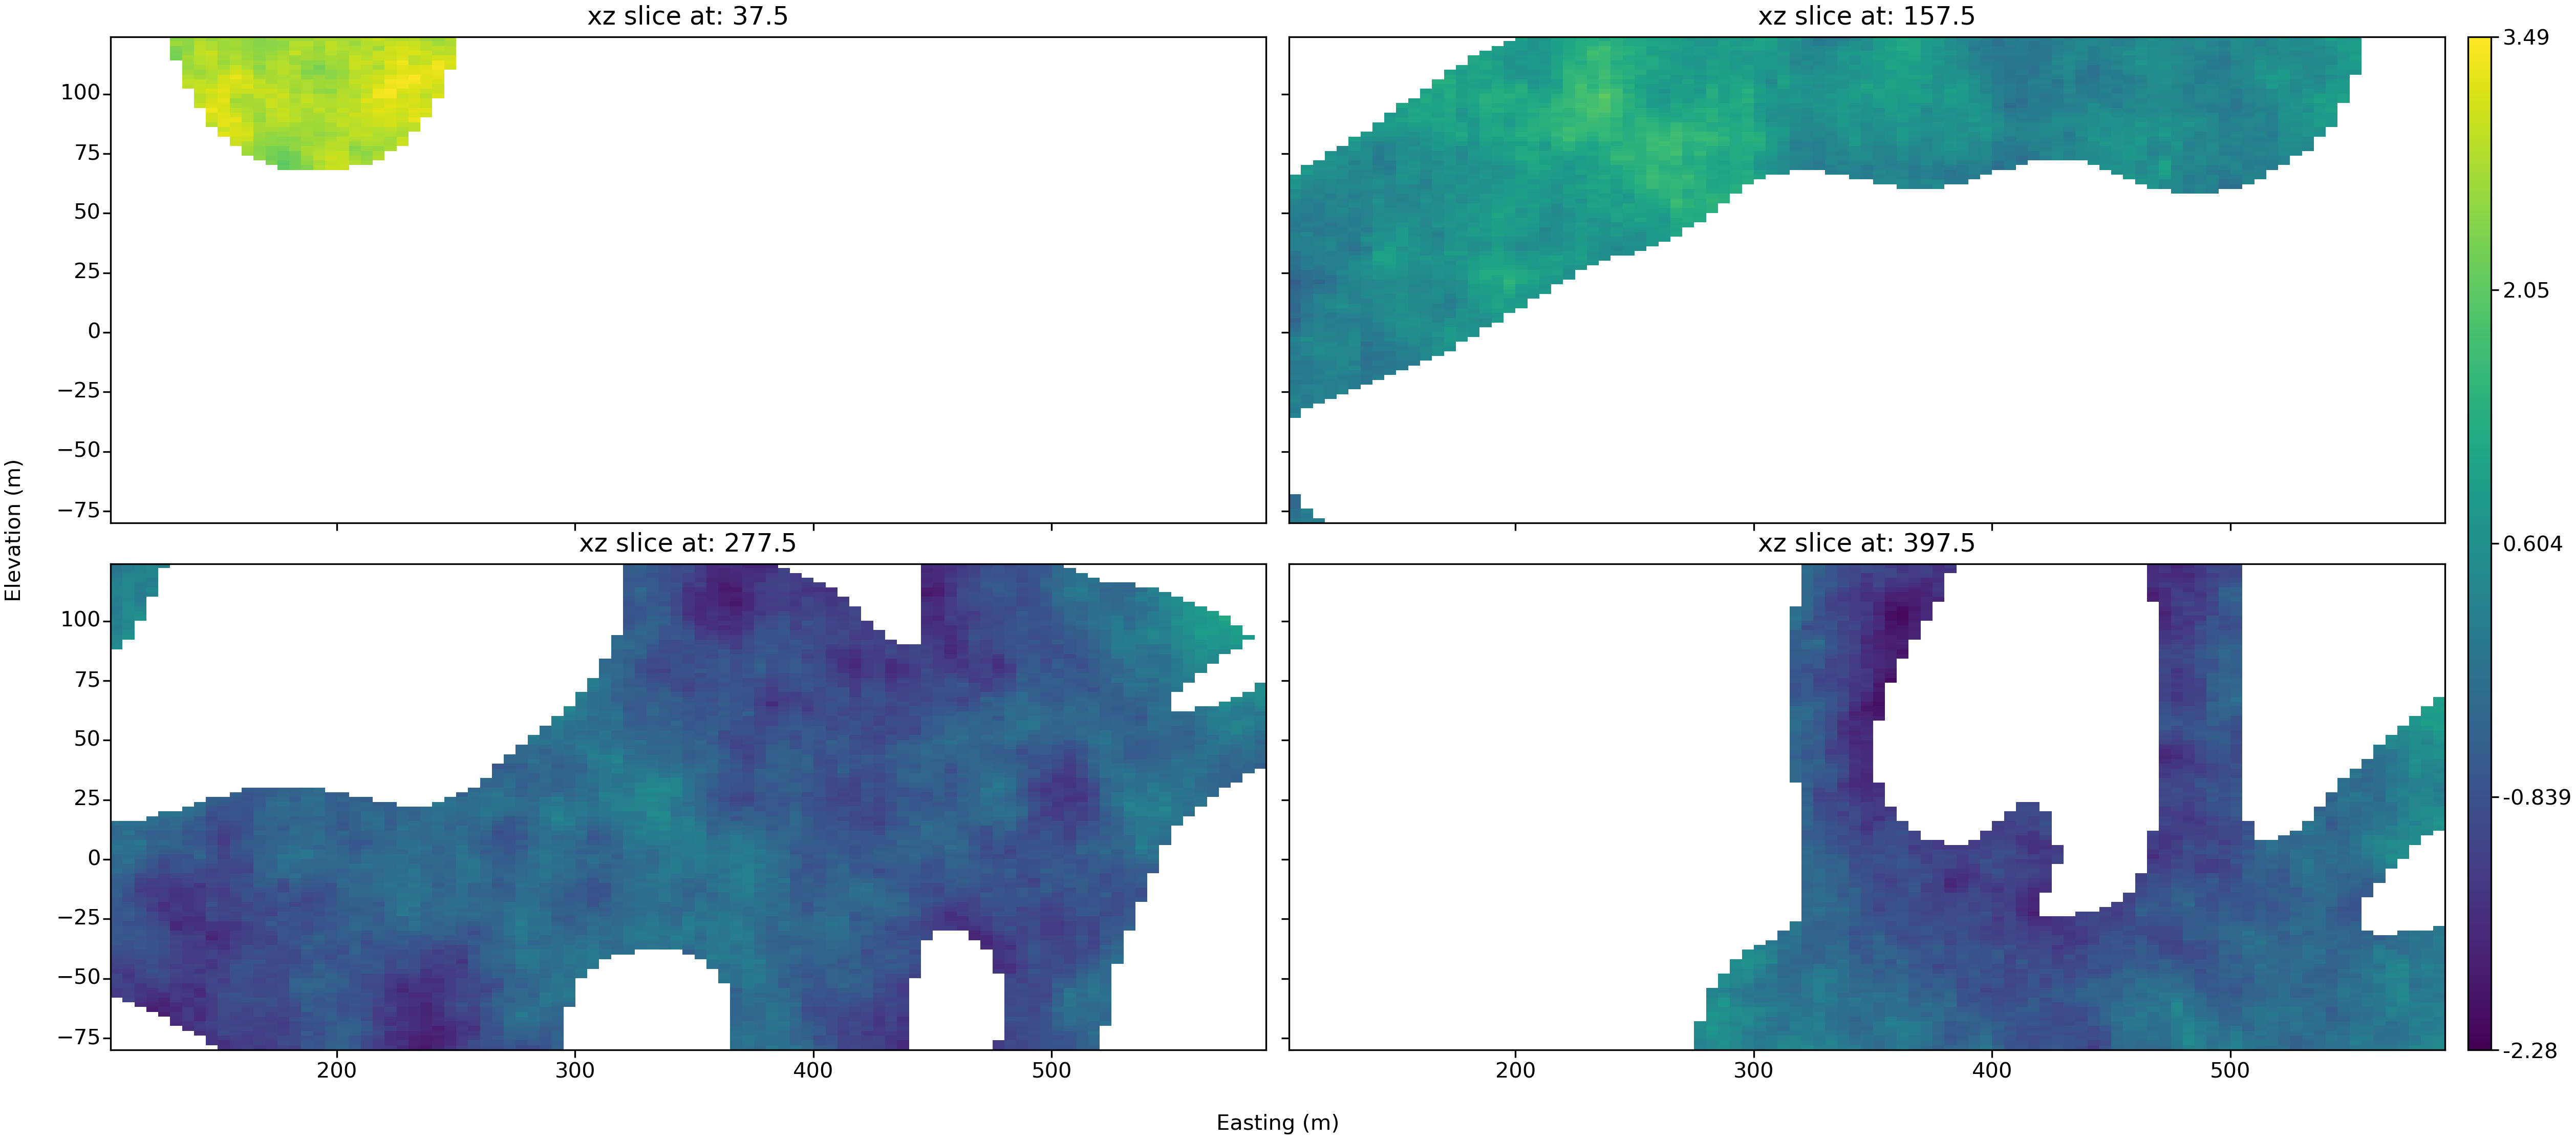
\includegraphics[width=.3\textwidth]{capitulo_2/Ucutoff1.png}\label{<figure1>}}
		\subfloat[][Categoria 2]{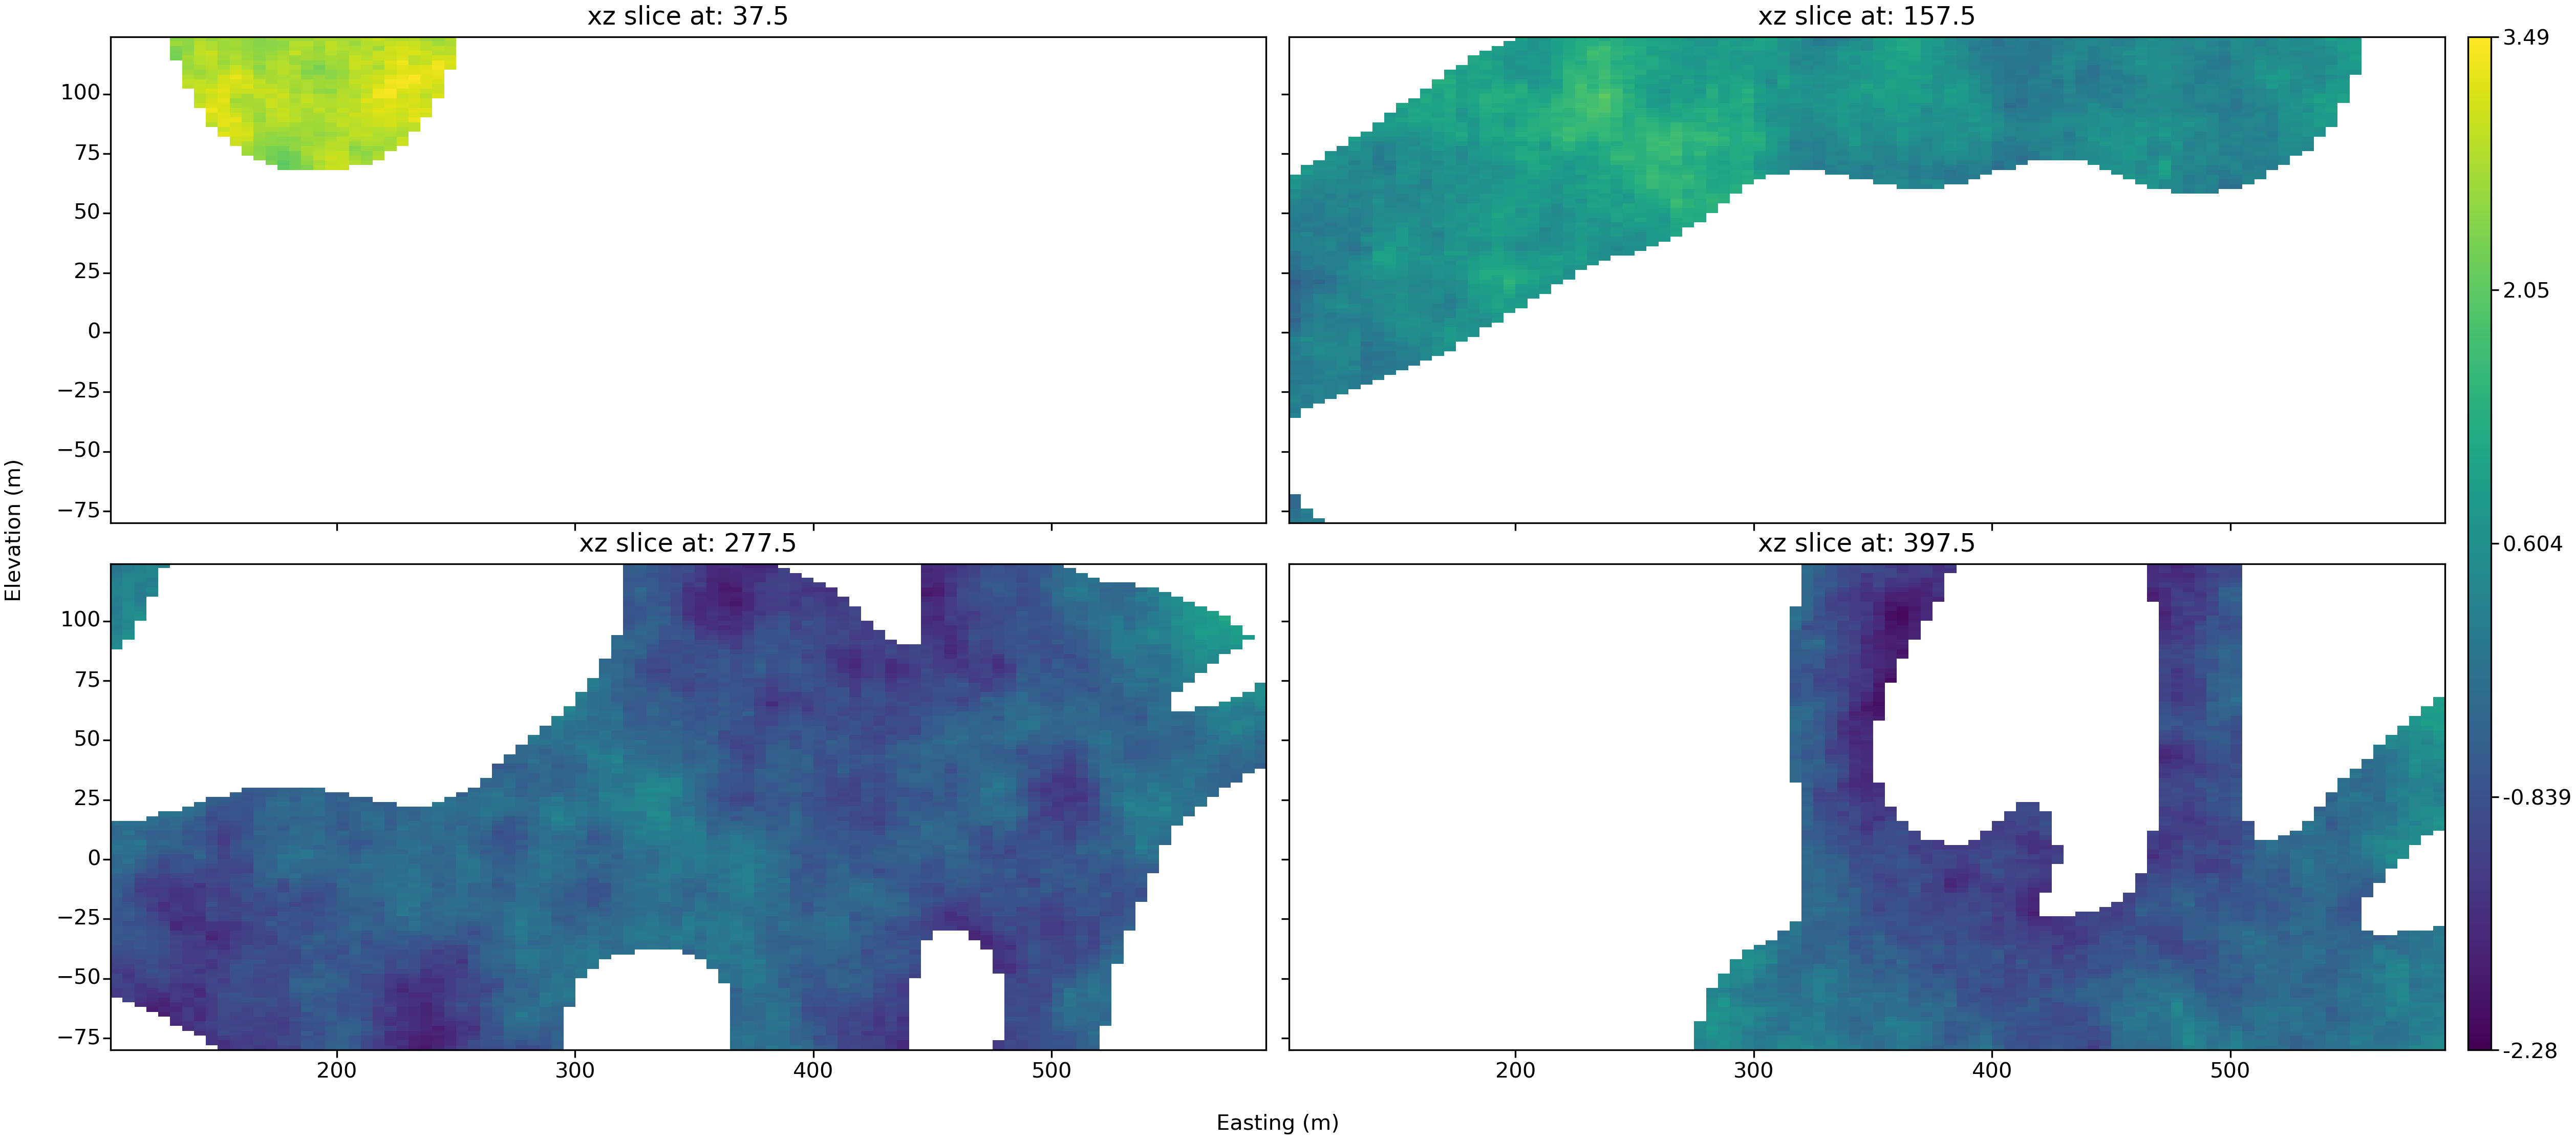
\includegraphics[width=.3\textwidth]{capitulo_2/Ucutoff2.png}\label{<figure2>}}
		\subfloat[][Categoria 3]{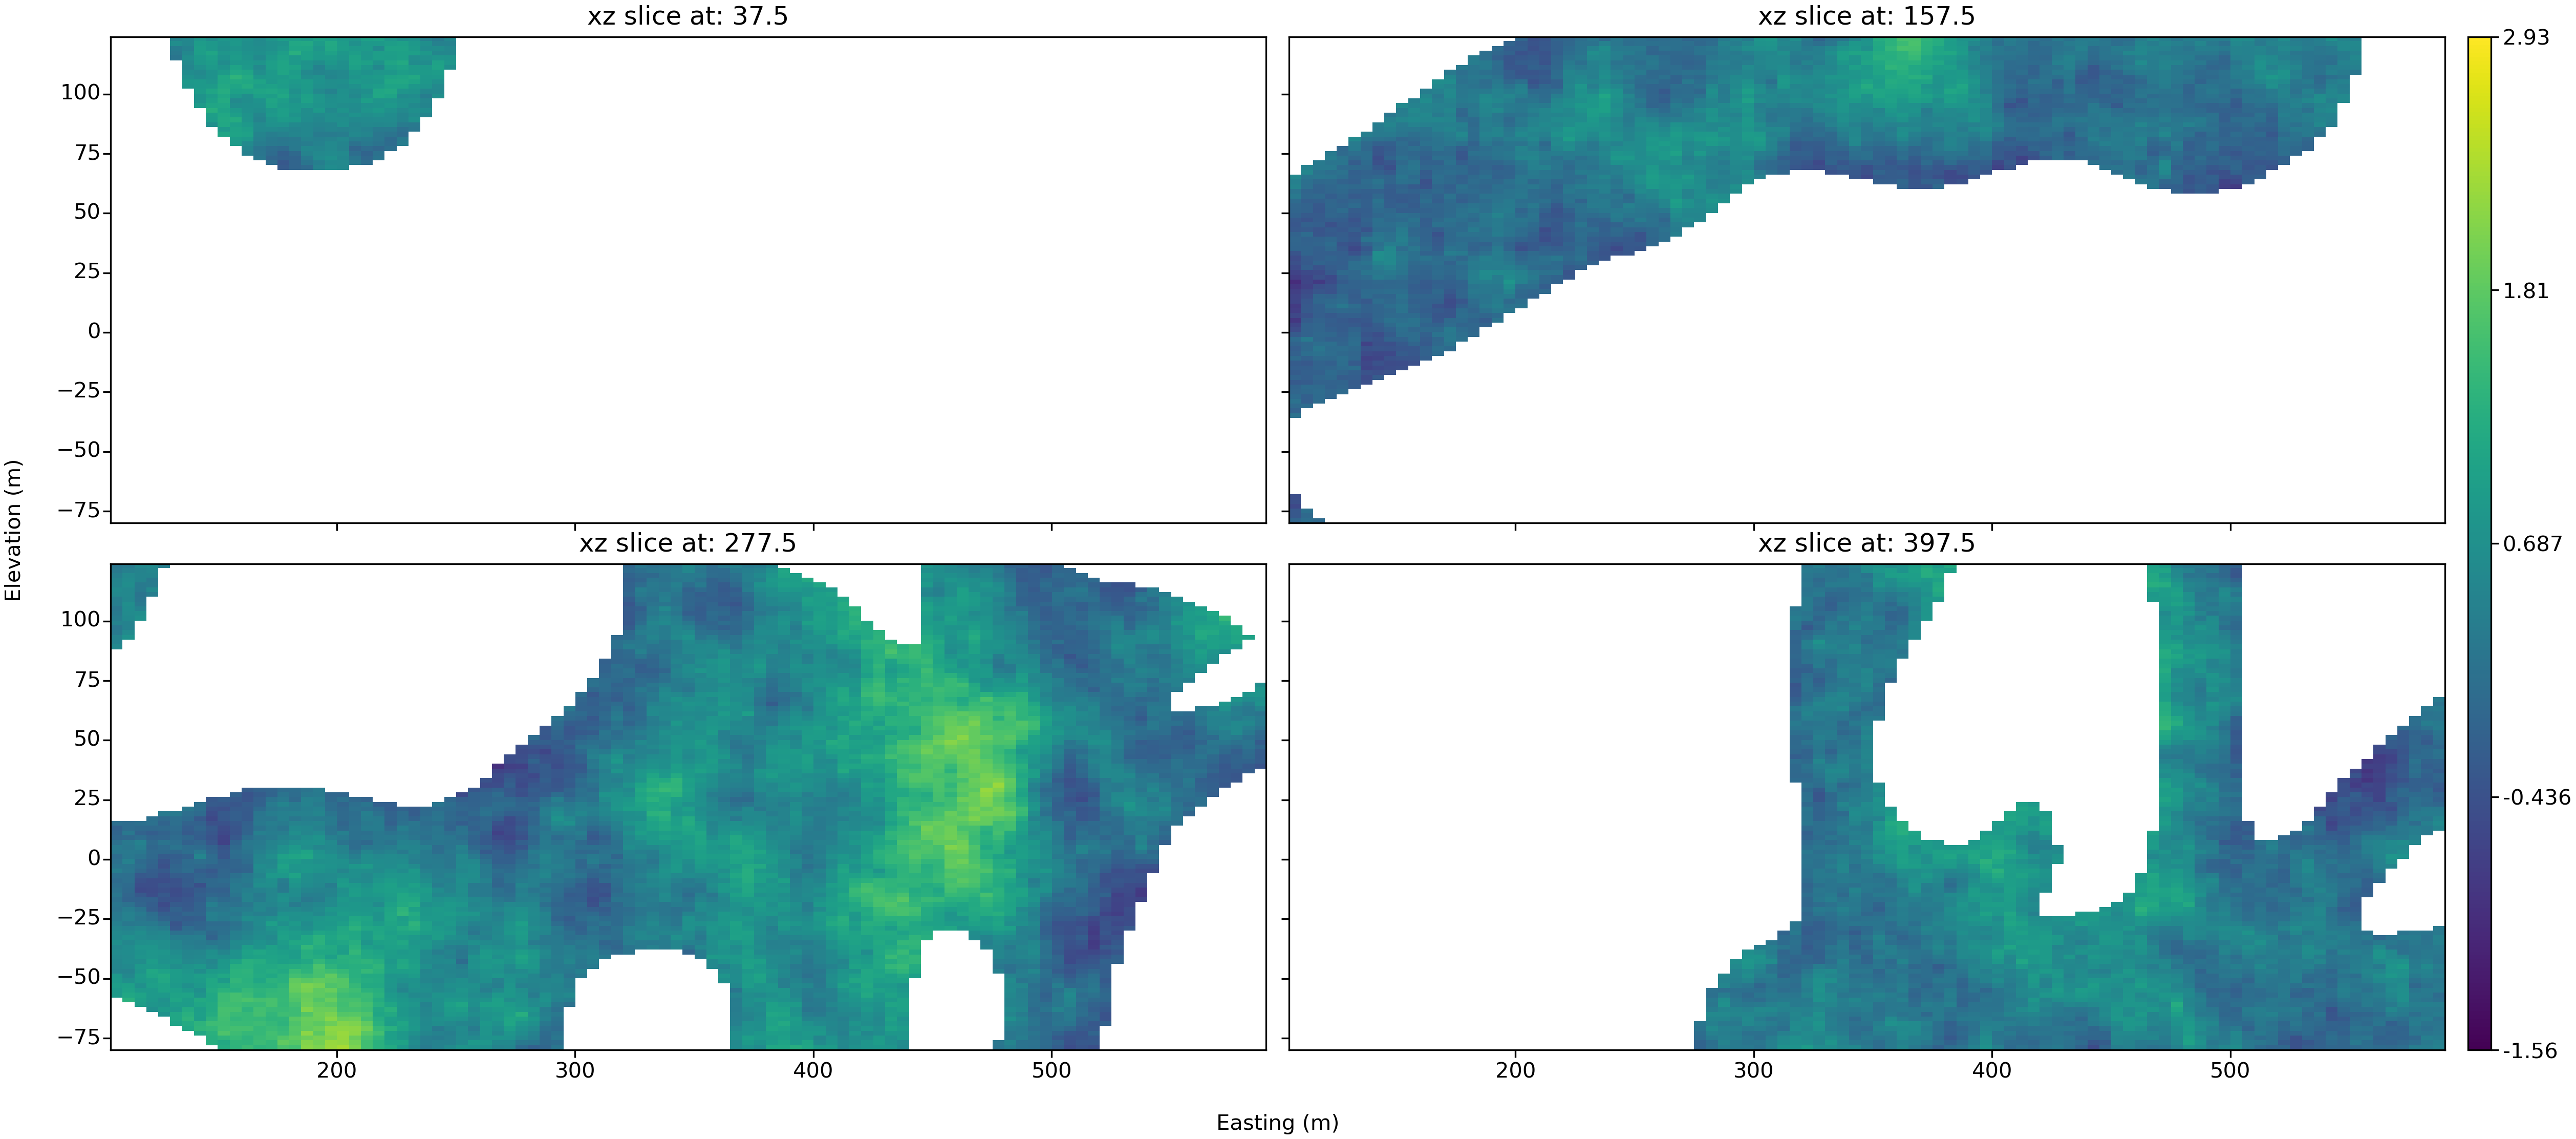
\includegraphics[width=.3\textwidth]{capitulo_2/ucutoff3.png}\label{<figure2>}}
	\end{figure}
\end{frame}

\begin{frame}{Simulação direta das distâncias assinaladas}

Classificação dos blocos.

	\begin{figure}[H]
		\caption{Diferentes realizações do modelo geológico.} 
		\label{dif_real}
			\subfloat[][Realização 1]{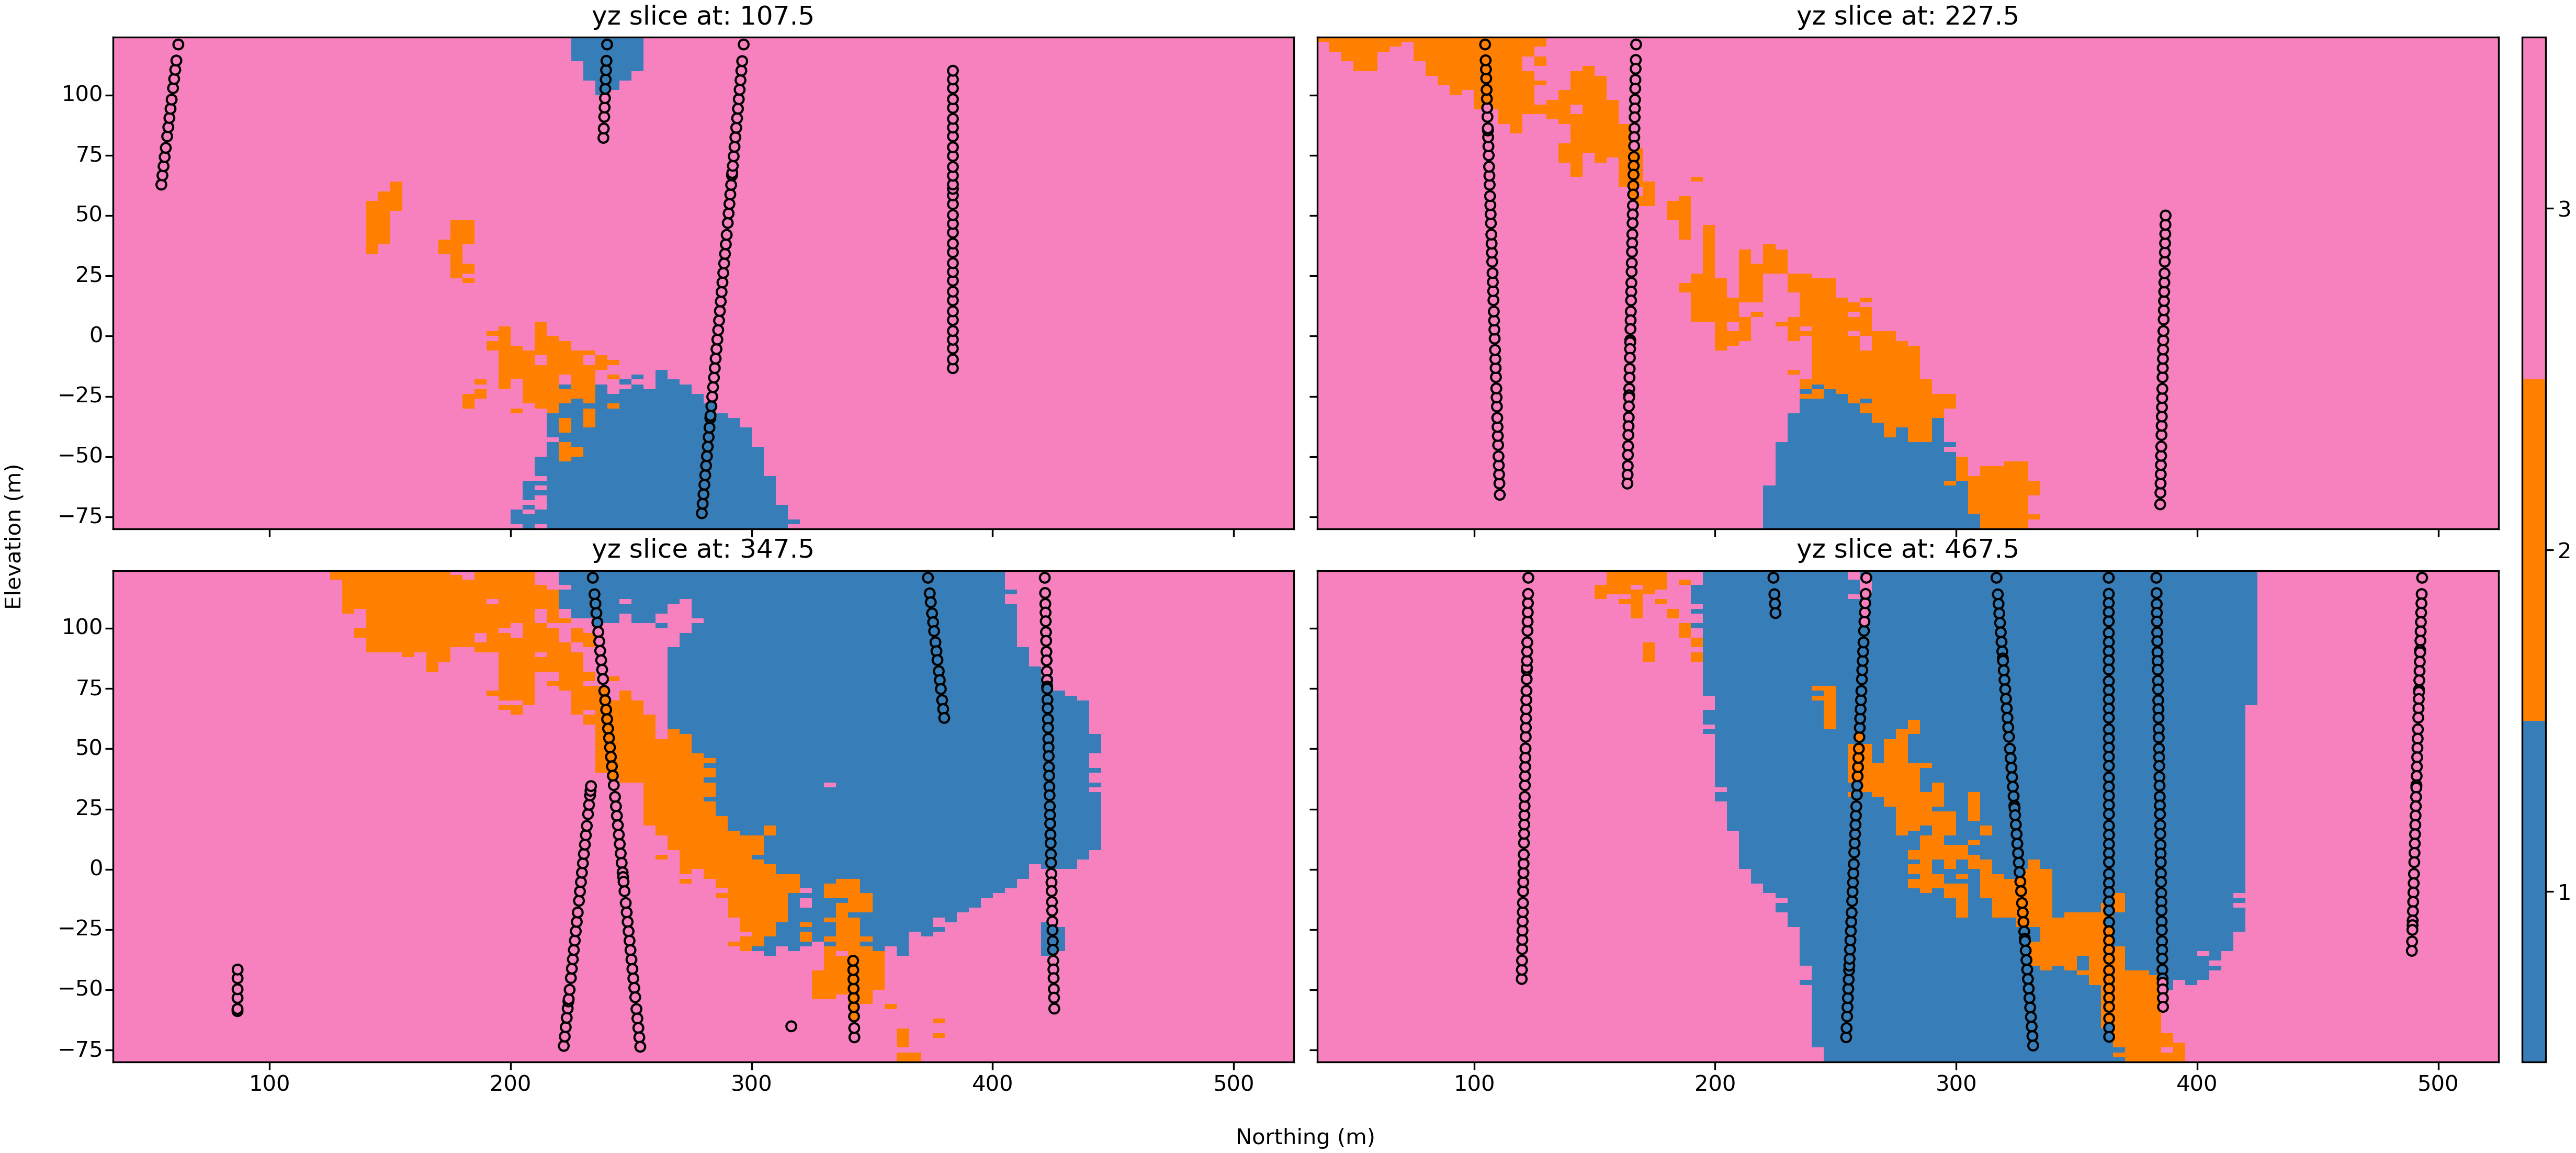
\includegraphics[width=0.5\textwidth]{capitulo_2/directsimreal1.png}\label{a}}
			\subfloat[][Realização 2]{\includegraphics[width=0.5\textwidth]{capitulo_2/directsimreal2.png}\label{b}}
	\end{figure}
\end{frame}

\begin{frame}{Simulação direta das distâncias assinaladas}
	\begin{enumerate}
		\item Cálculo das distâncias assinaladas para todas as amostras e categorias;
		\item Variografia das distâncias no espaço original para todas as categorias;
		\item Interpolação das distâncias; 
		\item criação do modelo com base na menor distância interpolada;
		\item Criação da zona de incerteza;
		\item Transformação Gaussiana das distâncias;
		\item Variografia das distâncias no espaço gaussiano para todas as categorias;
		\item Geração de múltiplos modelos baseados na menor distância simulada;
		\item Validação e pós processamento das realizações.
	\end{enumerate}
\end{frame}

\subsection{Simulação multi ponto}

\begin{frame}{Simulação multi ponto}

MPS em uma TI gerada pela interpolação das distâncias assinaladas.
	\begin{figure}[H]
		\caption{Diferentes realizações do modelo geológico.} 
		\label{snesim_real}
			\subfloat[][Realização 1]{\includegraphics[width=0.5\textwidth]{capitulo_2/snesim_real1.png}\label{a}}
			\subfloat[][Realização 2]{\includegraphics[width=0.5\textwidth]{capitulo_2/snesim_real2.png}\label{b}}
	\end{figure}
\end{frame}

\subsection{Boundary simulation}

\begin{frame}{Boundary simulation}

Comparação de valores simulados e interpolados.

	\begin{equation}
	d_k(u_\alpha)=\begin{cases}
	-\parallel u_\alpha-u_\beta\parallel - C,\:\textrm{se $u_\alpha$ pertence ao domínio}\\
	+\parallel u_\alpha-u_\beta\parallel + C,\:\textrm{se $u_\alpha$ não pertence ao domínio}\end{cases}
	\label{C_dist}
	\end{equation}
	
	\begin{figure}[H]
		\caption{\label{class}Classificação dos locais comparando valores estimados e simulados.}
		\begin{center}
			\includegraphics[width=0.8\textwidth]{capitulo_2/classificacao.png}
		\end{center}
		%\legend{Fonte: Modificado de \citeonline{wilde_sim_bound_reals}}
	\end{figure}
\end{frame}

\begin{frame}{Boundary simulation}

Calibração do parâmetro C:

	\begin{figure}[H]
		\caption{\label{c_param_1}Calibração do parâmetro C para a categoria 1.}
		\begin{center}
			\includegraphics[width=0.6\textwidth]{capitulo_2/uncert_1.png}
		\end{center}
		%\legend{Fonte: \citeonline{rolo_dissertacao}}
	\end{figure}
\end{frame}

\begin{frame}{Boundary simulation}
Para que a simulação seja realizada de forma uniforme entre –C e +C, o desvio padrão $y`(u)$, deve ser simulado e transformado pela relação:


	\begin{equation}
	df'(u)=2*C*G^-1(y'(u))-C
	\end{equation}
	
onde: $df'(u)$ é o valor da função distância simulada, $y'(u)$ o valor normal padrão da simulação não condicional, e $G^-1$ representa a determinação do valor da distribuição acumulada padrão normal correspondente a $y'(u)$. Para garantir que os valores pertençam a região estabelecida, os valores são multiplicados por 2C e subtraídos de C.
	
\end{frame}

\begin{frame}{Boundary simulation}
	\begin{figure}[H] 
		\caption{Interpolação, simulação e classificação na zona de incerteza.} \label{cat1_bound_sim}
		\centering
		\subfloat[][Distâncias interpoladas]{\includegraphics[width=.3\textwidth]{capitulo_2/interpolated.jpeg}\label{<figure1>}}
		\subfloat[][Distâncias simuladas]{\includegraphics[width=.3\textwidth]{capitulo_2/simulated.jpeg}\label{<figure2>}}
		\subfloat[][Classificação]{\includegraphics[width=.3\textwidth]{capitulo_2/classification.jpeg}\label{<figure2>}}
	\end{figure}
\end{frame}

\begin{frame}{Boundary simulation}

Blocos classificados.

	\begin{figure}[H]
		\caption{Seções verticais de uma realização para a categoria 1.} 
		\label{cpar_real}
			\subfloat[][Seção em XY]{\includegraphics[width=0.5\textwidth]{capitulo_2/cpar1.png}\label{a}}
			\subfloat[][Seção em YZ]{\includegraphics[width=0.5\textwidth]{capitulo_2/cparyz.png}\label{b}}
	\end{figure}
\end{frame}

\subsubsection{Abordagem hierárquica}

\begin{frame}{Abordagem hierárquica}
	\begin{figure}[H]
		\caption{\label{hier_ex}Esquema do método mostrando os passos necessários.}
		\begin{center}
			\includegraphics[width=\textwidth]{capitulo_2/hier_example.png}
		\end{center}
		%\legend{Fonte: Modificado de \citeonline{amarante_incerteza_associada}}
	\end{figure}
\end{frame}

\subsection{Sumário dos métodos de avaliação de incerteza}

\begin{frame}{Sumário dos métodos de avaliação de incerteza}
	

	\begin{table}[H]
		\centering
		\resizebox{\textwidth}{!}{
			\begin{tabular}{lcccccc}
				Método & \multicolumn{1}{l}{Simplicidade} & \multicolumn{1}{l}{Velocidade} & \multicolumn{1}{l}{Multi categórico} & \multicolumn{1}{l}{Realismo geológico} & \multicolumn{1}{l}{Controle da incerteza} & \multicolumn{1}{l}{Controle do tipo de contato} \\
				\midrule
				Heurístico & simples & rápido & sim   & não   & sim   & não \\
				Boundsim & simples & rápido & não   & sim   & não   & não \\
				Simulação direta & complexo & demorado & sim   & não   & sim   & não \\
				MPS   & simples & rápido & sim   & sim   & não   & não \\
				Boundary simulation & simples  & rápido & não   & sim   & sim   & sim \\
				\bottomrule
			\end{tabular}
		}
		\caption{Sumário dos métodos de avaliação de incerteza de modelos geológicos.}\label{sumario}%
	\end{table}

\end{frame}

\section{Proposta de tese}

\subsection{Problemas}

\begin{frame}{Problemas}
	\begin{itemize}
		\item Não estacionariedade da função distância assinalada torna a modelagem dos variogramas arbitrária e questionável
		\item não estacionariedade da função distância assinalada torna a modelagem dos variogramas arbitrária e questionável;
		\item É preciso encontrar um balanço entre número de nós e resolução necessária. A resolução do \textit{grid} influencia diretamente a avaliação de incertezas;
		\item A escolha do interpolador muitas vezes é subjetiva e confusa;
		\item Na presença de múltiplos domínios, principalmente em ambientes geológicos complexos, é necessário a aplicação de uma lógica de precedência de estruturas ao invés de simplesmente tomar a menor distância assinalada para a criação de modelos realistas;
		\item Em alguns métodos a definição da zona de incerteza é subjetiva e não segue nenhuma regra matemática ou geológica, em outros a definição da zona de incerteza é extremamente laboriosa e complicada;
		\item Estruturas geológicas específicas, como lentes ou diques, podem desaparecer, ou não serem bem reproduzidas nos modelos implícitos;
		\item É necessário checar se os modelos implícitos honram a geologia do depósito e serão úteis para o processo de avaliação de recursos/reservas.
	\end{itemize}
\end{frame}

\subsection{Interpolador}

\begin{frame}{Interpolador}
	pass
	
\end{frame}

\section{Referências bibliográficas}

\begin{frame}{Referências bibliográficas}
	\bibliographystyle{apa}
	\bibliography{bibliografia}
\end{frame}

\end{document}